%%%%%%%%%%%%%%%%%%%%%%%%%%%%%%%%%%%%%%%%%%%%%%%%%%%%%%%%%%%%
%% WARNING: There should be no reason to edit this file.
%%          This project has been setup so that all files
%%          that need to be edited or added should be done
%%          in one of the directories inside this project.
%%          See the README.md file for an overview of the
%%          project layout.
%%          --DDM
%%%%%%%%%%%%%%%%%%%%%%%%%%%%%%%%%%%%%%%%%%%%%%%%%%%%%%%%%%%%
\documentclass[12pt]{cpthesis}

% MY PACKAGES %
\usepackage{siunitx}
\sisetup{
    detect-all,          % match surrounding font
    per-mode=symbol,     % use "/" for per units
    separate-uncertainty,
    range-phrase=--,
    range-units=single
}
\usepackage{booktabs}

\usepackage{tikz}
\usetikzlibrary{arrows.meta, shapes, positioning, fit}


%%%%%%%%%%%%%%%%%%%%%%%%%%%%%%%%%%%%%%%%%%%%%%%%%%%%%%%%%%%%
%% Math packages
%%%%%%%%%%%%%%%%%%%%%%%%%%%%%%%%%%%%%%%%%%%%%%%%%%%%%%%%%%%%
\usepackage{amsmath}     % for lots math items
\usepackage{amssymb}     % for more math symbols
\usepackage{mathtools}   % for DeclareMathOperator
\usepackage{bm}          % for bold math symbols
\usepackage{bbold}
\usepackage{esvect}
% \DeclareMathAlphabet{\mathbbold}{U}{bbold}{m}{n}
%%%%%%%%%%%%%%%%%%%%%%%%%%%%%%%%%%%%%%%%%%%%%%%%%%%%%%%%%%%%
%% Figures and tables packages
%%%%%%%%%%%%%%%%%%%%%%%%%%%%%%%%%%%%%%%%%%%%%%%%%%%%%%%%%%%%
%% figure related packages
\usepackage{silence}
% This document class is not known to the caption class, but
% there is nothing to be done and the default values are ok.
\WarningFilter{caption}{Unknown document class (or package)}
\usepackage{caption}
\usepackage{subcaption}

\captionsetup{
    format=hang,
    font={it, singlespacing},
    labelfont=bf,
%    textformat=period,
    labelsep=colon
}
\captionsetup[table]{position=above}
\captionsetup[subfigure]{labelformat=parens, font={it, singlespacing}}
\captionsetup[subtable]{labelformat=parens, font={it, singlespacing}, position=top}

% Ensures table floats have caption above table.
% from https://tex.stackexchange.com/a/43097
% Note: Still have to manually do this for non-floating tables.
\usepackage{floatrow}
\floatsetup[table]{capposition=top}

%% table related packages
\usepackage{tabularx}

%% figure related packages
\usepackage{graphicx}

% Add figures folder to the graphics path
\graphicspath{{figures/}}

\newcommand{\printlistoftables}{
    \listoftables
    \addtocontents{lot}{\hbox to \linewidth{\hspace{1.5em}Table\hfill Page}}
}

\newcommand{\printlistoffigures}{
    \listoffigures
    \addtocontents{lof}{\hbox to \linewidth{\hspace{1.5em}Figure\hfill Page}}
}

%%%%%%%%%%%%%%%%%%%%%%%%%%%%%%%%%%%%%%%%%%%%%%%%%%%%%%%%%%%%
%% Nomenclature packages
%%%%%%%%%%%%%%%%%%%%%%%%%%%%%%%%%%%%%%%%%%%%%%%%%%%%%%%%%%%%
\usepackage[intoc,notocbasic]{nomencl}
% changes to formatting of the list of symbols to be upper case
\renewcommand{\nomname}{\MakeUppercase{\listsymbolsname}}
% allow cross-references to the nomenclature
% see: https://tex.stackexchange.com/a/158934
\usepackage{etoolbox}
\patchcmd{\thenomenclature}
  {\chapter*{\nomname}}
  {\phantomsection\chapter*{\nomname}\label{sec:Nomenclature}}
  {}
  {}
\makenomenclature

%%%%%%%%%%%%%%%%%%%%%%%%%%%%%%%%%%%%%%%%%%%%%%%%%%%%%%%%%%%%
%% Bibliography packages
%%%%%%%%%%%%%%%%%%%%%%%%%%%%%%%%%%%%%%%%%%%%%%%%%%%%%%%%%%%%
\usepackage[
    backend=biber,
    style=numeric,
    url=true,
    giveninits=true,
    maxnames=4,
    minnames=3,
]{biblatex} % bibliography
%\AtEveryBibitem{\clearlist{language}}
%\AtEveryBibitem{\clearfield{note}}
\addbibresource{bibliography/references.bib}

%%%%%%%%%%%%%%%%%%%%%%%%%%%%%%%%%%%%%%%%%%%%%%%%%%%%%%%%%%%%
%% Algorithm and code listing packages
%%%%%%%%%%%%%%%%%%%%%%%%%%%%%%%%%%%%%%%%%%%%%%%%%%%%%%%%%%%%
\usepackage{xpatch}
\usepackage[chapter]{algorithm}
\usepackage[noEnd=true, indLines=true]{algpseudocodex}
\captionsetup[algorithm]{labelsep=colon}
% remove top rule for algorithm environment
% https://tex.stackexchange.com/a/180337
\DeclareFloatStyle{rulednotop}{midcode=rule,postcode=lowrule,capposition=top,heightadjust=all}
\floatsetup[algorithm]{style=rulednotop}
\renewcommand{\listalgorithmname}{\MakeUppercase{\listalgorithmsname}}
\addtocontents{loa}{\hbox to \linewidth{\hspace{1.5em}Algorithm\hfill Page}}

%%%%%%%%%%%%%%%%%%%%%%%%%%%%%%%%%%%%%%%%%%%%%%%%%%%%%%%%%%%%
%% Code and code listing packages
%%%%%%%%%%%%%%%%%%%%%%%%%%%%%%%%%%%%%%%%%%%%%%%%%%%%%%%%%%%%
\usepackage{listings}
\lstset{
    basicstyle=\linespread{1.0}\ttfamily,
%    numbers=left,
    breaklines=true,
    xleftmargin=5ex,
    frame=lines,
}
\renewcommand{\lstlistlistingname}{\MakeUppercase{\listcodelistingsname}}
\renewcommand{\lstlistingname}{Code Listing}
\addtocontents{lol}{\hbox to \linewidth{\hspace{1.5em}Code Listing\hfill Page}}

%%%%%%%%%%%%%%%%%%%%%%%%%%%%%%%%%%%%%%%%%%%%%%%%%%%%%%%%%%%%
%% Additional packages needed for specific thesis
%%%%%%%%%%%%%%%%%%%%%%%%%%%%%%%%%%%%%%%%%%%%%%%%%%%%%%%%%%%%
%%%%%%%%%%%%%%%%%%%%%%%%%%%%%%%%%%%%%%%%%%%%%%%%%%%%%%%%%%%%
%% These packages/settings should be the ones that are
%% specifically needed for your thesis.
%%%%%%%%%%%%%%%%%%%%%%%%%%%%%%%%%%%%%%%%%%%%%%%%%%%%%%%%%%%%

%% This is to create placeholder text and shouldn't be in your thesis
\usepackage{lipsum}

%% TikZ packages
\usepackage{tikz}      % Base package needed for drawing TikZ figures
\usetikzlibrary{calc}  % Needed to do coordinate calculations such as ($(a)!0.5!(b)$)

%% This code creates groups in the nomenclature
% based on Overleaf documentation
% https://www.overleaf.com/learn/latex/Nomenclatures
\usepackage{etoolbox}
\renewcommand\nomgroup[1]{%
    \item[\bfseries
        \ifstrequal{#1}{P}{Physics constants}{%
        \ifstrequal{#1}{N}{Number sets}{%
        \ifstrequal{#1}{O}{Other symbols}{}}}%
    ]
}


%%%%%%%%%%%%%%%%%%%%%%%%%%%%%%%%%%%%%%%%%%%%%%%%%%%%%%%%%%%%
%% hyperlinks and URL handling
%% Note: must be one of the last packages added
%%%%%%%%%%%%%%%%%%%%%%%%%%%%%%%%%%%%%%%%%%%%%%%%%%%%%%%%%%%%
\usepackage{url}
\usepackage[breaklinks=true,hidelinks,pdfusetitle]{hyperref}
% Options for hyperref
\hypersetup{
    bookmarksnumbered=true,
    bookmarksopen=false,
    bookmarksopenlevel=0,
    colorlinks=false,
    pdfstartview=Fit,
    pdfborder={0 0 0},
}
% remove \uppercase from references to chapters
% see: https://tex.stackexchange.com/a/417078
\pdfstringdefDisableCommands{\let\uppercase\@firstofone}
% Make URLs use same typeface as rest of document
\urlstyle{same}

%%%%%%%%%%%%%%%%%%%%%%%%%%%%%%%%%%%%%%%%%%%%%%%%%%%%%%%%%%%%
%% Automatic determination of kind of reference
%% Note: must be included after hyperref
%%%%%%%%%%%%%%%%%%%%%%%%%%%%%%%%%%%%%%%%%%%%%%%%%%%%%%%%%%%%
\RequirePackage{cleveref}
% Define Appendix refs
\crefname{app}{appendix}{appendices}
\Crefname{app}{Appendix}{Appendices}
% oxford comma
\newcommand{\creflastconjunction}{, and~}

%%%%%%%%%%%%%%%%%%%%%%%%%%%%%%%%%%%%%%%%%%%%%%%%%%%%%%%%%%%%
%% End of document preamble
%%%%%%%%%%%%%%%%%%%%%%%%%%%%%%%%%%%%%%%%%%%%%%%%%%%%%%%%%%%%

% Setting for the front matter
\title{Title of Thesis in All Caps, Inverted Pyramid Style if More Than One Line and if More Than Two Lines Then Spacing Needs to be Consistent}
\author{Your Name}
\degreemonth{June}
\degreeyear{2024}
\degree{Master of Science}
\field{Your Degree}
\numberofmembers{4}
   \chair{Misty Mustang, Ph.D. \linebreak Professor of Animal Science}
   \othermemberA{Faculty Member, Ph.D. \linebreak Professor of Some Department}
   \othermemberB{Another Faculty, Ph.D. \linebreak Professor of Some Department}
   \othermemberC{Outside Advisor \linebreak CTO, External Organization Name}
   \othermemberD{Awesome Lecturer, M.S. \linebreak Lecturer of Some Department}
   \othermemberE{Faculty Member, VI, Ph.D. \linebreak Professor of Some Department}
   \othermemberF{Faculty Member, VII, Ph.D. \linebreak Professor of Some Department}
   \othermemberG{Faculty Member, VIII, Ph.D. \linebreak Professor of Some Department}
   \othermemberH{Faculty Member, IX, Ph.D. \linebreak Professor of Some Department}
   \othermemberI{Faculty Member, X, Ph.D. \linebreak Professor of Some Department}
\keywords{Select descriptive keywords and separate terms with a comma and a space.}


\begin{document}
    %% The content before first chapter
    \begin{frontmatter}
        \maketitle

        % Custom made for Cal Poly (by Mark Barry, modified by Andrew Tsui).
        \copyrightpage

        % Custom made for Cal Poly (by Andrew Tsui).
        \committeemembershippage

        % Abstract page
        \begin{abstract}
            This thesis greatly advances the capabilities of Cal Poly's 
Spacecraft Attitude Dynamic's Simulator through the design,
integration, and test of a new automatic mass balancing system.
Balancing results are  an improvement over previous iterations 
of the simulator, and align with the results of other universities
in recent years.
        \end{abstract}

        % Acknowledgments page (if wanted)
        % if only have one acknowledgment then uncomment this line
%\renewcommand{\acknowledgename}{Acknowledgment}

\begin{acknowledgments}

 

    Thanks to:
    \begin{itemize}
        \item Andrew Guenther, for uploading the original template, and
        \item Someone Else, so that I do not have to rename this page.
    \end{itemize}
\end{acknowledgments}


        % Dedication page (if wanted)
        \begin{dedication}
    This is optional, but can be included if desired.
    If no dedication, delete the contents of the dedication file.
\end{dedication}


        % Insert table of contents
        \tableofcontents

        % Insert all of the potentially optional listings
        %% For any listing that is empty, then comment out/remove that code.

% Insert list of tables
\printlistoftables

% Insert list of figures
\printlistoffigures

% Insert list of symbols
\printnomenclature


        % Insert list of symbols
        % Note: package handles inserting into table of contents

    \end{frontmatter}

    %% Input the chapters as configured from the file
    \chapter{Introduction}

\section{Motivation}
Spacecraft dynamics simulators are used extensively in the development and testing of all modern space systems [1]. The ability of space organizations to test both their flight hardware and software before launch is a crucial part in reducing on-orbit
failures. The primary goal of all spacecraft dynamics simulators is to recreate the frictionless, torque-free environment of space. The approaches to this goal vary slightly as will be discussed in Chapter 2, but the primary method mounts the spacecraft hardware to a spherical air-bearing, allowing the platform to freely rotate about its yaw axis, and within some limited range about it's pitch and roll axes. The high pressure air between the spherical mount and platform ensures rotation with near-zero friction [2].

While an air-bearing helps guarantee frictionless rotation, any distance between the platform's center of mass and it's center of rotation will introduce a torque due to gravity that is not seen in space. Simulator's are able to shift their center of mass by changing the position of sliding masses onboard \cite{kim_automatic_2009}. The end goal is to adjust the mass blocks' positions such that the mass distribution of the platform changes, and the distance between the platform's center of mass and center of rotation is minized. These masses may be adjusted by hand with visual inspection (referred to as manual mass balancing), or they may be precisely controlled using a preset balancing algorithm and linear actuators (referred to as automatic mass balancing). The detailed requirements of a mass balancing system will be discussed in \Cref{chap:background}, but in general, all simulators must perform some form of balancing this balancing process should both minimize the torque due to gravity and run as fast as possible.



\section{Previous Work}

Research laboratories and universities take part in building their own simulators for educational purposes and as a way to test novel control algorithms and hardware. The Cal Poly Spacecraft Attitude Dynamics Simulator (SADS) is part of this category and has been developed by students and faculty over the years \cite{mittelsteadt_cal_2007}. The mass balancing system on the SADS has gone under numerous iterations which are summarized in Table



\section{Thesis Objectives}


- Create a balancing system that can be run quickly and achieves similar or better balancing results than previous iterations

- Advance work on the SADS overall design that will be necessary for other subsystems, namely a measurement system and early iteration of a flight computer, track lessons learn

- Compare the results of various balancing methods found in literature on the same platform, provide a clear comparison to theortical and real results, provide practical insights on MBS design and implementation (there is an apprent gap for this in literature, with an abundance of papers providing theoretical approaches, but few providing experimental results, and fewer discussing the details of said experiments)


\chapter{Background}

\section{Mass Balancing Systems}

\section{Batch Estimation Algorithms}

\section{Kalman Filtering for Inbalance Estimation}

\section{Active Control for Balancing}

\chapter{Methodology}\label{chap:methodology}

\section{Theoretical Framework}
\subsection{Problem Definition}\label{sec:mbs_problem}

\begin{figure}
    \centering
    \usetikzlibrary{arrows.meta,3d}
\begin{tikzpicture}[scale=3, line cap=round, line join=round]

% Inertial frame (I)
\draw[->, thick] (0,0) -- (2,0) node[below right] {$\hat{x}_N$};
\draw[->, thick] (0,0) -- (0,2) node[above left] {$\hat{y}_N$};
\draw[->, thick] (0,0) -- (-1.2,-1.2) node[below right] {$\hat{z}_N$};
\node[below right] at (0,0) {$O$};

% Cylinder representing platform ------------------------------
\pgfmathsetmacro{\radius}{1.1}
\pgfmathsetmacro{\height}{0.9}

\begin{scope}[rotate around={20:(0,0)}] 
    \draw[gray,dashed] (0,-\height/2) ellipse ({\radius} and 0.2);
    \draw[gray,dashed] (0,\height/2) ellipse ({\radius} and 0.2);
    \draw[gray,dashed] (-\radius,-\height/2) -- (-\radius,\height/2);
    \draw[gray,dashed] (\radius,-\height/2) -- (\radius,\height/2);
\end{scope} 

% Body frame (B), shifted and rotated
\begin{scope}[rotate=20]
    \draw[->, thick, red] (0,0) -- (1.2,0) node[below right] {$\hat{x}_B$};
    \draw[->, thick, red] (0,0) -- (0,1.2) node[above left] {$\hat{y}_B$};
    \draw[->, thick, red] (0,0) -- (-0.7,-0.7) node[below right] {$\hat{z}_B$};
    % \node[below left, red] at (0,0) {$\mathcal{B}$};

    % START M2 --------------------------------------
    \draw[->] (0,0) -- (-0.2,0.5) coordinate (rho2_end) 
        node[pos=0.65, below] {$\rho_2$};

    \draw[->, dashed] (rho2_end) -- ++(0,0.5) coordinate (u2_end)  
        node[above left] {$u_2$};

    \path (rho2_end) -- (u2_end) 
        node[pos=0.7, circle, fill=black, inner sep=1.5pt, label=left:$m_2$] {};

    % START M1 --------------------------------------
     \draw[->] (0,0) -- (0.8,0.2) coordinate (rho1_end) 
        node[midway, above] {$\rho_1$};

    \draw[->, dashed] (rho1_end) -- ++(0.5,0) coordinate (u1_end)  
        node[above left] {$u_1$};

    \path (rho1_end) -- (u1_end) 
        node[pos=0.3, circle, fill=black, inner sep=1.5pt, label=below right:$m_1$] {};

    % START M3 -----------------------------------
    \draw[->] (0,0) -- (-0.6,0.1) coordinate (rho3_end) 
        node[midway, below] {$\rho_3$};

    \draw[->, dashed] (rho3_end) -- ++(-0.3,-0.3) coordinate (u3_end)  
        node[below left] {$u_3$};

    \path (rho3_end) -- (u3_end) 
        node[pos=0.3, circle, fill=black, inner sep=1.5pt, label=left:$m_3$] {};
\end{scope}

% START COM r ----------------------------------
\draw[->, thick] (0,0) -- (0.2, -0.65) coordinate (r_end)
    node[below, right] {$\mathbf{r}$};
 




\end{tikzpicture}
    \caption{The mass balancing problem for air bearing based spacecraft dynamics simulators}
    \label{fig:mbs_problem}
\end{figure}


\Cref{fig:mbs_problem} defines the geometery of the problem in a general case. $O$ represents the common origin of the inertial frame $\mathcal{N}$ and the body-fixed principle frame of the simulator $\mathcal{B}$. $O$ is chosen to be the center of rotation. If frictionless rotation is assumed, then the simulator follows Euler's rotational equations of motion with gravity acting as a torque. 

\begin{equation}
    \bm{J}\,\dot{\bm{\omega}} + \bm{\omega}^{\times}\,\bm{J}\bm{\omega} = \bm{T}_g
\end{equation}

Here, $\bm{J}$ is the inertia of the simulator about $O$, $\bm{\omega}$ is the angular velocity of the simulator, and $\bm{T}_g$ is the torque due to gravity. $\dot{\bm{v}}$ represents the time derivative of some vector $\bm{v}$, and $\bm{v}^{\times}$ represents the skew-symmetric cross-product matrix of $\bm{v}$. All vectors and inertias are expressed in $\mathcal{B}$. In general it is more convienent to expand $\bm{T}_g$ which leads to

\begin{equation}\label{equation:starting_eom}
    \bm{J}\,\dot{\bm{\omega}} + \bm{\omega}^{\times}\,\bm{J}\bm{\omega} = m_s\bm{r}^{\times}\bm{g}
\end{equation}

where $m_s$ is the total mass of the simulator, $\bm{r}$ is the center of mass relative to $O$, and the $\bm{g}$ is the accleration due to gravity.

\Cref{fig:mbs_problem} also shows the introduction of three sliding masses, although in general there may be as many as $n$ sliding masses. Each mass $m_i$ has one translational degree of freedom along $\bm{u}_i$, and $\bm{\rho}_i$ represents the position of the $i$-th mass in it's homed position. Since in practice each mass can only travel some limited distance along $\bm{u}_i$, the homed position of a mass is typically chosen as the center of this range of positions. The position relative to $O$ of any mass $\bm{R}_i$ can be obtained with 
\begin{equation}\label{equation:sliding masses}
    \bm{R}_i = \bm{\rho}_i + d_i\bm{u_i}
\end{equation}
where $d_i$ is the distance a mass $m_i$ has travelled along $u_i$ relative to it's zeroed position. More generally, $\Delta\,d_i$ is defined as the change in position a mass from any arbitrary starting position.

Additionally, $\bm{R}_i$ may change with time, say through linear actuators. It will be assumed the linear actuators have some form of absolute positioning, or that they can command the masses to their homed positions in a repeatable way. Let $\bm{J}_0$ be the total inertia of the simulator with the masses in their homed positions. The inertia as a function of time is then 
\begin{equation}
    \bm{J}(t)=\bm{J}_0-\sum_{i=0}^{n}(m_i\bm{R}_i^{\times}(t)\bm{R}_i^{\times}(t)-\bm{\rho}_i^{\times}\bm  {\rho}_i^{\times})
\end{equation}
The sliding mass will also introduce angular momentum into the system, which can be calculated using 
\begin{equation}
    \bm{h}_m =\sum_{n}^{i=1}\bm{R}_i^{\times}m_i\dot{\bm{R}}_i^{\times}
\end{equation}
In practical mass balancing applications however, the mass of each block is very small relative to the overall mass of the simulator. If a reasonable attempt is made to balance the simulator manually beforehand, then the masses will also move slowly and over short distances. This allows the following simplications to be made
\begin{equation}
\bm{J}(t) \approx \bm{J}_0 \Longrightarrow \dot{\bm{J}}=\bm{0}
\end{equation}
\begin{equation}\label{equation:h_m_eq_0}
\dot{\bm{R}}_i \approx \bm{0} \Longrightarrow \bm{h}_m=\bm{0}
\end{equation}

The goal of these definitions is to obtain an equation relating how changing the positions of each mass effects the center of mass of the total system. These parameters are first assembled into matricies as follows

\begin{equation}
    \bm{M}=\mathrm{diag}(\frac{m_1}{m_s}, \cdots  ,\frac{m_n}{m_s}) \in \mathbb{R}^{n \times n}
\end{equation}
\begin{equation}
    \bm{U}=
    \begin{bmatrix}
        \bm{u}_1, & \cdots & ,\bm{u}_n
    \end{bmatrix}
    \in \mathbb{R}^{3 \times n}
\end{equation}
\begin{equation}
    \Delta\bm{d}=
    \begin{bmatrix}
        \Delta\,d_1, & \cdots & ,\Delta\,d_n 
    \end{bmatrix}^T
    \in \mathbb{R}^{n}
\end{equation}

Using these defintions, writing $\Delta\bm{r}$ as a function of $\Delta\bm{d}$ becomes a simple matrix multiplication

\begin{equation}
    \Delta\bm{r} = \bm{U}\bm{M}\Delta\bm{d}
\end{equation}
 
This means the value of $\bm{r}$ at any point can be written as $\bm{r}=\bm{r}_0+\Delta\bm{r}$, where $\bm{r}_0$ is the center of mass with the masses in their homed positions. An equally important relation is writing $\Delta\bm{d}$ as a function of $\Delta\bm{r}$. For the case $n = 3$ with linearly independent values of $\bm{u}_i$, the unique solution is given by
\begin{equation}\label{equation:delta_d_sol}
    \Delta\bm{d} = (\bm{U}\bm{M})^{-1}\Delta\bm{r}
\end{equation}
If $n>3$, a solution that minimizes the mass moved can be found using a pseudoinverse approach
\begin{equation}\label{equation:delta_d_pseudo_sol}
    \Delta\bm{d} = (\bm{U}\bm{M})^{\dagger }\Delta\bm{r}
\end{equation}

where $(\bm{U}\bm{M})^{\dagger}$ represents the Moore-Penrose pseudoinverse of $\bm{UM}$.

There are two main approaches to solving the mass balancing problem. The first is to hold the mass positions constant and obtain an estimate of the value of $\bm{r}$, denoted as $\hat{\bm{r}}$. The required change in positions of the sliding masses are then applied all at once. The exact values are calculated from \Cref{equation:delta_d_sol} or \Cref{equation:delta_d_pseudo_sol}, substituting $-\hat{\bm{r}}$ for $\Delta\bm{r}$. This class of approaches is referred to passive balancing, offline balancing, or the batch estimation method.

The second main approach is to find a feedback control law that drives the effect of the $m_s\bm{r}^{\times}\bm{g}$ term in \Cref{equation:starting_eom} to zero. In traditional spacecraft ADCS, the torques required for a feedback controller are generated using momenutum exchange devices, but here, there is the additional option to use $\Delta\bm{d}$ as a control input. Referring to \Cref{equation:starting_eom}, the dynamics of the system are influenced by the value of $\bm{r}^{\times}$, whose value can be controlled by $\Delta\bm{d}$ using \Cref{equation:delta_d_sol} or \Cref{equation:delta_d_pseudo_sol}. This class of approaches is referred to as active balancing or feedback control balancing.

Once any balancing procedure has been performed, it is important to verify the results through an external verification method. Assuming the center of mass is below the center of rotation, a very rough estimate for the torque due to gravity may be obtained by tilting the simulator about one of it's principal axes, releasing it, and observing the period of resulting pendulum motion $T$ \cite{kim_automatic_2009}. The relationship between $\bm{r}$ and $T$ is given by
\begin{equation}
    T = 2\pi\sqrt{\frac{J_i}{m_s\,g||\bm{r}||}}
\end{equation}
where $J_i$ is the moment of inertia about said principle axis. After performing a balancing procedure, the value of $||\bm{r}||$ should decrease, leading to longer periods of oscillatation. 

Another verification method is observing the total mechanical energy of the simulator while it undergoes this same pendulum motion. The mechanical energy is given by
\begin{equation}
    E_{mech} = \frac{1}{2}\bm{\omega}^T\bm{J}\bm{\omega} + mgh
\end{equation}
where $h$ is the vertical height of $\bm{r}$ \cite{silva_filtering_2018}. If the simulator is balanced, $h$ will remain relatively constant throughout the pendulum motion, and the kinetic energy term $\frac{1}{2}\bm{\omega}^T\bm{J}\bm{\omega}$ will also remain relatively constant due to the conservation of energy. As the balance of the simulator improves, the kinetic energy will oscillate with smaller amplitudes.

Ideally this value is zero, but in practice mass balancing systems seek to make this value as small as possible while satsifying other project constraints like cost, time, and volume. 

\subsection{Passive Balancing Methods}
\subsubsection{Least-Squares/Batch Estimation Algorithms}\label{sec:LSR}

Batch estimation algorithms are a subset of passive balancing methods that use momentum exchange devices to excite the simulator and record the resulting body rate and attitude data. The equations of motion are manipulated to help obtain multiple estimates of $\bm{r}$, and a single, final estimate of $\bm{r}$ is calculated using least-squares error methods. Many variations of batch estimation algorithms exist, but they all start with same principle up seperating the constant mass properties from the dynamic states in the equations of motion. To accomplish this, it helps to define the following variables

\begin{equation}
    \bm{\Omega} =
        \begin{bmatrix}
            \omega_1 & 0 & 0 & -\omega_2 & -\omega_3 & 0 \\
            0 & \omega_2 & 0 & -\omega_1 & 0 & -\omega_3 \\
            0 & 0 & \omega_3 & 0 & -\omega_1 & -\omega_2
        \end{bmatrix}
\end{equation}
\begin{equation}
    \bm{x} = \begin{bmatrix}
        J_{xx} & J_{yy} & J_{zz} & J_{xy} & J_{xz} & J_{yz} & m_s\,r_x & m_s\,r_y & m_s\,gr_z
    \end{bmatrix}^T
\end{equation}
Here, $\bm{\Omega}$ is formulated to simplfy the resulting algebra, while $\bm{x}$ is formulated to fully encode all of the simulator's mass properties.

Using these values, the original equations of motion in \Cref{equation:starting_eom} can be exactly rewritten as 
\begin{equation}\label{equation:no_MEDs}
    \begin{bmatrix}
        \dot{\bm{\Omega}}+\bm{\omega}^{\times}\bm{\Omega} & \bm{g}^{\times}
    \end{bmatrix}\bm{x}
    =\bm{0}
\end{equation}
with the goal being to eventually solve for $\bm{x}$. To avoid nullspace solutions (which give physically invalid mass properties), additional terms must be introduced to the right hand side. This is done through the use of momentum exchange devices which changes \Cref{equation:no_MEDs} into 
\begin{equation}\label{equation:with_MEDs}
    \begin{bmatrix}
    \dot{\bm{\Omega}}+\bm{\omega}^{\times}\bm{\Omega} & \bm{g}^{\times}
    \end{bmatrix}\bm{x}
    =-\dot{\bm{h_c}} - \bm{\omega}^{\times}\bm{h_c}
\end{equation}

where $\bm{h}_c$ represents the total angular momentum of the MEDs. Additionally, to avoid taking the numerical derivative of the noisy signal $\bm{\omega}$ (which will come from gyroscopes), both sides of \Cref{equation:with_MEDs} are integrated with resepct to time which results in 
\begin{equation}\label{equation:LSM_no_k}
    \begin{bmatrix}
    \int_{t_0}^{t}\dot{\bm{\Omega}}+\bm{\omega}^{\times}\bm{\Omega}\,dt & \int_{t_0}^{t}\bm{g}^{\times}\,dt
    \end{bmatrix}\bm{x}
    =-{\bm{h_c}} - \int_{t_0}^{t}\bm{\omega}^{\times}\bm{h_c}\,dt
\end{equation}

For each timestep $k$ where a measurement is taken, a new $\bm{A}$ and $\bm{T}$ matrix are created using
\begin{equation}
    \bm{A}_k=\begin{bmatrix}
    \int_{t_0}^{t_k}\dot{\bm{\Omega}}+\bm{\omega}^{\times}\bm{\Omega}\,dt & \int_{t_0}^{t_k}\bm{g}^{\times}\,dt
    \end{bmatrix}
\end{equation}
\begin{equation}
    \bm{T}_k=-{\bm{h_c}} - \int_{t_0}^{t}\bm{\omega}^{\times}\bm{h_c}\,dt
\end{equation}
which allows \Cref{equation:LSM_no_k} to be rewritten as 
\begin{equation}\label{equation:LSM_with_k}
    \bm{A}_k\bm{x}=\bm{T}_k
\end{equation}

Since all measurements are corrupted by noise, there will not be any single value of $\bm{x}$ that will satisfy \Cref{equation:LSM_with_k} for all $k$. Instead, the key idea with least squares estimation methods is to find a value of $\bm{x}$ that minimizes the error in \Cref{equation:LSM_with_k} across all $k$. The most common way to achieve this is to create augmented versions of $\bm{A}$ and $\bm{T}$ as
\begin{equation}
    \bar{\bm{A}}=\begin{bmatrix}
        \bm{A}_0 & \bm{A}_1 & \cdots & \bm{A}_n
    \end{bmatrix}\in \mathbb{R}^{3n \times 9}
\end{equation}
\begin{equation}
    \bar{\bm{T}}=\begin{bmatrix}
        \bm{T}_0 & \bm{A}_1 & \cdots & \bm{T}_n
    \end{bmatrix}\in \mathbb{R}^{3n \times 1}
\end{equation}
where $n$ is the total number of measurements. $\bm{x}$ is finally computed using 
\begin{equation}
    \bm{x}=\bar{\bm{A}}^{\dagger}\bar{\bm{T}}
\end{equation}
The offline batch estimation method requires that multiple tests are run, adjusting the sliding masses after each run using \Cref{equation:delta_d_sol} or \Cref{equation:delta_d_pseudo_sol}. Assuming actuators like reaction wheels are available, this method's main advantage is it's ease of implementation. By doing all of the estimation and data processing offline, no custom software needs to be written for the simulator's onboard computer. In fact, exciting the system using this method does not require the simulator to have a working feedback controller, allowing this method to be adopted early in the design of a simulator. Researches have demonstrated success using simple open loop control to ensure that the body rates of the simulator follow a sinusoidal pattern \cite{kim_automatic_2009} \cite{dam_applied_2014} \cite{noauthor_designing_2003}.

\subsubsection{Kalman Filtering for Inbalance Estimation}\label{sec:UKF}

Kalman filters have extensive precedent for estimating unknown parameters in dynamic systems for aerospace applications. In traditional spacecraft attitude determination and control, the Extended Kalman Filter is the primary method for determining spacecraft body rates and attitude. While a general derivation of the Kalman filter and its' variations is beyond the scope of this thesis, a brief background of it's application in spacecraft ADCS is important. Here, the state vector of the system is formulated as
\begin{equation}\label{equation:EKF_state_vec}
    \bm{x} = \begin{bmatrix}\bm{\omega} \\ \bm{q} \end{bmatrix}
    =\begin{bmatrix}
        \bm{\omega} \\ \eta \\ \bm{\epsilon}
    \end{bmatrix}
    =\begin{bmatrix}
        \bm{\omega} & q_0 & q_1 & q_2 & q_3
    \end{bmatrix}^T
\end{equation}
where $\bm{q}$ represents the spacecraft's attitude in the form of a quaternion. In this work, $\bm{q}$ is defined as a frame rotation from the body frame to the inertial frame, with the real part $\eta$ of the quaternion first ($\eta$ = $q_0$). The spacecraft quaternion at any point may be directly converted into a direction cosine matrix using the following
\begin{equation}\label{equation:C_from_q}
    \bm{C}_{\mathcal{N}\leftarrow\mathcal{B}}(\bm{q})=
    \begin{bmatrix}
    2q_0^{2}+2q_1^{2}-1 & 2(q_1 q_2 + q_0 q_3) & 2(q_1 q_3 - q_0 q_2) \\
    2(q_1 q_2 - q_0 q_3) & 2q_0^{2}+2q_2^{2}-1 & 2(q_2 q_3 + q_0 q_1) \\
    2(q_1 q_3 + q_0 q_2) & 2(q_2 q_3 - q_0 q_1) & 2q_0^{2}+2q_3^{2}-1
    \end{bmatrix}
\end{equation}
where $\bm{C}_{\mathcal{N}\leftarrow\mathcal{B}}$ again represents the frame rotation from $\mathcal{B}$ to $\mathcal{N}$. This means $\bm{C}_{\mathcal{N}\leftarrow\mathcal{B}}$ satisfies the following properties
\begin{equation}
    \bm{v}^{\mathcal{N}} = 
    \bm{C}_{\mathcal{N}\leftarrow\mathcal{B}}\bm{v}^{\mathcal{B}}
\end{equation}
\begin{equation}
    \bm{v}^{\mathcal{B}} = 
    \bm{C}_{\mathcal{N}\leftarrow\mathcal{B}}^T\bm{v}^{\mathcal{N}}
    =\bm{C}_{\mathcal{B}\leftarrow\mathcal{N}}\bm{v}^{\mathcal{N}}
\end{equation}
where $\bm{v}^{\mathcal{B}}$ represents some physical vector expressed in $\mathcal{B}$ and $\bm{v}^{\mathcal{N}}$ represents the same vector expressed in $\mathcal{N}$. In the standard EKF for spacecraft ADCS, the system state must be discretely propagated forward at each iteration. This is always done through some form of numerical integration, such as
\begin{equation}\label{equation:forward_euler}
    \bm{x}_{k} = \bm{x}_{k-1}+T\bm{f}(\bm{x}_{k-1},\bm{u}_{k-1})
\end{equation}
where $T$ is the discrete sample period, $k$ is the iteration number, and $\bm{u}$ is the control input. \Cref{equation:forward_euler} uses forward Euler integration, but higher-order schemes may also be used. Using quaternion kinematics, an exact expression for $\bm{f}$ can be derived which results in
\begin{equation}
    \bm{f}(\bm{x}_{k-1})=
    \begin{bmatrix}
    
    \bm{J}^{-1}(-\bm{\omega}_{k-1}^{\times}\bm{J}\bm{\omega}_{k-1})+\bm{u}_{k-1} \\

    -\frac{1}{2}\bm{\epsilon}_{k-1}^T\bm{\omega}_{k-1} \\

    \frac{1}{2}(\eta_{k-1}\mathbb{1} +
    \bm{\epsilon}_{k-1}^{\times})\bm{\omega}_{k-1}

    \end{bmatrix}
\end{equation}
where $\bm{\omega}_{k-1}$, $\bm{\epsilon}_{k-1}$, and $\eta_{k-1}$ are all taken directly from $\bm{x}_{k-1}$ according to \Cref{equation:EKF_state_vec}. Next, the propagated state is corrected using a set of measurements $\bm{y}$. These traditionally come from a variety of sensors, namely star trackers, magnetometers, and sun sensors. All of these work as valid measurements provided there is some function that can transform the system state into a measurement using $\bm{y} = \bm{h}(\bm{x})$. The process function and measurement function $\bm{f}$ and $\bm{h}$ may then be used to implement a variety of variations of the Kalman filter to obtain estimates of the state in the presence of process noise and measurement noise.



To extend these methods to estimate the vertical inbalance $r_z$, the state vector of the dynamic system is written as 
\begin{equation}
    \bm{x} = \begin{bmatrix} \bm{\omega} & \bm{q} & r_z \end{bmatrix}^T
\end{equation}
and the associated dynamic function $\bm{f}(\bm{x}_{k-1})$ is
\begin{equation}
    \bm{f}(\bm{x}_{k-1}) = \begin{bmatrix}
        \bm{J}^{-1}(-\bm{\omega}_{k-1}^\times \bm{J\omega}_{k-1} + m_s
        (\begin{bmatrix}
            0 & 0 & r_z
        \end{bmatrix}^T)^{\times}\bm{g}_{k-1})
        \\
        -\frac{1}{2}\bm{\epsilon}_{k-1}^T\bm{\omega}_{k-1} 
        \\
        \frac{1}{2}(\eta_{k-1}\mathbb{1} + \bm{\epsilon}_{k-1}^{\times})\bm{\omega}_{k-1}
        \\
        0
    \end{bmatrix}
\end{equation}
 While sensors like star trackers and magnetometers are crucial for precise attitude determination, filtering for the inbalance vector $\bm{r}$ with a free tumbling simulator can be done using soley body rate measurements. The measurement vector with this approach then is simply $\bm{y}=\bm{\omega}$ and the measurement equation becomes
\begin{equation}
    \bm{h}(\bm{x})= \begin{bmatrix}
        \mathbb{1}_{3\times\,3} & \bm{0}_{3\times\,5}
    \end{bmatrix}\bm{x}
\end{equation}

This process and measurement model serve as a basline to implement either an Unscented Kalman Filter - with measurements purely being provided by an IMU in the form of $\bm{\omega}$, and the state $r_z$ being filtered for. \cite{silva_filtering_2018} provides an in-depth analysis of these filters' performance and their variations

To handle the nonlinear process model without explicit linearization, the UKF constructs a set of $2n+1$ sigma points about the mean state $\bm{x}_{k-1}$ and covariance $\bm{P}_{k-1}$. These points capture the first and second moments of the state distribution and are given by
\begin{equation}
    \bm{X}_{k-1}^{(i)} =
    \begin{cases}
        \bm{x}_{k-1}, & i = 0 \\[3pt]
        \bm{x}_{k-1} + \bm{r}_i, & i = 1,\dots,n\\[3pt]
        \bm{x}_{k-1} - \bm{r}_{i-n}, & i = n+1,\dots,2n
    \end{cases}
\end{equation}
where $\bm{r}_i$ are the columns of $\sqrt{(n+\lambda)\bm{P}_{k-1}}$ obtained via Cholesky decomposition. The scaling parameter $\lambda = \alpha^2(n+\kappa) - n$ is computed from the tuning parameters $\alpha$, $\kappa$, and $\beta$, which control the spread and weighting of the sigma points.

Each sigma point is then propagated through the dynamic model $\bm{f}(\cdot)$ over a timestep $T$:
\begin{equation}
    \bm{X}_k^{(i)} = \bm{f}(\bm{X}_{k-1}^{(i)})\,T + \bm{X}_{k-1}^{(i)}.
\end{equation}
The quaternion portion of each propagated point is normalized to maintain valid orientation representation.

The predicted mean and covariance are computed using the weighted sigma points:
\begin{equation}
    \bm{x}_k^- = \sum_{i=0}^{2n} W_m^{(i)} \bm{X}_k^{(i)}, \qquad
    \bm{P}_k^- = \sum_{i=0}^{2n} W_c^{(i)}(\bm{X}_k^{(i)} - \bm{x}_k^-)(\bm{X}_k^{(i)} - \bm{x}_k^-)^T + \bm{Q},
\end{equation}
where $\bm{Q}$ is the process noise covariance matrix. The weights $W_m^{(i)}$ and $W_c^{(i)}$ correspond to the mean and covariance weights, defined as
\begin{align}
    W_m^{(0)} &= \frac{\lambda}{n+\lambda}, &
    W_c^{(0)} &= \frac{\lambda}{n+\lambda} + (1-\alpha^2+\beta),\\
    W_m^{(i)} &= W_c^{(i)} = \frac{1}{2(n+\lambda)}, \quad i=1,\dots,2n.
\end{align}


Each propagated sigma point is passed through the measurement model:
\begin{equation}
    \bm{Y}_k^{(i)} = \bm{h}(\bm{X}_k^{(i)}),
\end{equation}
and the predicted measurement mean and covariance are then
\begin{align}
    \hat{\bm{y}}_k^- &= \sum_{i=0}^{2n} W_m^{(i)} \bm{Y}_k^{(i)},\\
    \bm{P}_y &= \sum_{i=0}^{2n} W_c^{(i)}(\bm{Y}_k^{(i)} - \hat{\bm{y}}_k^-)(\bm{Y}_k^{(i)} - \hat{\bm{y}}_k^-)^T + \bm{R},
\end{align}
where $\bm{R}$ is the measurement noise covariance matrix. The cross-covariance between the state and measurement is
\begin{equation}
    \bm{P}_{xy} = \sum_{i=0}^{2n} W_c^{(i)}(\bm{X}_k^{(i)} - \bm{x}_k^-)(\bm{Y}_k^{(i)} - \hat{\bm{y}}_k^-)^T.
\end{equation}

The Kalman gain is then computed as
\begin{equation}
    \bm{K}_k = \bm{P}_{xy}\bm{P}_y^{-1},
\end{equation}
and the state and covariance are corrected using the actual measurement $\bm{y}_k$:
\begin{align}
    \bm{x}_k &= \bm{x}_k^- + \bm{K}_k(\bm{y}_k - \hat{\bm{y}}_k^-),\\
    \bm{P}_k &= \bm{P}_k^- - \bm{K}_k\bm{P}_y\bm{K}_k^T.
\end{align}
Finally, the quaternion portion of $\bm{x}_k$ is renormalized, and the estimated imbalance uncertainty is reported as
\begin{equation}
    \sigma_{r_z} = \sqrt{P_{k,(r_z,r_z)}}.
\end{equation}

\subsection{Active Control for Balancing}

In active balancing methods, the positions of each mass are controlled in real time by linear actuators. The control law is designed to reduce the effect of the $m_s\bm{r}^{\times}\bm{g}$ in the original equations of motion to zero. The torques commanded may be generated with momentum exchange devices or by actuating the masses. If the latter is chosen, the original equations of motion are formulated as
\begin{equation} \label{equation:EomWithTau}
    \bm{J}\dot{\bm{\omega}} + \bm{\omega}^\times \bm{J\omega} 
    = m_s(\bm{r}_0+\Delta\bm{r})^{\times}\bm{g}
\end{equation}
and because the cross product is distributive over vector addition, the above equation becomes
\begin{equation} \label{equation:EomWithTau}
    \bm{J}\dot{\bm{\omega}} + \bm{\omega}^\times \bm{J\omega} 
    = m_s\bm{r}_0^{\times}\bm{g} + m_s\Delta\bm{r}^{\times}\bm{g}
\end{equation}
The relationship between mass actuation and torque is found to be
\begin{equation} 
    m_s\Delta\bm{r}^{\times}\bm{g} = \bm{\tau}
\end{equation}
Thus a commanded torque $\bm{\tau}$ may be converted into a value for $\Delta\bm{r}$ using
\begin{equation}\label{equation:torque_to_del_r}
    \Delta\bm{r}=\frac{\bm{g}^{\times}\bm{\tau}}{m_s||\bm{g}||^2}
\end{equation}
and the corresponding commanded positions for each mass are found using \Cref{equation:delta_d_sol} or \Cref{equation:delta_d_pseudo_sol}. If torques are generated in this manner, then the system becomes underactuated as the masses can only generate torques orthogonal to the gravity vector. For the analysis of these methods, it is useful define the projection operation $\bm{P}$ as
\begin{equation}
    \bm{P}=\mathbb{1}-\frac{\bm{g}(\bm{g}^T)}{||\bm{g}||^2}
\end{equation}
Multiplication of any vector by $\bm{P}$ will project the vector into the plane orthogonal to  $\bm{g}$. Let $\bm{v}_p$ be the component of $\bm{v}$ orthogonal to $\bm{g}$ and $\bm{v}_g$ be the component of $\bm{v}$ parallel to $\bm{v}$. Both may be computed using the following
\begin{equation}
    \bm{v}_p = \bm{Pv}
\end{equation}
\begin{equation}
    \bm{v}_g=\bm{v}-\bm{v}_p
\end{equation}
Because of the underactuation constraint, the methods described in \Cref{sec:under_adaptive} and \Cref{sec:under_PID} only guarantee to place the resulting center of mass in line with the gravity vector, or equivalently, it may only be used to balance $r_x$ and $r_y$. \Cref{sec:3_axis_adaptive} describes a method to simultaneously balance all three componenets of $\bm{r}$ with the aid of momentum exchange devices. 

\subsubsection{Underactuated PID Control}\label{sec:under_PID}

A straighforward approach to reduce the gravity torque to zero is to command the simulator into an equilibrium where $\hat{\bm{z}}_B=-\hat{\bm{g}}$ using soley the sliding masses. Such a position is shown in \Cref{fig:mbs_null_sol}. If the system converges to a state where $\hat{\bm{z}}_B=-\hat{\bm{g}}$ and no control torques are being applied, then it must be the case that $r_x=r_y=0$, though nothing can be concluded for $r_z$.

A quaternion feedback controller can be used to command the system into this state, where the desired quaternion is converted from a set of desired Euler angles. The desired Euler angles here are zero for roll and pitch, with yaw being arbitrary. Letting $\bm{q}_d$ be this desired quaternion, the error quaternion $\bm{q}_e$ is calculated with
\begin{equation}
    \bm{q}_e = \bm{q}\otimes\bm{q}_d
\end{equation}
where $\otimes$ represents noncommunative quaternion multiplication. The commanded torque is then computed from this error. Many spacecraft feedback controllers use a law of the form
\begin{equation}\label{equation:spacecraft_PD}
    \bm{\tau} = -\bm{K}_p\,sign(\eta_e)\bm{\epsilon}_e-\bm{K}_d\bm{\omega}
\end{equation}
which functions as a PD controller with $\bm{K}_p$ and $\bm{K}_d$ representing proportional and derivative gains. In the presence of a constant distrubance such as gravitional torques, a PD controller alone will accumulate steady-state error. To extend this to a simulator under the influence of gravity, integral action must be added. The modified control law is
\begin{equation}
    \bm{\tau} = -\bm{K}_p\,sign(\eta_e)\bm{\epsilon}_e
    -\bm{K}_i\int\,sign(\eta_e)\bm{\epsilon}_e\,dt
    -\bm{K}_d\bm{\omega}
\end{equation}
where $\bm{K}_i$ is a new integral gain. Generating this torque using sliding masses means that $\tau_z$ will be ignored in the mapping from \Cref{equation:torque_to_del_r}. In practice, this causes the simulator to have no control about it's yaw axis which is permissible here since the desired state of ${\bm{z}}_B=-\hat{\bm{g}}$ is independent of yaw.
 
\subsubsection{Underactuated Adaptive Control}\label{sec:under_adaptive}
The approach shown here is developed by Chesi in~\cite{chesi_automatic_2014}.

The equations of motion remain the same with a control torque $\bm{\tau}$ introduced
\begin{equation} \label{equation:EomWithTau}
    \bm{J}\dot{\bm{\omega}} + \bm{\omega}^\times \bm{J\omega} 
    = m_s\bm{r}_0^{\times}\bm{g} + \bm{\tau}
\end{equation}

The proposed control torque is defined as
\begin{equation}\label{equation:proposed_adaptive}
    \bm{\tau} = m_s\bm{g}^\times\bm{\hat{r}}_0 - k_p\bm{\omega}_p
\end{equation}
where $k_p$ is a tunable gain,  and $\hat{\bm{r}}_0$ is an estimate for the true inital center of mass ${\bm{r}}_0$.  $\hat{\bm{r}}_0$ is determined by the proposed adaptive law given by
\begin{equation} \label{equation:adaptive_law}
    \dot{\hat{\bm{r}}}_0 = -(m_s\bm{g}^{\times})^T\bm{\omega}
\end{equation}
\Cref{equation:proposed_adaptive} and \Cref{equation:adaptive_law} combined provide a way to generate a commanded torque using meausrements of $\bm{\omega}$ and $\bm{g}$. 

To determine the stability of the closed-loop system, a Lyapunov analysis is performed. The chosen states for analysis are $\bm{\omega}$, $\bm{g}$ and $\tilde{\bm{r}}_0$, where $\tilde{\bm{r}}_0$ is the error in the $\bm{r}_0$ estimator computed from
\begin{equation}\label{equation:r_relations}
    \bm{r}_0= \tilde{\bm{r}}_0+\hat{\bm{r}}_0
\end{equation} 
Lyapunov function and its derivative are chosen to be 
\begin{equation}
    {V} = \frac{1}{2}\bm{\omega}^T\bm{J\omega} + \frac{1}{2}\tilde{\bm{r}}_0^T\tilde{\bm{r}}_0 + \frac{1}{2}\bm{q}^T\bm{q}
\end{equation}
\begin{align}
    \dot{V} &= \bm{\omega}^T(-\bm{\omega}^\times \bm{J\omega} 
    -m_s\bm{g}^{\times}\bm{r}_0 + \bm{\tau}) 
    + \tilde{\bm{r}}_0^T\dot{\tilde{\bm{r}}}_0 \\
    &= -\bm{\omega}^Tm_s\bm{g}^{\times}\bm{r}_0+\bm{\omega}^T\bm{\tau}
    + \tilde{\bm{r}}_0^T\dot{\tilde{\bm{r}}}_0
\end{align}

Next the proposed control torque in \Cref{equation:proposed_adaptive} is substituted for $\bm{\tau}$, \Cref{equation:r_relations} is substituted for $\bm{r}_0$, and \Cref{equation:adaptive_law} is substituted for $\dot{\hat{\bm{r}}}_0$. Expanding and then simplifying the leads to
\begin{equation}
    \dot{V} = -k_p\bm{\omega}^T\bm{\omega}_p
\end{equation}
\begin{equation}
    \dot{V} = -k_p(\bm{\omega}_p+\bm{\omega}_g)^T\bm{\omega}_p
\end{equation}
Using the property that $\bm{\omega}_g^T\bm{\omega}_p=\bm{0}$ (due to orthogonality), the final expression for $\dot{V}$ is
\begin{equation}\label{equation:final_V_dot}
    \dot{V} = -k_p||\bm{\omega}_p||^2
\end{equation}

Since $\dot{V}$ is negative semidefinite, the closed-loop system is Lyapunov stable. Additionally, under LaSalle's Invariance Principle, the system's state will converge to the largest invariant set in $\{\bm{x}:\dot V(\bm{x})=0 \}$, or $\{\bm{\omega}_p=\bm{0}\}$. Referring again to \Cref{fig:mbs_null_sol}, this corresponds to a state where the simulator is upright ($\hat{\bm{z}}_b$ points opposite of $\bm{g}$) and has no angular velocity about its horizontal axes ($\omega_x=\omega_y=0$). 

% To determine the accuracy of the estimator, the dynamics of the system in the set $\{\bm{x}:\dot V(\bm{x})=0 \}$ are analyzed. The starting equations of motion in \Cref{equation:EomWithTau} are premultiplied by $\bm{P}$ and $\bm{\omega}_p=\bm{0}$ is enforced which leads to
% \begin{equation}
%     \bm{0}=\bm{PJ}^{-1}(m_s\bm{r}^{\times}\bm{g}+m_s\bm{g}^\times\bm{\hat{r}}) 
% \end{equation}
% Since the simulator is upright, $\bm{P}$ becomes constant, and $g_x=g_y=0$. Additionally the above equation can be expressed in terms of $\tilde{\bm{r}}$ using \Cref{equation:r_relations} leading to the uncoupled system of equations
% \begin{equation}
%     \bm{0}=m_s\begin{bmatrix}
%     1 & 0 & 0 \\ 0 & 1 & 0 \\ 0 & 0 & 0
%     \end{bmatrix}
%     \begin{bmatrix}
%     J_{xx}^{-1} & 0 & 0 \\ 0 & J_{yy}^{-1} & 0 \\ 0 & 0 & J_{zz}^{-1}
%     \end{bmatrix}
%     \begin{bmatrix}
%     0 & g_z & 0 \\ -g_z & 0 & 0 \\ 0 & 0 & 0
%     \end{bmatrix}
%     \begin{bmatrix}
%     \tilde{r}_x  \\ \tilde{r}_y \\ \tilde{r}_z
%     \end{bmatrix}
% \end{equation}
% which when explicitly written out become
% \begin{subequations}
%     \begin{align*}
%       &0 = J_{xx}^{-1}g_z\tilde{r}_y \\
%       &0 = -J_{yy}^{-1}g_z\tilde{r}_x \\
%       &0 = 0\times\tilde{r}_z 
%     \end{align*}
% \end{subequations}


\begin{figure}
    \centering
    \usetikzlibrary{arrows.meta,3d}
\begin{tikzpicture}[scale=3, line cap=round, line join=round]

% Inertial frame (I)
\draw[->, thick] (0,0) -- (2,0) node[below right] {$\hat{x}_N$};
\draw[->, thick] (0,0) -- (0,2) node[above left] {$\hat{z}_N$};
\draw[->, thick] (0,0) -- (-1.2,-1.2) node[below right] {$\hat{y}_N$};
\node[below right] at (0,0) {$O$};

% Cylinder representing platform ------------------------------
\pgfmathsetmacro{\radius}{1.1}
\pgfmathsetmacro{\height}{0.9}

\begin{scope}[rotate around={0:(0,0)}] 
    \draw[gray,dashed] (0,-\height/2) ellipse ({\radius} and 0.2);
    \draw[gray,dashed] (0,\height/2) ellipse ({\radius} and 0.2);
    \draw[gray,dashed] (-\radius,-\height/2) -- (-\radius,\height/2);
    \draw[gray,dashed] (\radius,-\height/2) -- (\radius,\height/2);
\end{scope} 

% Body frame (B), shifted and rotated
\begin{scope}[rotate=0]
    \draw[->, thick, red] (0,0) -- (1.05,0.05) node[below right] {$\hat{x}_B$};
    \draw[->, thick, red] (0,0) -- (0,1.2) node[above left] {$\hat{z}_B$};
    \draw[->, thick, red] (0,0) -- (-0.14,-0.85) node[below left] {$\hat{y}_B$};
    % \node[below left, red] at (0,0) {$\mathcal{B}$};

    % START M2 --------------------------------------
    \draw[->] (0,0) -- (-0.3,0.4) coordinate (rho2_end) 
        node[pos=0.65, below] {$\vv{\bm{\rho}_2}$};

    \draw[->, dashed] (rho2_end) -- ++(0,0.5) coordinate (u2_end)  
        node[above left] {$\vv{\bm{u}_2}$};

    \path (rho2_end) -- (u2_end) 
        node[pos=0.7, circle, fill=black, inner sep=1.5pt, label=left:$m_2$] {};

    % START M1 --------------------------------------
     \draw[->] (0,0) -- (0.55,0.3) coordinate (rho1_end) 
        node[midway, above] {$\vv{\bm{\rho}_1}$};

    \draw[->, dashed] (rho1_end) -- ++(0.5,0.06) coordinate (u1_end)  
        node[above left] {$\vv{\bm{u}_1}$};

    \path (rho1_end) -- (u1_end) 
        node[pos=0.3, circle, fill=black, inner sep=1.5pt, label=below right:$m_1$] {};

    % START M3 -----------------------------------
    \draw[->] (0,0) -- (-0.5,-0.05) coordinate (rho3_end) 
        node[midway, below] {$\vv{\bm{\rho}_3}$};

    \draw[->, dashed] (rho3_end) -- ++(-0.1,-0.3) coordinate (u3_end)  
        node[below left] {$\vv{\bm{u}_3}$};

    \path (rho3_end) -- (u3_end) 
        node[pos=0.3, circle, fill=black, inner sep=1.5pt, label=left:$m_3$] {};
\end{scope}

% START COM r ----------------------------------
\draw[->, thick] (0,0) -- (0, -0.65) coordinate (r_end)
    node[above right] {$\vv{\mathbf{r}}$};


\draw ($(r_end)+0.07*(r_end)$) circle (0.06);

% fill upper right quadrant
\begin{scope}
  \clip ($(r_end)+0.07*(r_end)$) circle (0.06);
  \fill ($(r_end)+0.07*(r_end)$) -- ++(0.06,0) -- ++(0,0.06) -- ++(-0.06,0) -- cycle;
\end{scope}

% fill lower left quadrant
\begin{scope}
  \clip ($(r_end)+0.07*(r_end)$) circle (0.06);
  \fill ($(r_end)+0.07*(r_end)$) -- ++(-0.06,0) -- ++(0,-0.06) -- ++(0.06,0) -- cycle;
\end{scope}




\end{tikzpicture}
    \caption{A center of mass placement that reduces the torque due to gravity to zero, but does not vertically balance the simulator}
    \label{fig:mbs_null_sol}
\end{figure}

\subsubsection{3-Axis Adaptive Control}\label{sec:3_axis_adaptive}
3-axis adaptive control uses MEDs as method to externally excite the platform. The excitation is chosen such that simulator is never able to settle in the state shown in \Cref{fig:mbs_null_sol}. By ensuring that $\bm{r}$ is never parallel to $\bm{g}$, the only way to reduce the contribution of the term $m_s\bm{r}^{\times}\bm{g}$ in \Cref{equation:EomWithTau} to zero is to force the norm of $\bm{r}$ to be zero, thus simultaneously balancing $r_x$, $r_y$, and $r_z$. 

Let $\bm{h}_s$ denote the total angular momentum of the simulator excluding MEDs, which under the assumption from \Cref{equation:h_m_eq_0} is simply computed by $\bm{h}_s=\bm{J\omega}$. Next, let $\bm{h}_d$ be a predetermined desired momentum of the simulator. The proposed 3-axis control law from \cite{kim_automatic_2009} is
\begin{equation}
    \bm{\tau}=\bm{K}(\bm{h}_s-\bm{h}_d)+\bm{\omega}^{\times}\bm{h}_s+\dot{\bm{h}}_d
\end{equation}
where $\bm{K}$ is a tunable, SPD matrix. It is important to make the distinction here that $\bm{\tau}$ is purely generated by external MEDs and not the sliding masses. The sliding masses positions' are rather governed by a new adaptive law
\begin{equation}\label{equation:3_axis_adaptive_law}
    \Delta\dot{\bm{r}}=m_s\bm{\Gamma}(\bm{g}^{\times})^T(\bm{h}_s-\bm{h_d})
\end{equation}
where $\bm{\Gamma}$ is another tunable SPD matrix. The original equations of motion from \Cref{equation:EomWithTau} with the above $\bm{\tau}$ substituted are
\begin{equation}
    \dot{\bm{h}_s}+\bm{\omega}^{\times}\bm{h}_s=m_s\bm{r}^{\times}\bm{g}+
    \bm{K}(\bm{h}_s-\bm{h}_d)+\bm{\omega}^{\times}\bm{h}_s+\dot{\bm{h}}_d
\end{equation}
which when simplified and rearranged leads to the result
\begin{equation}\label{equation:h_dot_result}
    \dot{\bm{h}_s}-\dot{\bm{h}}_d=m_s\bm{r}^{\times}\bm{g}+
    \bm{K}(\bm{h}_s-\bm{h}_d)
\end{equation}

To determine the behaviour of the proposed controller, a Lyapunov function and it's derivative are introduced. Letting $\bm{e}_h=\bm{h}_s-\bm{h}_d$ be the error between the desired and actual momentum, $V$ and $\dot{V}$ may be written as
\begin{equation}
    V(\bm{e}_h,\Delta\bm{r})=\frac{1}{2}\bm{e}_h^T\bm{e}_h
    +\frac{1}{2}(\bm{r}_0+\Delta\bm{r})^T\bm{\Gamma}^{-1}(\bm{r}_0+\Delta\bm{r})
\end{equation}
\begin{equation}
    \dot{V}=\bm{e}_h^T\dot{\bm{e}}_h
    +(\bm{r}_0+\Delta\bm{r})^T\bm{\Gamma}^{-1}\Delta\dot{\bm{r}}
\end{equation}
After substituting the proposed adaptive law in \Cref{equation:3_axis_adaptive_law} and the result from \Cref{equation:h_dot_result}, the derivative simplifies to 
\begin{equation}
    \dot{V}=-\bm{e}_h^T\bm{K}\bm{e}_h
\end{equation}
$\dot{V}$ is negative semidefinite, so the system is Lyapunov stable. Again, under LaSalle's Invariance Principle, the system's state will converge to the largest invariant set in $\{\bm{x}:\dot V(\bm{x})=0 \}$, or $\{\bm{e}_h=\bm{0}\}$. The error dynamics from \Cref{equation:h_dot_result} in this set are
\begin{equation}
    \dot{\bm{e}}_h=m_s\bm{r}^{\times}\bm{g}
\end{equation}
To satisfy invariance, $\dot{\bm{e}}_h$ must equal $\bm{0}$, and if the MEDs ensure that $\bm{r}$ and ${\bm{g}}$ are never parallel, then the system must approach a state where $||\bm{r}||=\bm{0}$. Thus, the proposed controller simultaneously balances $r_x$, $r_y$, and $r_z$.

\section{Implementation on the Cal Poly SADS}

To apply the previously mentioned balancing methods to Cal Poly's SADS, significant progress was made on it's design both at the software and hardware level. Namely, a closed-loop feedback system was designed including a measurement system for attitude determination, a flight computer to process measurements and generate commands in real time, and linear actuators to shift the platform's center of mass.

\subsection{Mechanical}

The goal of the mechanical design was to build off work completed in \cite{gilman_automatic_2024} and develop set of low-cost linear actuators that finely control the position of mass blocks. The iteration of the MBS developed in \cite{gilman_automatic_2024} uses two sliding mass units per body axis, resulting in six and total. This layout remains unchanged in this work, and it will be assumed each pair of masses per axis will travel in unison from the linear actuator commands. This effectively making the platform function as if it has three orthogonal masses and simplifies the analysis. Taking lessons learned from previous iterations, the second main goal was to ensure that the size of the mass blocks was highly customizable, thus making the resulting center of mass envelope customizable. 

\subsubsection{Mass Sizing}

While the exact final design and mass properties of the SADS is unknown, it is still important to place an approximate upper bound on the size of the mass blocks driven by the linear actuators. This ensures that the motors and mounting hardware are not oversized and do not excessively increase the simulator's moment of inertia.

\begin{figure}[h]\label{fig:full_CAD}
    \centering
    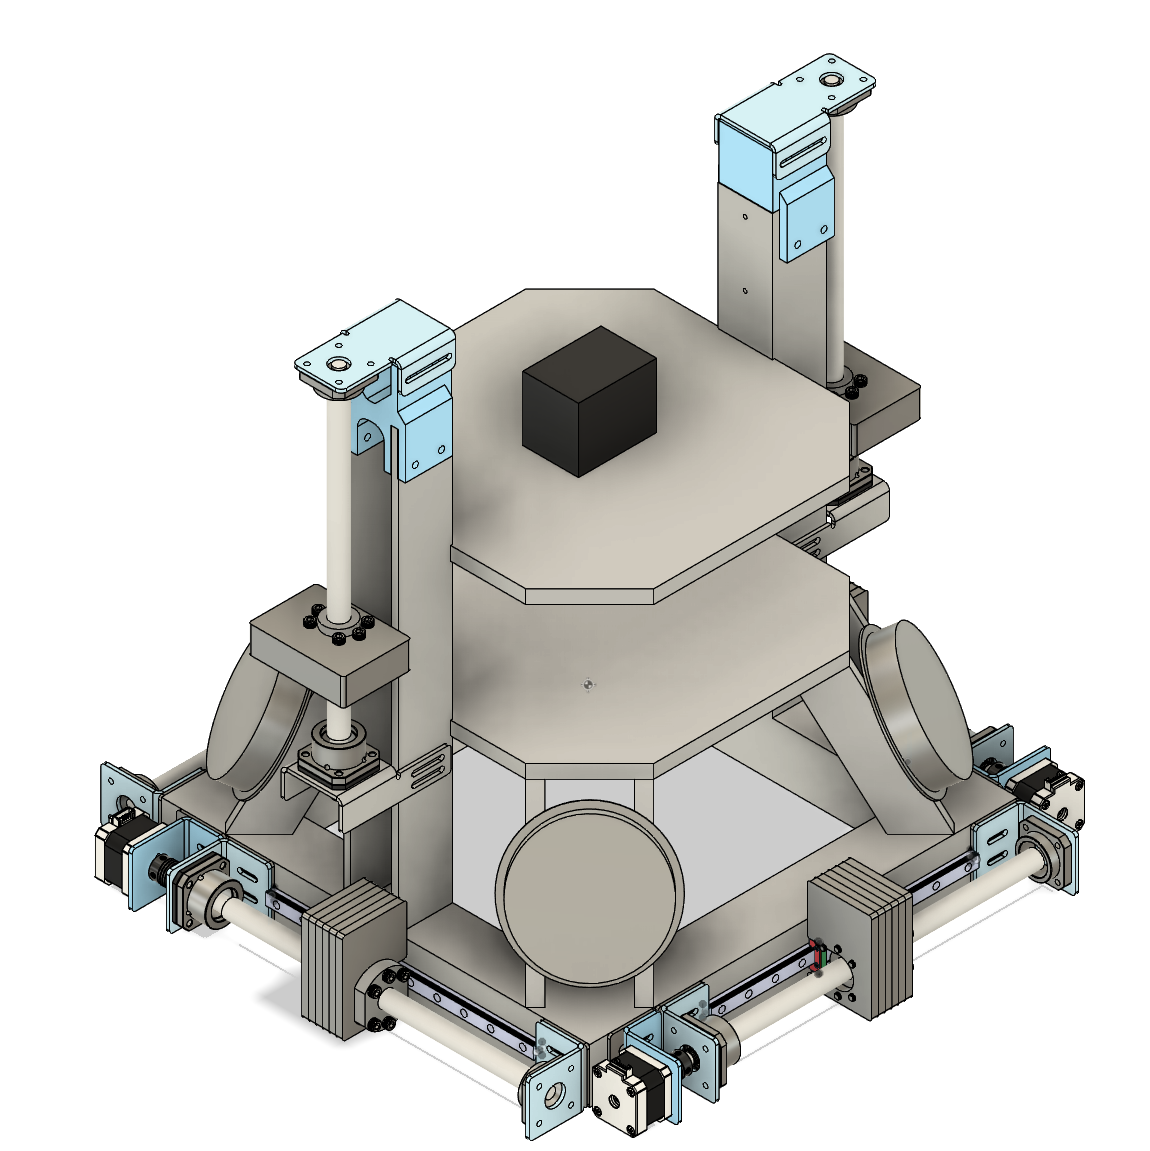
\includegraphics[width=0.95\linewidth]{figures/full_CAD.png}
    \caption{Final CAD design with all major mass contributions included, built off model completed in~\cite{gilman_automatic_2024}}
    \label{fig:final_CAD}
\end{figure}


One important aspect of the SADS when designing it's desired center of mass envelope is it's symmetrical design. \Cref{fig:final_CAD} shows the final design of the CAD model for reference. The two heaviest systems onboard are the reaction wheels and the mass balancing system itself. The pyrimdal reaction wheel configuration means the wheels contribute little horizontal inbalance. Additionally the wheels are roughly on the same horizontal plane as the platform's center of rotation, so they also contribute little verical inbalance. The main source of inbalance will thus be introduced by relatively lighter components like batteries, sensors, the flight computer, and other miscellaneous electronics.

To approximate a worst case horizontal imbalance, the heaviest of these components - the main 24V battery was placed in CAD in multiple unfavorable positions with the resulting imbalance vector in the CAD software recorded. The black prism in \Cref{fig:final_CAD} represent this battery, and it's position is placed at various edges along the top deck of the simulator. After applying a factor of safety, the resulting horizontal center of mass envelope is determined to $||\Delta\,r_x|| \approx ||\Delta\,r_x|| \approx 0.01m$. With a travel distance of $\pm100mm$ for each rail, the mass for each rail is designed as $m_i = 1.4kg$.

With the horizontal mass sizing complete, the vertical mass sizing takes a slightly different approach. Because the reaction wheels and horizontal sliding masses are positioned slightly below the center of rotation of the platform, the center of mass of the platform with with no vertical masses is biased towards $-\hat{z}_b$. The vertical masses are sized then such that when they are both in their centered postions, the vertical imbalance predicited by CAD is zero. For the vertical sliders, the designed value is $m_i = 0.65kg$. 

\subsubsection{Linear Actuator Design}

The main goal with the new linear actuator iteration is to address issues faced in \cite{gilman_automatic_2024}, where the DC motors struggled to drive the linear actuators. This issue is addressed in the new design in a variety of ways. The first is the 6V SKU-GS20173 DC motors that drive the ballscrew shaft are swapped for 24V Nema 17 stepper motors. Even though the old DC motors use a 99:1 gear ratio, the torque output of the 24V stepper motors is still more favorable at low shaft speeds. The next change is the replacement of the linear rails. On it's own, a ballscrew has one degree of rotational freedom about the shaft axis that must be restricted for it to linearly travel with no rotation. This is accomplished using a linear rail that travels along the ballscrew, and it was observed the old linear rails introduced a significant amount of friction. The new linear rails are shown and discussed further in \Cref{fig:linear_act} Finally, the ballscrew itself was found to also be introducing friction, and so each ballscrew was disassembled and serviced to reduce friction.

\begin{figure}[h]
    \centering
    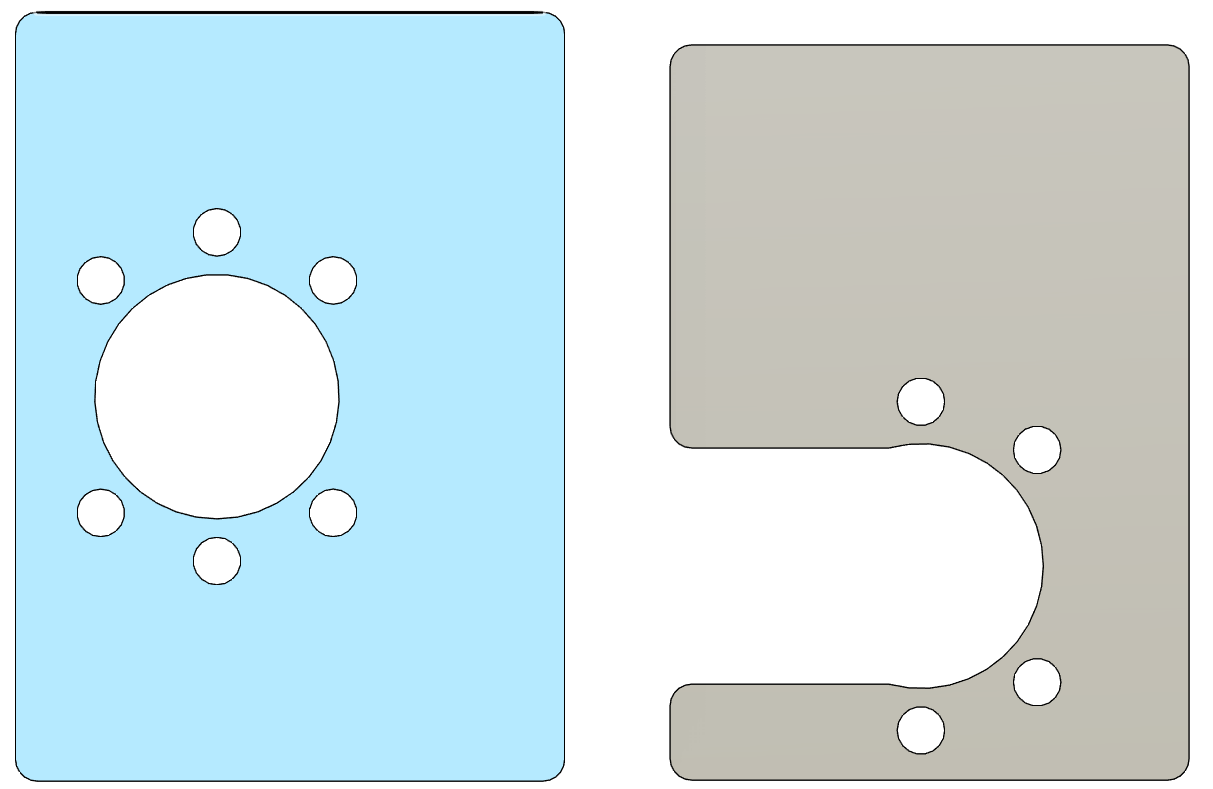
\includegraphics[width=0.8\linewidth]{figures/plate_comparison.png}
    \caption{Comparison between the previous iteration of mass plates (left) and the newly manufactured plates (right)}
    \label{fig:plate_comparison}
\end{figure}

\begin{figure}[p]
  \centering
  \begin{subfigure}[t]{0.45\textwidth}
    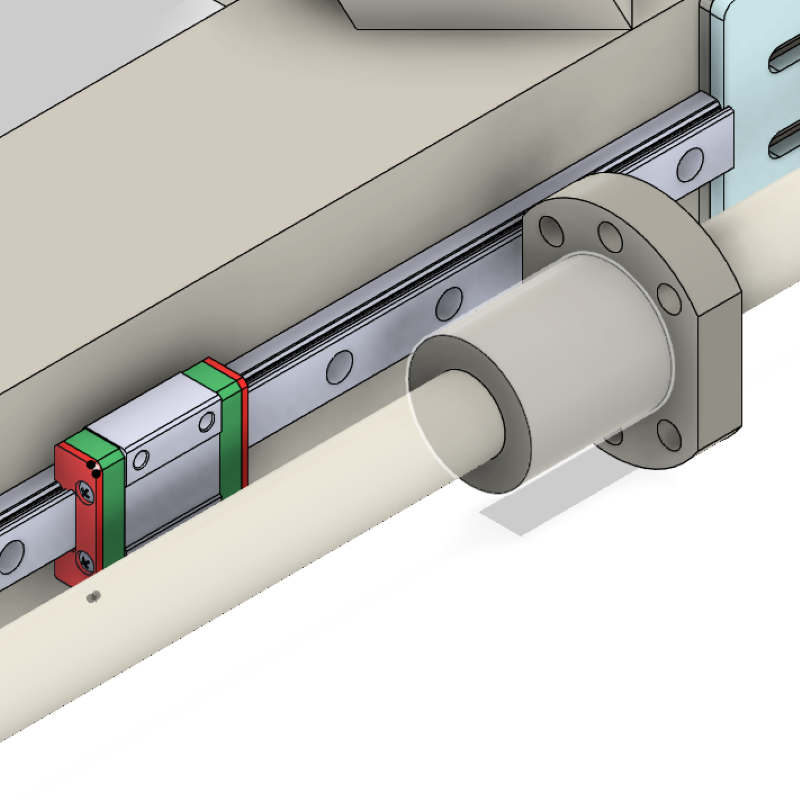
\includegraphics[width=\linewidth]{figures/linear_act_1.png}
    \caption{Assembly with just ballscrew and linear rail}
  \end{subfigure}\hfill
  \begin{subfigure}[t]{0.45\textwidth}
    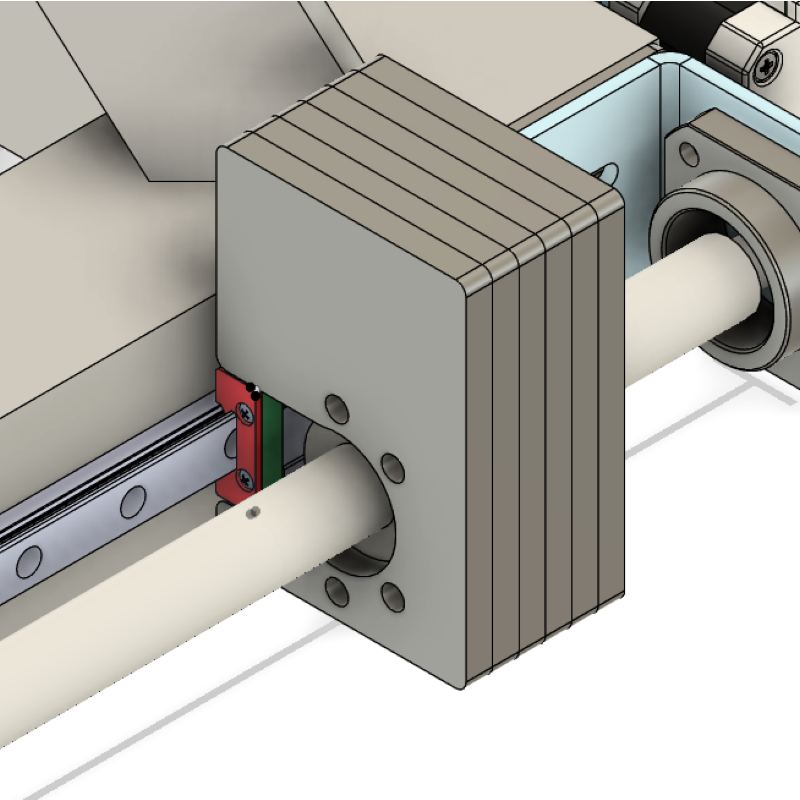
\includegraphics[width=\linewidth]{figures/linear_act_2.png}
    \caption{Assembly just before adding the final mass plate}
  \end{subfigure}
  \caption{Mass block assembly with linear rail in CAD}
  \label{fig:linear_act}
\end{figure}

\begin{figure}[p]
    \centering
    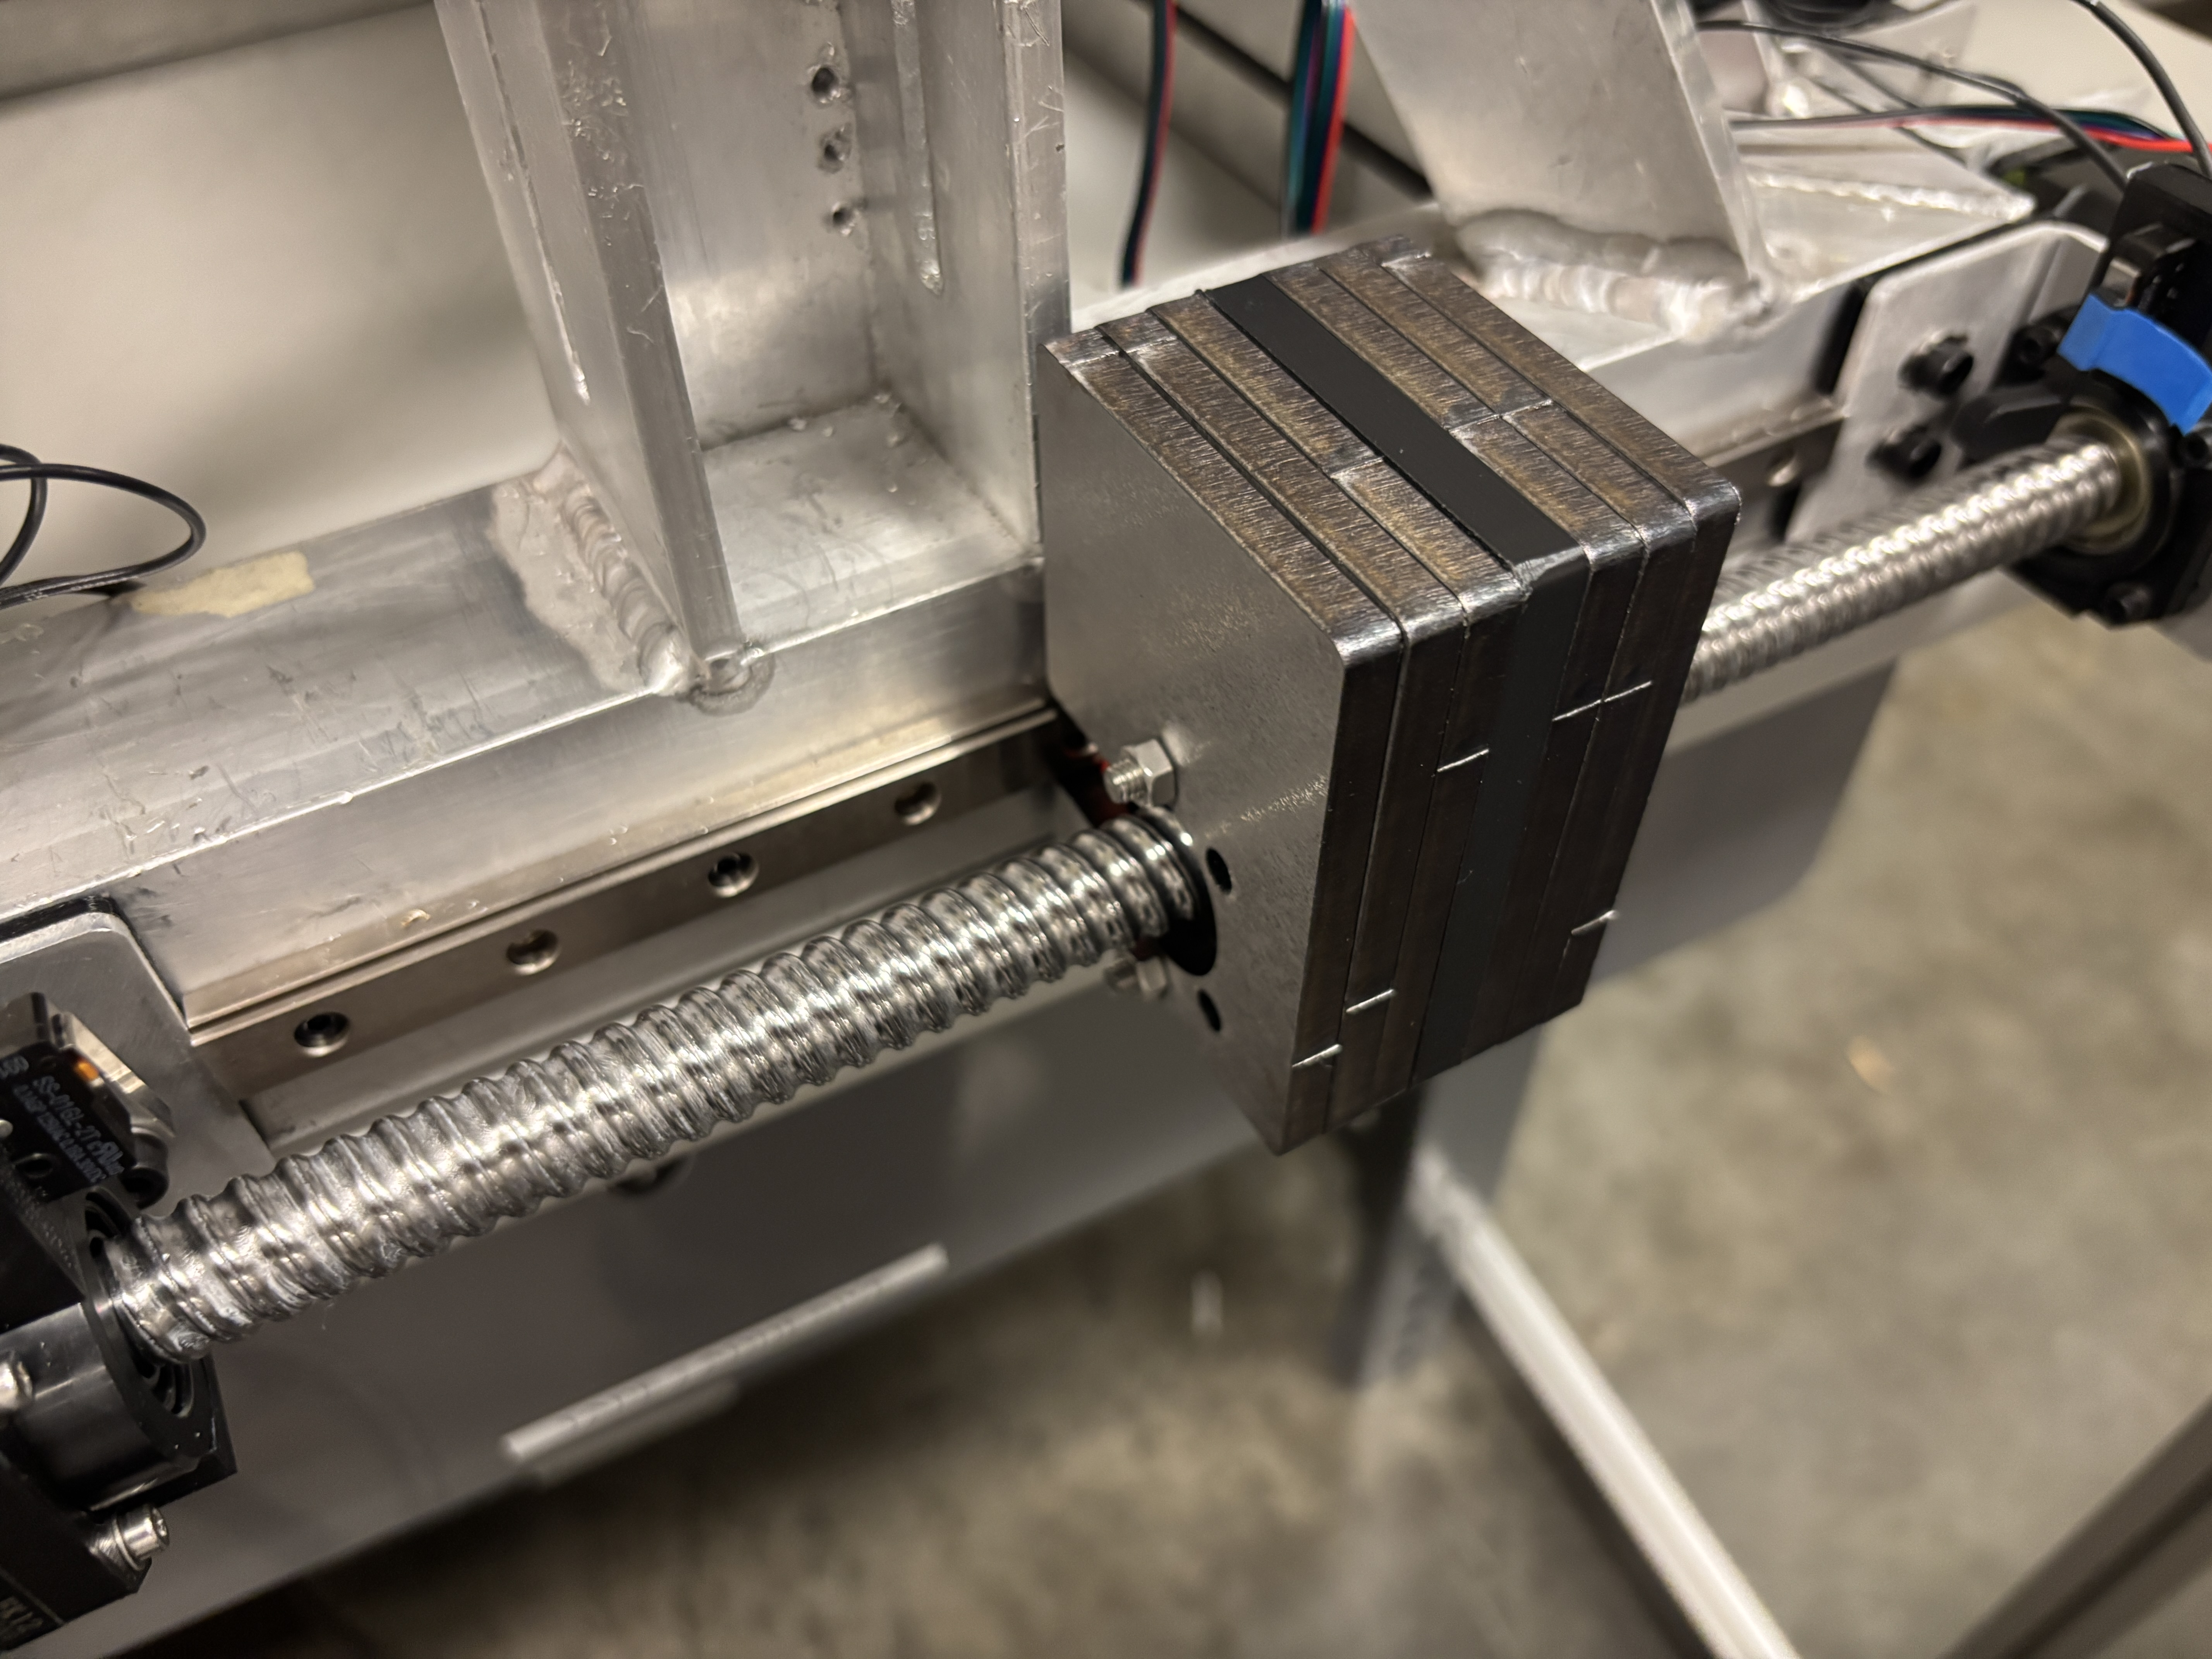
\includegraphics[width=0.85\linewidth]{figures/completed_block.jpg}
    \caption{The final mass block assembly}
    \label{fig:plate_comparison}
\end{figure}


Another issue that was quickly identified with the previous design is that to remove or install mass plates from each rail, the entire linear actuator assembly had to be disassembled. This is addressed by manufacturing a new set of mass plates, with the comparison between the two iterations shown in \Cref{fig:plate_comparison}. The most notable change is the introduction of a slot that connects the edge of the plate to the circular cutout for the ballscrew shaft. As shown in \Cref{fig:linear_act}, this allows plates to be slid directly onto the ballscrew without any disassembly. The slot is also large enough to accomodate the new linear rail, also shown in \Cref{fig:linear_act}. 

The final assembly is shown in \Cref{fig:plate_comparison}, which is completed by adding one plate with a smaller cutout slot to each end. The slot is small enough to prevent the inserted linear rail from sliding out, but still large enough to allow installation without disassembling the full system. The new assembly is verified early in the design stage via open-loop stepper motor position updates, with the exact motor control scheme discussed in the next section. The steps taken to minimize friction within the system proved to be extremely successful. In fact, the ballscrews shafts may now be turned easily by hand, even when fully loaded and integrated onto the simulator. The ability to quickly add and remove mass plates makes handling the simulator far more convenient as well.

Continuing the goals of \cite{gilman_automatic_2024}, the final design still has the additional benefit of being low cost. The ballscrews, motors, and linear rails can be easily and cheapily aquired from a growing consumer CNC market, and the new mass plates are manufactured using Cal Poly's water jet cutter.

\begin{figure}[h]
    \centering
    \includegraphics[width=0.85\linewidth,angle=-90]{figures/new_mbs_pic.jpg}
    \caption{The SADS and air bearing support with the new mass balance system integrated}
    \label{fig:new_mbs_pic}
\end{figure}

\subsection{Electrical}\label{sec:electrical}

The primary goal of the electrical design is to interface the newly developed linear actuators and an IMU to the onboard computer. An STM32F446RE was chosen as the primary onboard computer. This board has high number of GPIO pins, a maximum clock speed of 180 MHz, is low cost, and has proven compatibility with Simulink hardware suppport package. It additionally has a floating point unit that operates on 32-bit floats, which is crucial for the rapid matrix multiplication needed to propagate a Kalman filter in realtime. Despite these benefits, using a microcontroller still has numerous drawbacks, the main one being the need to reflash the board to switch bewteen programs. In the final iteration of the SADS, the onboard computer ideally runs as a Linux-based RTOS, where the operator can easily load and switch between multiple programs. Future work for the onboard computer is discussed further in \Cref{chap:conclusion}.

\begin{figure}[h]\label{fig:wiring}
    \centering
    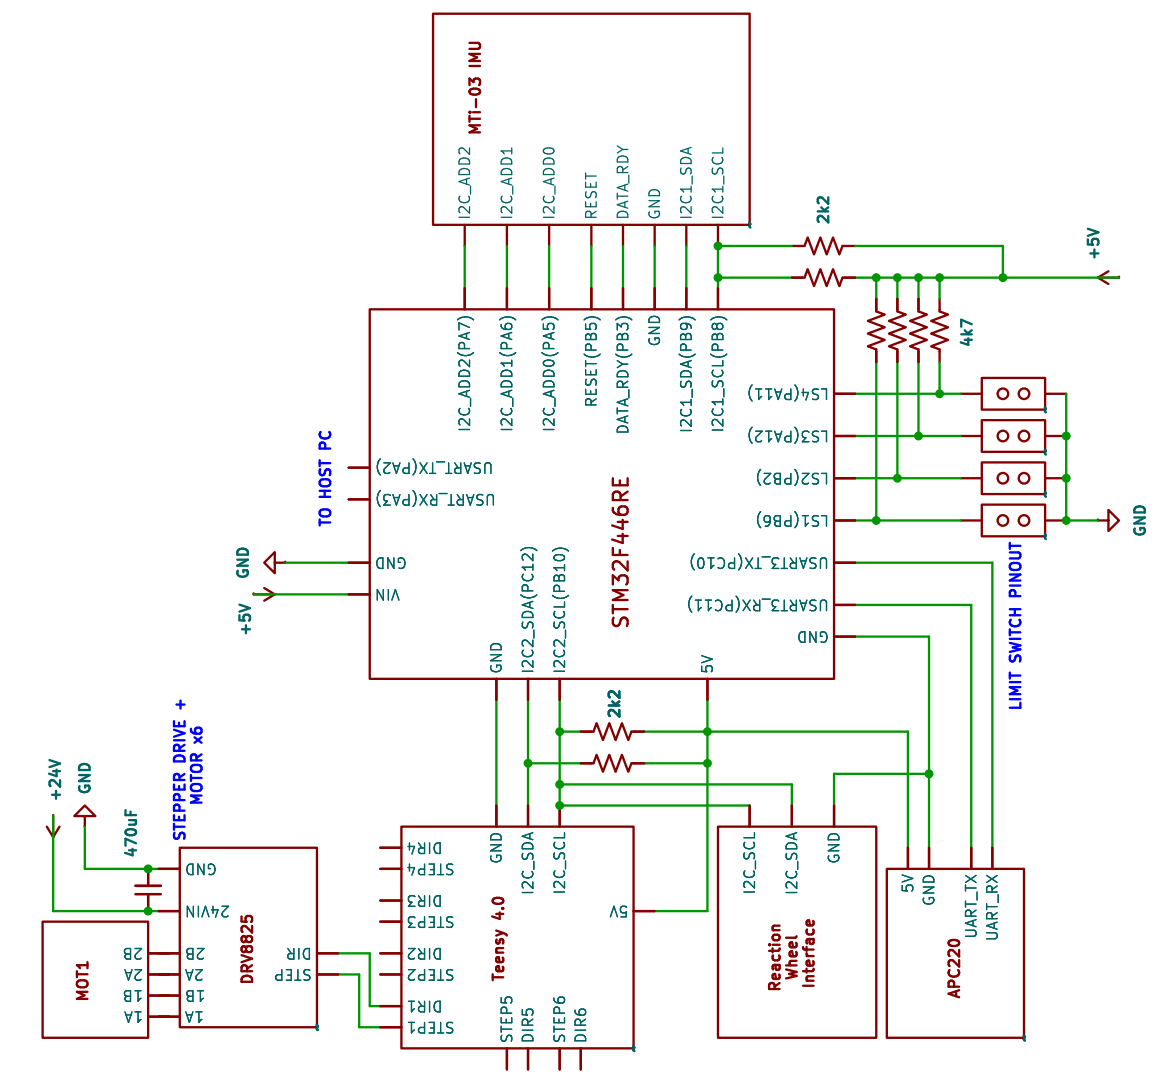
\includegraphics[width=\linewidth,angle=-90]{figures/wiring.png}
    \caption{Wiring schematic}
\end{figure}

The MTi-03 was chosen as the IMU for it's noise characteristics and easy of integration with the STM32. The MTi-03 has a noise density of $0.003\si{\degree\per\second\per\Hz^{1/2}}$, which is favorable when compared to the values found on existing balancing systems as shown in \Cref{table:existing_testbeds}. The IMU and onboard computer communicate over I2C, with more detail provided in \Cref{sec:software}.

Each stepper motor is controlled by a DRV8825 motor driver. The driver advances the motor one step per pulse of the STEP pin. The amount of steps required for one full revolution of the shaft is customizable on the DRV8825, but lower values were observed to cause intense vibrations when integrated on the platform. The minimum value that ensured smooth operation was found to be 3200 steps per revolution. Additionally, early simulation results suggested the mass blocks may have to travel as fast as 15\si{\mm\per\second} during active balancing. Since the ballscrews advance at 10\si{mm} per revolution, this means the onboard computer will need to generate a maximum of 4800 steps per second per motor. Generating steps at this rate on the STM32 caused timing issues with other tasks such as I2C communications and filter propagatation. To take load off the STM32, it sends the desired shaft position of each motor to a seperate Teensy 4.1 over I2C. The Teensy then handles all of the required step generation.

The final two interfaces with the onboard computer are the APC220 and reaction wheel interface. The APC220 communicates over UART with the STM32 to send telemetry wirelessly to a host PC. Since the simulator has full rotational freedom about yaw, telemetry during live airbearing tests cannot be sent through a wired connection. The reaction wheel interface communicates over I2C with the STM32 which accepts wheel speed commands. Reaction wheel control is disccused in \cite{nalley2025development}. \Cref{fig:wiring} shows a simplifed wiring diagram of the system including all of the boards discussed here.

\begin{figure}[h]\label{fig:OBC}
    \centering
    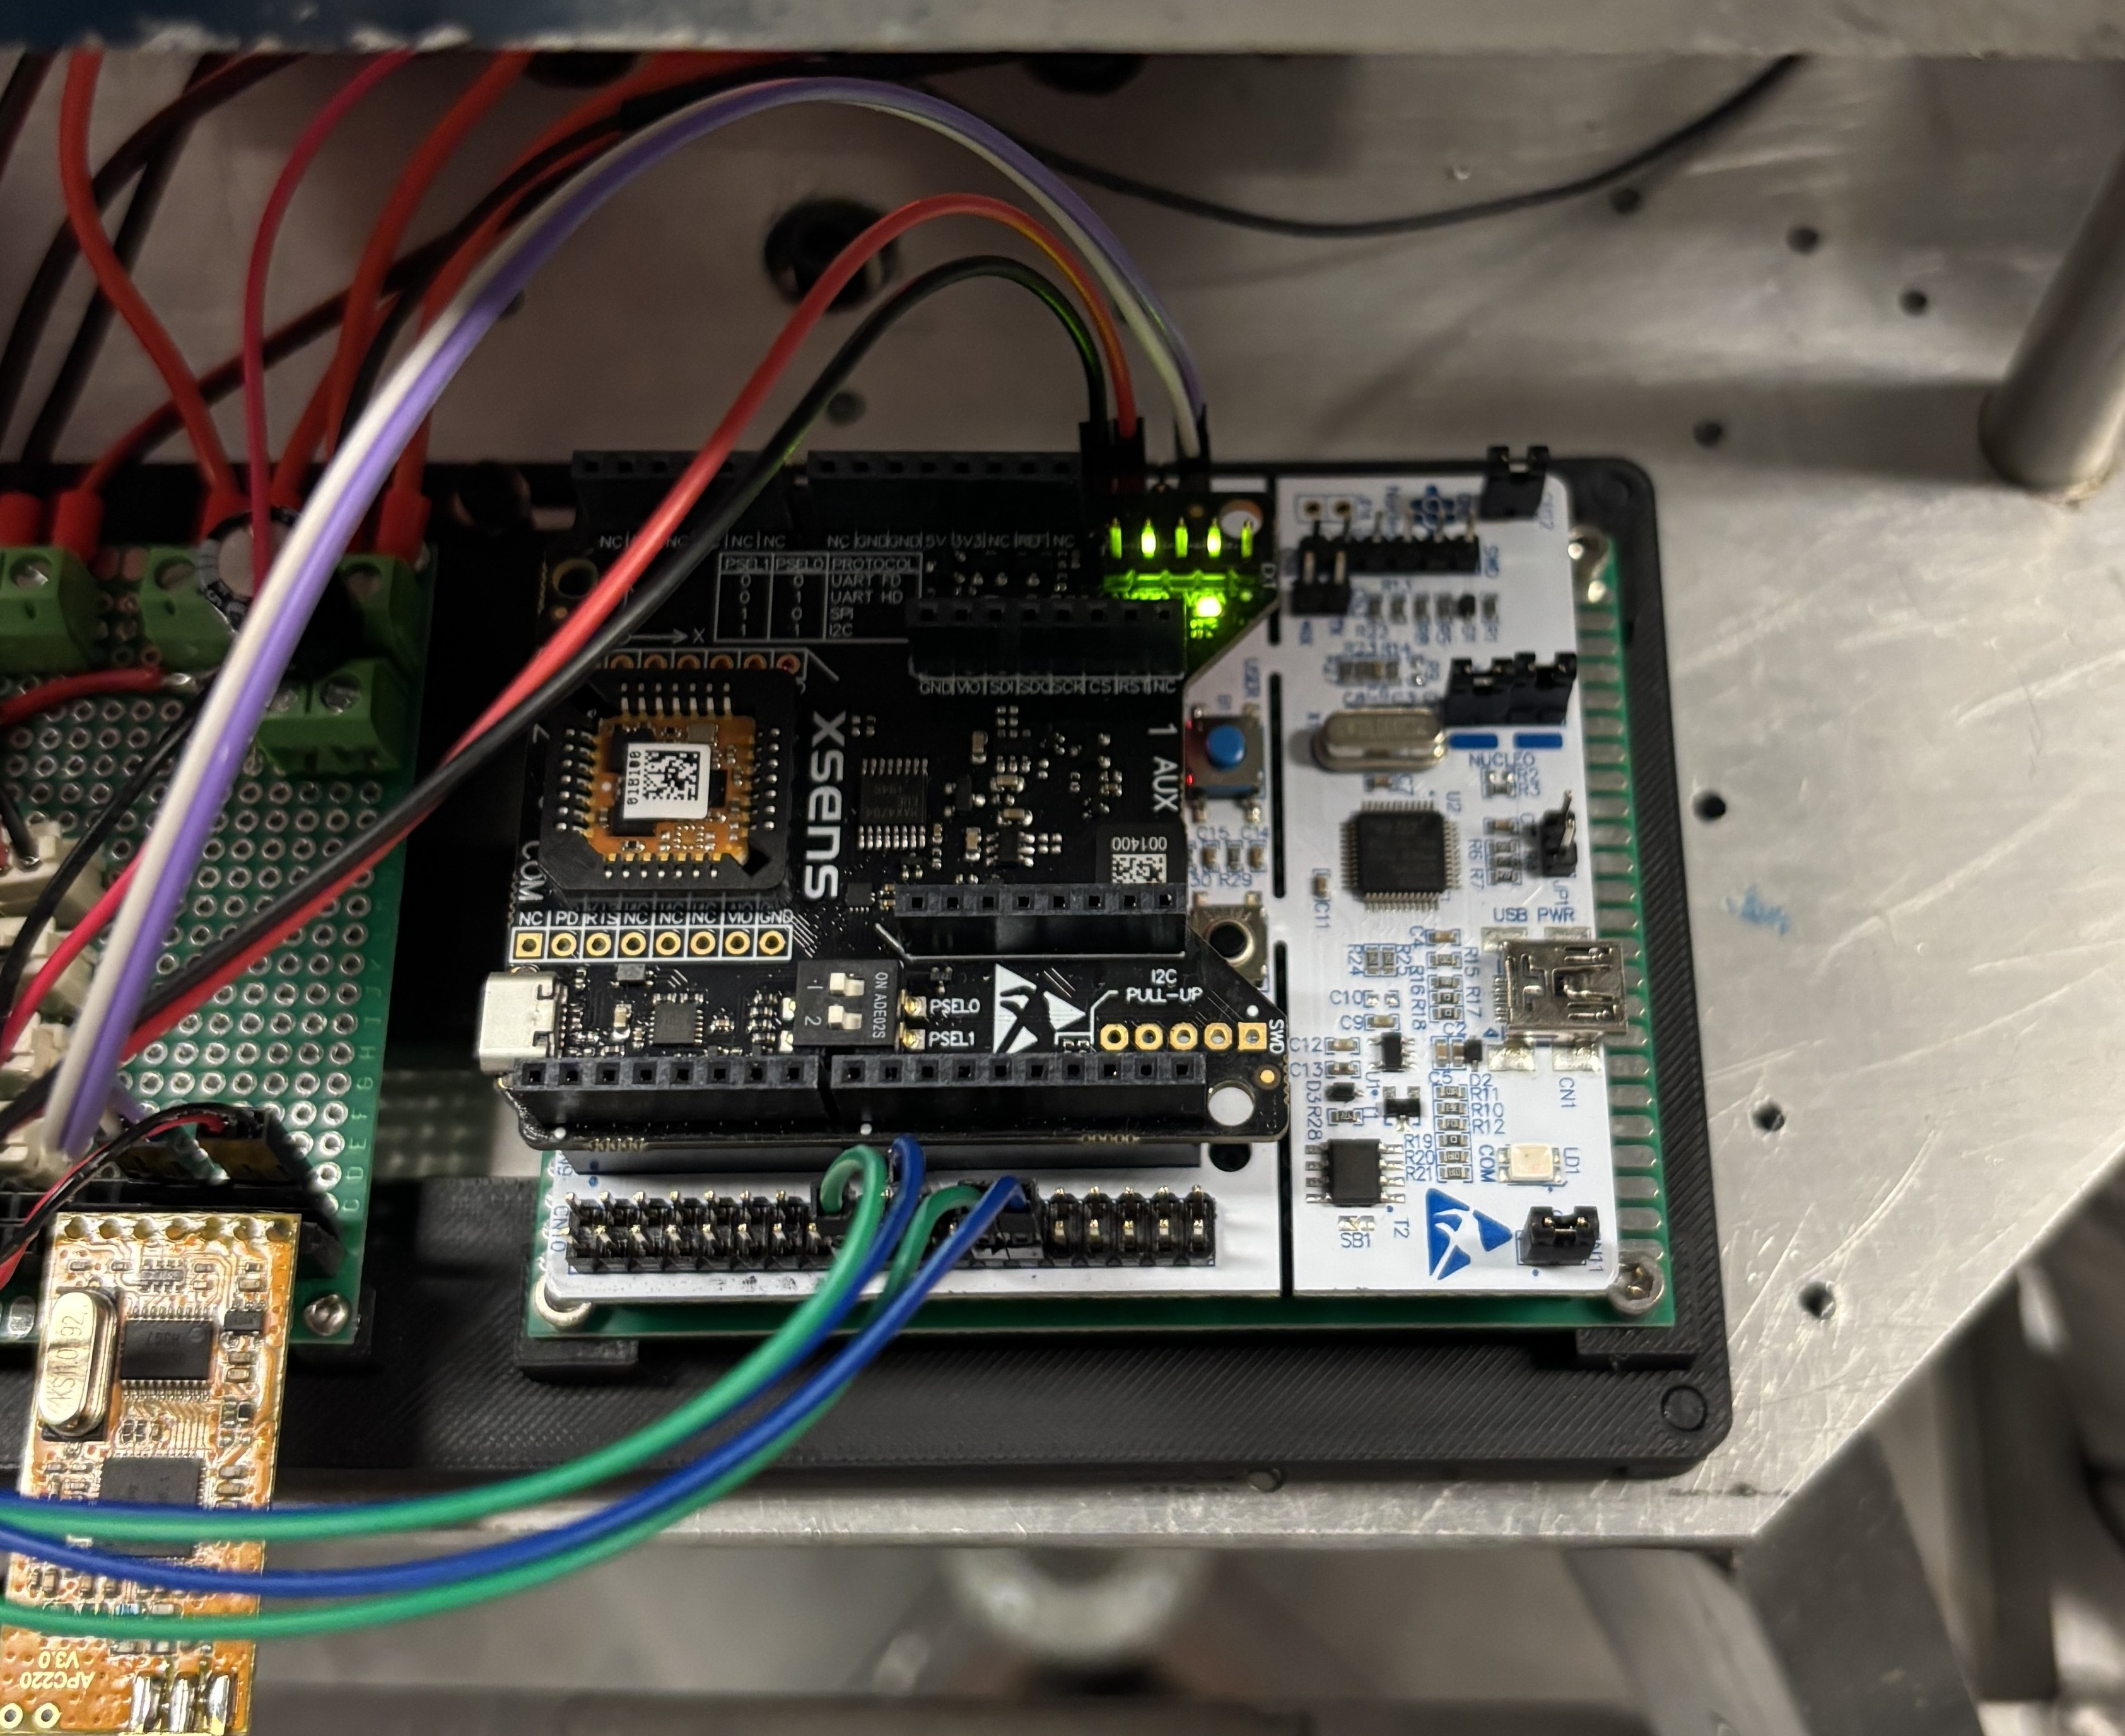
\includegraphics[width=0.80\linewidth]{figures/OBC.jpg}
    \caption{The STM32F446RE, MTi-03, and APC220 (bottom left) integrated onto the simulator}

\end{figure}

\subsection{Software}\label{sec:software}

The goal of the software design is to utilize Simulink Coder with the STM32 to make the implementation of the discussed balancing algorithms simpler. For this method to be viable, the Simulink model must interface with the external boards in the system as disccused in \Cref{sec:electrical}. 

\begin{figure}
    \centering
    \usetikzlibrary{arrows.meta,positioning,fit,calc,shapes.misc}
\usetikzlibrary{shapes.geometric}

\begin{tikzpicture}[
    scale=0.63,                        % <-- change this to resize (e.g., 0.8 or 1.3)
    every node/.style={transform shape},
    node distance=2em and 4em,
    line/.style={-Latex},
    block/.style={
        rectangle, draw, rounded corners,
        fill=blue!15, align=center,
        minimum width=11em, minimum height=5em
    },
    smallblock/.style={
        rectangle, draw, rounded corners,
        fill=blue!10, align=center,
        minimum width=10em, minimum height=2.5em
    },
    tallblock/.style={
        rectangle, draw, rounded corners,
        fill=blue!10, align=center,
        minimum width=10em, minimum height=8em
    },
    extbox/.style={rectangle, draw, dashed, rounded corners=8pt, inner sep=6pt},
    callout/.style={font=\footnotesize, midway, fill=white, inner sep=1pt}
]

% -------------------- LEFT EXTERNAL (IMU) --------------------


\node[smallblock,  yshift=-5ex,fill=white]  (p_status) {Pipe Status};
\node[smallblock, yshift=5ex,fill=white]  (meas_pipe) {Measurement Pipe};
\node[extbox, fit=(p_status)(meas_pipe),label={[align=center]above:\large{\textit{MTi-03 IMU}}}] (imu) {}; 
% -------------------- MAIN SYSTEM --------------------
\node[tallblock, right=of p_status,xshift=8ex,yshift=5ex] (driver) {MTi Driver\\ Matlab System Object};
\node[smallblock, above=of driver, yshift=4ex] (xbus) {Xbus Library};
\node[block, right=of driver,xshift=6.5ex,fill=orange!25] (ekf) {Extended Kalman\\Filter};
\node[block, below=of ekf,xshift=8ex,yshift=-10ex,fill=orange!25] (ctrl) {Control Law};
\node[block, left=of ctrl,fill=orange!25] (alloc) {Mass Slider\\Allocation};

\node[block,fill=white] (stepper) at ($(p_status |- alloc)$){Stepper Motor\\ Control System};


% -------------------- CONNECTIONS --------------------
\draw[line] (meas_pipe.east) -- 
    node[above,font=\footnotesize, align=center, text width=15ex] {XBus Meas. Messages}
($(driver.west |- meas_pipe.east)$);

\draw[line] ($(driver.west |- p_status.east)$) -- 
    node[below,font=\footnotesize, align=center, text width=15ex] {Request Pipe Status}
(p_status.east);

\draw[line,Latex-Latex] (xbus) -- 
    node[fill=white,font=\footnotesize] {Function calls}
(driver);

\draw[line] (driver) -- 
    node[above,font=\footnotesize, align=center, text width=15ex] {Gyro +\\Accelerometer}
(ekf);

\coordinate (ekfOut1) at ($(ekf.east)+(0em,1em)$);
\coordinate (ekfWrap1) at ($(ekfOut1)+(9em,0)$);   % distance right; tweak 4em as you like

\coordinate (ekfOut2) at ($(ekf.east)+(0em,-1em)$);
\coordinate (ekfBranch) at ($(ekfOut2)+(7em,-6em)$);   % distance right; tweak 4em as you like

\draw[line] (ekfOut1) -- 
    node[above, align=center,xshift=-7ex,font=\large] {$\bm{q}$, $\bm{\omega}$}
(ekfWrap1) |- ($(ctrl.east)+(0,-1.1em)$);
\draw[line] (ekfOut2) -| 
    node[below,xshift=-13ex,font=\large] {$\bm{g}$}
(ekfBranch) |- ($(ctrl.east)+(0,+1.1em)$);
\draw[line] (ekfBranch) -| (alloc);
\draw[line] (ctrl) --
    node[above, align=center,font=\large] {$\bm{\tau}_c$}
(alloc);
\draw[line] (alloc) -- 
    node[above, align=center,xshift=5ex,font=\large] {$\Delta\bm{d}$} 
(stepper);

% Boundary box for Simulink model
\node[extbox, fit=(xbus)(driver)(ekf)(ctrl)(alloc)(ekfWrap1),
    label={[align=center]above:\Large{\textit{Simulink Embedded Model}}}] (simbox) {};

\node[draw, fill=orange!25, rounded corners,above=of meas_pipe,yshift=15ex] (sim) {MATLAB/Simulink Components};
\node[draw, fill=blue!15, below=of sim, rounded corners,yshift=3ex] (c) {C/C++ Components};

\end{tikzpicture}
    \caption{Functional software architecture during balancing}
    \label{fig:software_flowchart}
\end{figure}

The most of challenging of these is the MTi-03 IMU, which communicates using the XBus communication protocol. The MTi-03 has various data pipes depending on which address is read over I2C. In nominal operations, the IMU collects measurement data and sends it to the measurement pipe, which operates as a first-in first-out buffer. The amount of data in this buffer is stored in the pipe status address. For each new measurement, the onboard computer must first request the pipe status, read the proper amount of bytes from the measurement pipe, and finally unpack the raw XBus message into gyroscope and accelerometer readings. 

To aid users, the manufacturer Movella provides an XBus library which has numerous functions to aid in this process. Because the library is written in C/C++, a MATLAB System Object is developed which bridges the gap between the XBus library and the standard MATLAB/Simulink environment. The primary data flows within the software are shown in \Cref{fig:software_flowchart}. Once the System Object outputs the raw gyroscope and accelerometer into the model, the majority of the remaining computation occurs in the MATLAB/Simulink environment. The high amout of matrix and vector manipulation within the EKF and control laws makes this environment preferrable to C/C++. 

In addition to the Embedded Simulink model, a seperate configuration program was written C. In this program the operator communicates with the STM32 on a host PC in a terminal-like environment over UART. The program allows various system parameters to be configured like the MTi-03 sample rate and sliding mass homing positions. Debugging system issues here is also far more convenient than the Simulink model since the STM32 can print out debug telemetry in the terminal.

\subsection{Algorithm Implementation}

\subsubsection{Onboard Filtering for Attitude Determination}

For most balancing methods, the onboard computer must calculate a value for $\bm{q}$ in real-time. To accomplish this, an Extended Kalman Filter is implemented in the MATLAB/Simulink environment which is then autocoded and deployed on the STM32. The goal of this filter is to propagate the state forward using the gyroscope output, and correct it with the accelerometer. The onboard EKF state then is simply $\bm{x} = \bm{q}$. If a balancing algorithm requires a value for $\bm{\omega}$, the gyroscope output is used. The state is propagated using
\begin{equation}\label{equation:EKF_process}
    \bm{x}_k^-=\bm{x}_{k-1} + T\begin{bmatrix}
    
    -\frac{1}{2}\bm{\epsilon}_{k-1}^T\bm{\omega}_{k-1} \\
    \frac{1}{2}(\eta_{k-1}\mathbb{1} +
    \bm{\epsilon}_{k-1}^{\times})\bm{\omega}_{k-1}
\end{bmatrix}
\end{equation}
where $\bm{x}_k^-$ is the predicted state, and $\bm{\omega}$ is taken directly from the gyroscope readings. Next, the state is corrected using the accelerometer reading, where the accelerometer output is treated as a measurement for $\bm{g}_b$. Measurements are predicted using 
\begin{equation}\label{equation:EKF_meas}
    \hat{\bm{y}}_k^-=
    \begin{bmatrix}    
    \eta_k^-\mathbb{1}-(\bm{\epsilon}_k^-)^{\times} & -\bm{\epsilon}_k^-
    \end{bmatrix}
    \begin{bmatrix}    
    \bm{g}^\mathcal{N} & (\bm{g}^\mathcal{N})^{\times} \\
    \bm{0} & - (\bm{g}^\mathcal{N})^T
    \end{bmatrix}
    \begin{bmatrix}    
    \eta_k^- \\
    \bm{\epsilon}_k^-
    \end{bmatrix}
\end{equation}
where $\eta_k^-$ and $\bm{\epsilon}_k^-$ are taken from $\bm{x}_k^-$, and $\bm{g}^\mathcal{N}=[0, 0,-9.81]^T$

In reality, unless the accelerometer is perfectly aligned with the simulator's center of rotation, the sensor output will include the effects of centrepital acceleration. However, since the MTi-03 IMU is mounted close to the center of rotation on the SADS and the body rates of the simulator during balancing are low, the effects of centrepital acceleration are not included in the measurement model.

Following the standard EKF formulation, the process and measurement Jacobians are computed. \Cref{equation:EKF_process} is linearized about $\bm{x}_{k-1}$, while \Cref{equation:EKF_meas} is linearized about $\bm{x}_k^-$. The process Jacobian $\bm{F}$ and measurement Jacobian $\bm{H}$ are 
\begin{equation}
    \bm{F}_k = \mathbb{1}+
\begin{bmatrix}
0 & -\tfrac{1}{2}\bm{\omega}_{k-1}^{T}\\[3pt]
\tfrac{1}{2}\bm{\omega}_{k-1} & -\tfrac{1}{2}\bm{\omega}_{k-1}^{\times}
\end{bmatrix}.
\end{equation}

\begin{equation}
\bm{H}_k =
\begin{bmatrix}
2\!\left(\eta_k^- \mathbb{1} - (\bm{\epsilon}_k^-)^{\times}\right)\bm{g}^{\mathcal N}
\\
-2\,\bm{g}^{\mathcal N}(\bm{\epsilon}_k^-)^{\!T}
+2\!\left((\bm{\epsilon}_k^-)^{\!T}\bm{g}^{\mathcal N}\right)\mathbb{1}
+2\,\bm{\epsilon}_k^- (\bm{g}^{\mathcal N})^{\!T}
+2\,\eta_k^- (\bm{g}^{\mathcal N})^{\times}
\end{bmatrix}^T.
\end{equation}
With $\bm{F}$ computed, the filter propagates the covariance forward using
\begin{equation}
        \bm{P}_k^- = \bm{F}_{k-1}\bm{P}_{k-1}\bm{F}_{k-1}^T + \bm{L}\bm{Q}\bm{L}^T
\end{equation}
where $\bm{Q}$ is the tunable process noise matrix, and $\bm{L}$ relates the process noise to the state and is defined as
\begin{equation}
    \bm{L} = T\begin{bmatrix}
        0      & \bm{0} \\
        \bm{0} & \mathbb{1}_{3\times3}
    \end{bmatrix}\in\mathbb{R}_{4\times4}
\end{equation}
Next the Kalman gain $\bm{K}$ is computed with
\begin{equation}
    \bm{K}_k = (\bm{P}_k^-\bm{H}_k^T)/(\bm{H}_k\bm{P}_k^-\bm{H}_k^T + \bm{R})
\end{equation}
where $\bm{R}$ is the tunable measurement noise matrix.

The filter iteration ends with the state and covariance being corrected using the Kalman gain as follows
\begin{equation}
    \bm{x}_k = \bm{x}_k^- + \bm{K}(\bm{y}_{\text{meas}}-\hat{\bm{y}}_k^-)
\end{equation}
\begin{equation}
    \bm{P}_k = (\mathbb{1} - \bm{K}_k\bm{H}_k)\bm{P}_k^-(\mathbb{1} - \bm{K}_k\bm{H}_k)^T
    + \bm{K}_k\bm{R}\bm{K}_k^T
\end{equation}
where $\bm{y}_{\text{meas}}$ is the accelerometer reading. At this point the quaternion is normalized using $\bm{x}_k = \bm{x}_k / ||\bm{x}_k||$ and is sent along with $\bm{g}_b$ to the control law, with $\bm{g}_b$ being computed from \Cref{equation:C_from_q}.

The filter as described here still has room for improvement. Including an estimate of the gyroscope bias in the state vector would improve accuracy over longer runs, and there are more sophisticated methods to enforcing a unit norm for $\bm{q}$. However the filter's simulated performance as described in \Cref{sec:sim_setup} proved to be adequate for mass balancing, so improvements to the filter are left as future work with more detail described in \Cref{chap:conclusion}.

\subsubsection{Passive Balancing Operation}

With the EKF implemented, passive balancing becomes relatively simple. The operator manually sets the initial attitude of the simulator and begins recording telemetry. The simulator tumbles either freely or under the influence of the open loop reaction wheel commands depending on balancing method being used. The reaction wheel interface is additionally able to feedback the recorded torque which is bundled with the telemetry. 

The attitude, body rates, and reaction wheel torques are loaded onto the host PC. The data is post processed and inputted into either the UKF or the least-squares estimator depending on the algorithm. Both the UKF and least-squares estimator are implemented in MATLAB directly mirroring the equations as laid out in \Cref{sec:LSR} and \Cref{sec:UKF}. For the batch estimation algorithm, the discrete-time integrals are handled through trapezoidal integration. The resulting estimate for $\bm{r}$ is converted into a set of new mass positions $\Delta{r}$, which are finally applied through the stepper motors. This process is repeated until the estimates converge, with the exact conditions for convergence being discussed further in \Cref{chap:results}. 

\begin{figure}
    \centering
    \usetikzlibrary{arrows.meta,positioning,fit,calc,shapes.misc}
\usetikzlibrary{shapes.geometric,quotes}

\begin{tikzpicture}[
  scale=0.64,
  every node/.style={transform shape},
  line/.style={draw, -Latex, thick, rounded corners=4pt},
  box/.style={rectangle, draw, rounded corners, align=center, fill=white,
              minimum width=16em, minimum height=4em},
  smallbox/.style={rectangle, draw, rounded corners, align=center, fill=white,
              minimum width=14em, minimum height=3.5em},
  extbox/.style={rectangle, draw, dashed, rounded corners=8pt, inner sep=6pt}
]

% =======================================================
%                     MAIN COMPONENTS
% =======================================================
\node[box] (stm32) at (0,0) {STM32 Microcontroller};
\node[smallbox] (mti) [above=of stm32, yshift=2.5em] {MTi-03 IMU};

\coordinate (telem_out) at ($(stm32.south)+(4em,0em)$);
\coordinate (fc_in) at ($(stm32.south)+(-4em,0em)$);
\node[smallbox,minimum width=9em] (apc) [below=of telem_out, yshift=-2em] {APC220 Radio\\Module};
\node[smallbox,minimum width=9em] (rwi) [left=of stm32, xshift=-7em] {Reaction Wheel\\Interface};

% Teensy subsystem (right side)

\node[smallbox,minimum width=9em,right = of stm32,xshift=19ex] (teensy)  {Teensy 4.0};
\node[smallbox,minimum width=9em,below = of teensy,yshift=-4ex] (drv) {DRV8825 Drivers};
\node[smallbox,minimum width=9em,below = of drv,yshift=-4ex] (steppers) {Stepper Motors};

% Host PC subsystem (left bottom)

\node[smallbox,below left=of stm32,xshift=-5ex,yshift=-25ex] (matlab) {Batch Estimation\\ Algorithm MATLAB};
\node[smallbox, above = of matlab,yshift=3ex] (fc)  {Flight Code\\C/C++ Source};
% =======================================================
%                     CONNECTIONS
% =======================================================

% IMU → STM32
\draw[line] (mti.south) -- 
node[fill=white, font=\footnotesize]  {Gyro + Accelerometer Readings -- I2C}
(stm32.north);

% Reaction Wheel Interface ↔ STM32
\coordinate (wheel_out) at ($(stm32.west)+(0em,0.6em)$);
\coordinate (torque_in) at ($(stm32.west)+(0em,-0.6em)$);
\draw[line] (wheel_out) --  
  node[above, font=\footnotesize,align=center, text width=20ex] {Commanded Wheel Speeds -- I2C} 
($( rwi.east |- wheel_out)$) ;
\draw[line] ($( rwi.east |- torque_in)$) --
  node[below, font=\footnotesize,align=center, text width=20ex] {Measured Torque -- I2C} (torque_in);

% STM32 → Teensy (Commanded Mass Positions)
\draw[line] (stm32.east) -- 
  node[above, font=\footnotesize, pos=0.4,align=center,text width = 17ex] {Commanded Mass Positions -- I2C} 
(teensy.west);

% Teensy downward chain
\draw[line] (teensy.south) -- node[fill=white, font=\footnotesize]
  {Step Generation} (drv.north);
\draw[line] (drv.south) -- node[fill=white, font=\footnotesize]
  {Positional Control} (steppers.north);

% Host PC internal (Simulink → Flight Code)
\draw[line] (matlab.north) -- 
  node[fill=white, font=\footnotesize] {Estimated Center of Mass} 
(fc.south);

% Host PC → STM32 (USB upload)
\draw[line] (fc.east) -|
  node[align=center, text width=15ex,above, font=\footnotesize, pos=0.3] {Compiled Flight\\Code -- USB} 
(fc_in);

% STM32 → APC220 (UART telemetry)
\draw[line] (telem_out) -- 
    node[font=\footnotesize,fill=white] {Telemetry -- UART} 
(apc.north);

% Telemetry RF (Host PC → APC)
% \coordinate (rfbus) at ($(stm32.south)+(0,-4)$);
% \draw[line] (matlab.east) -- node[above, font=\footnotesize]
%   {Telemetry -- RF} (rfbus -| matlab.east) -- (rfbus -| apc.south);
% \draw[line] (rfbus -| apc.south) -- (apc.south);
\draw[line] (apc.south) |- 
    node[fill=white,pos=0.2,font=\footnotesize]{Telemetry -- RF}
(matlab.east);

\node[extbox, fit=(fc)(matlab), label={[align=center]above:Host PC}] (host) {};
\node[extbox, fit={(teensy)(drv)(steppers)}, label={[align=center]above:Stepper Motor\\Control System}] (teensybox) {};

\end{tikzpicture}
    \caption{Primary data flows and components during passive balancing}
    \label{fig:sys_arch_passive}
\end{figure}

\subsubsection{Active Balancing Operation}

For active balancing, the values computed by the EKF are inputted into the various control laws described \Cref{Sec:active_methods}. The control laws output a desired torque, which is converted into a desired change in center of mass according to \Cref{equation:torque_to_del_r}, and then further converted into a change of sliding mass positions according to \Cref{equation:delta_d_sol}. The benefits of offloading step generation to the Teensy are again seen here, as the controller ends each timestep by simply performing a small I2C write with the desired positions of each motor. The task of implementing step generation in the Simulink model is entirely avoided. 

To run the an active balancing operations, the proper Simulink model is compiled on the host PC and flashed onto the STM32 over USB. The USB is disconnected and the feedback control is activated via button press. The simulator automatically balances, and the operator ends the test when the sliding mass positions converge. The conditions for sliding mass convergence are also discussed in \Cref{chap:results}.Telemetry may still be sent over the APC220 to help with plotting results and debugging issues, but is not strictly necessary for the procedure. 


\begin{figure}
    \centering
    \usetikzlibrary{arrows.meta,positioning,fit,calc,shapes.misc}
\usetikzlibrary{shapes.geometric,quotes}

\begin{tikzpicture}[
  scale=0.64,
  every node/.style={transform shape},
  line/.style={draw, -Latex, thick, rounded corners=4pt},
  box/.style={rectangle, draw, rounded corners, align=center, fill=white,
              minimum width=16em, minimum height=4em},
  smallbox/.style={rectangle, draw, rounded corners, align=center, fill=white,
              minimum width=14em, minimum height=3.5em},
  extbox/.style={rectangle, draw, dashed, rounded corners=8pt, inner sep=6pt}
]

% =======================================================
%                     MAIN COMPONENTS
% =======================================================
\node[box] (stm32) at (0,0) {STM32 Microcontroller};
\node[smallbox] (mti) [above=of stm32, yshift=2.5em] {MTi-03 IMU};

\coordinate (telem_out) at ($(stm32.south)+(4em,0em)$);
\coordinate (fc_in) at ($(stm32.south)+(-4em,0em)$);
\node[smallbox,minimum width=9em] (apc) [below=of telem_out, yshift=-2em] {APC220 Radio\\Module};
% \node[smallbox,minimum width=9em] (rwi) [left=of stm32, xshift=-7em] {Reaction %Wheel\\Interface};

% Teensy subsystem (right side)

\node[smallbox,minimum width=9em,right = of stm32,xshift=19ex] (teensy)  {Teensy 4.0};
\node[smallbox,minimum width=9em,below = of teensy,yshift=-4ex] (drv) {DRV8825 Drivers};
\node[smallbox,minimum width=9em,below = of drv,yshift=-4ex] (steppers) {Stepper Motors};

% Host PC subsystem (left bottom)

\node[smallbox,below left=of stm32,xshift=-5ex,yshift=-25ex] (matlab) {Plotting / Debug};
\node[smallbox, above = of matlab,yshift=3ex] (fc)  {Embedded Simulink Model};
% =======================================================
%                     CONNECTIONS
% =======================================================

% IMU → STM32
\draw[line] (mti.south) -- 
node[fill=white, font=\footnotesize]  {Gyro + Accelerometer Readings -- I2C}
(stm32.north);

% Reaction Wheel Interface ↔ STM32
% \coordinate (wheel_out) at ($(stm32.west)+(0em,0.6em)$);
% \coordinate (torque_in) at ($(stm32.west)+(0em,-0.6em)$);
% \draw[line] (wheel_out) --  
%   node[above, font=\footnotesize,align=center, text width=20ex] {Commanded Wheel Speeds -- I2C} 
% ($( rwi.east |- wheel_out)$) ;
% \draw[line] ($( rwi.east |- torque_in)$) --
%   node[below, font=\footnotesize,align=center, text width=20ex] {Measured Torque -- I2C} (torque_in);

% STM32 → Teensy (Commanded Mass Positions)
\draw[line] (stm32.east) -- 
  node[above, font=\footnotesize, pos=0.4,align=center,text width = 17ex] {Commanded Mass Positions -- I2C} 
(teensy.west);

% Teensy downward chain
\draw[line] (teensy.south) -- node[fill=white, font=\footnotesize]
  {Step Generation} (drv.north);
\draw[line] (drv.south) -- node[fill=white, font=\footnotesize]
  {Positional Control} (steppers.north);

% Host PC internal (Simulink → Flight Code)
\draw[line] (matlab.north) -- 
  node[fill=white, font=\footnotesize] {Estimated Center of Mass} 
(fc.south);

% Host PC → STM32 (USB upload)
\draw[line] (fc.east) -|
  node[align=center, text width=15ex,above, font=\footnotesize, pos=0.3] {Autocoded\\Model -- USB} 
(fc_in);

% STM32 → APC220 (UART telemetry)
\draw[line] (telem_out) -- 
    node[font=\footnotesize,fill=white] {Telemetry -- UART} 
(apc.north);

% Telemetry RF (Host PC → APC)
% \coordinate (rfbus) at ($(stm32.south)+(0,-4)$);
% \draw[line] (matlab.east) -- node[above, font=\footnotesize]
%   {Telemetry -- RF} (rfbus -| matlab.east) -- (rfbus -| apc.south);
% \draw[line] (rfbus -| apc.south) -- (apc.south);
\draw[line] (apc.south) |- 
    node[fill=white,pos=0.2,font=\footnotesize]{Telemetry -- RF}
(matlab.east);

\node[extbox, fit=(fc)(matlab), label={[align=center]above:Host PC}] (host) {};
\node[extbox, fit={(teensy)(drv)(steppers)}, label={[align=center]above:Stepper Motor\\Control System}] (teensybox) {};

\end{tikzpicture}
    \caption{Primary data flows and components during active balancing}
    \label{fig:sys_arch_active}
\end{figure}

\section{Simulation Setup}\label{sec:sim_setup}

\chapter{Results and Discussion}

\section{PID}
\begin{figure}[!ht]
    \centering
    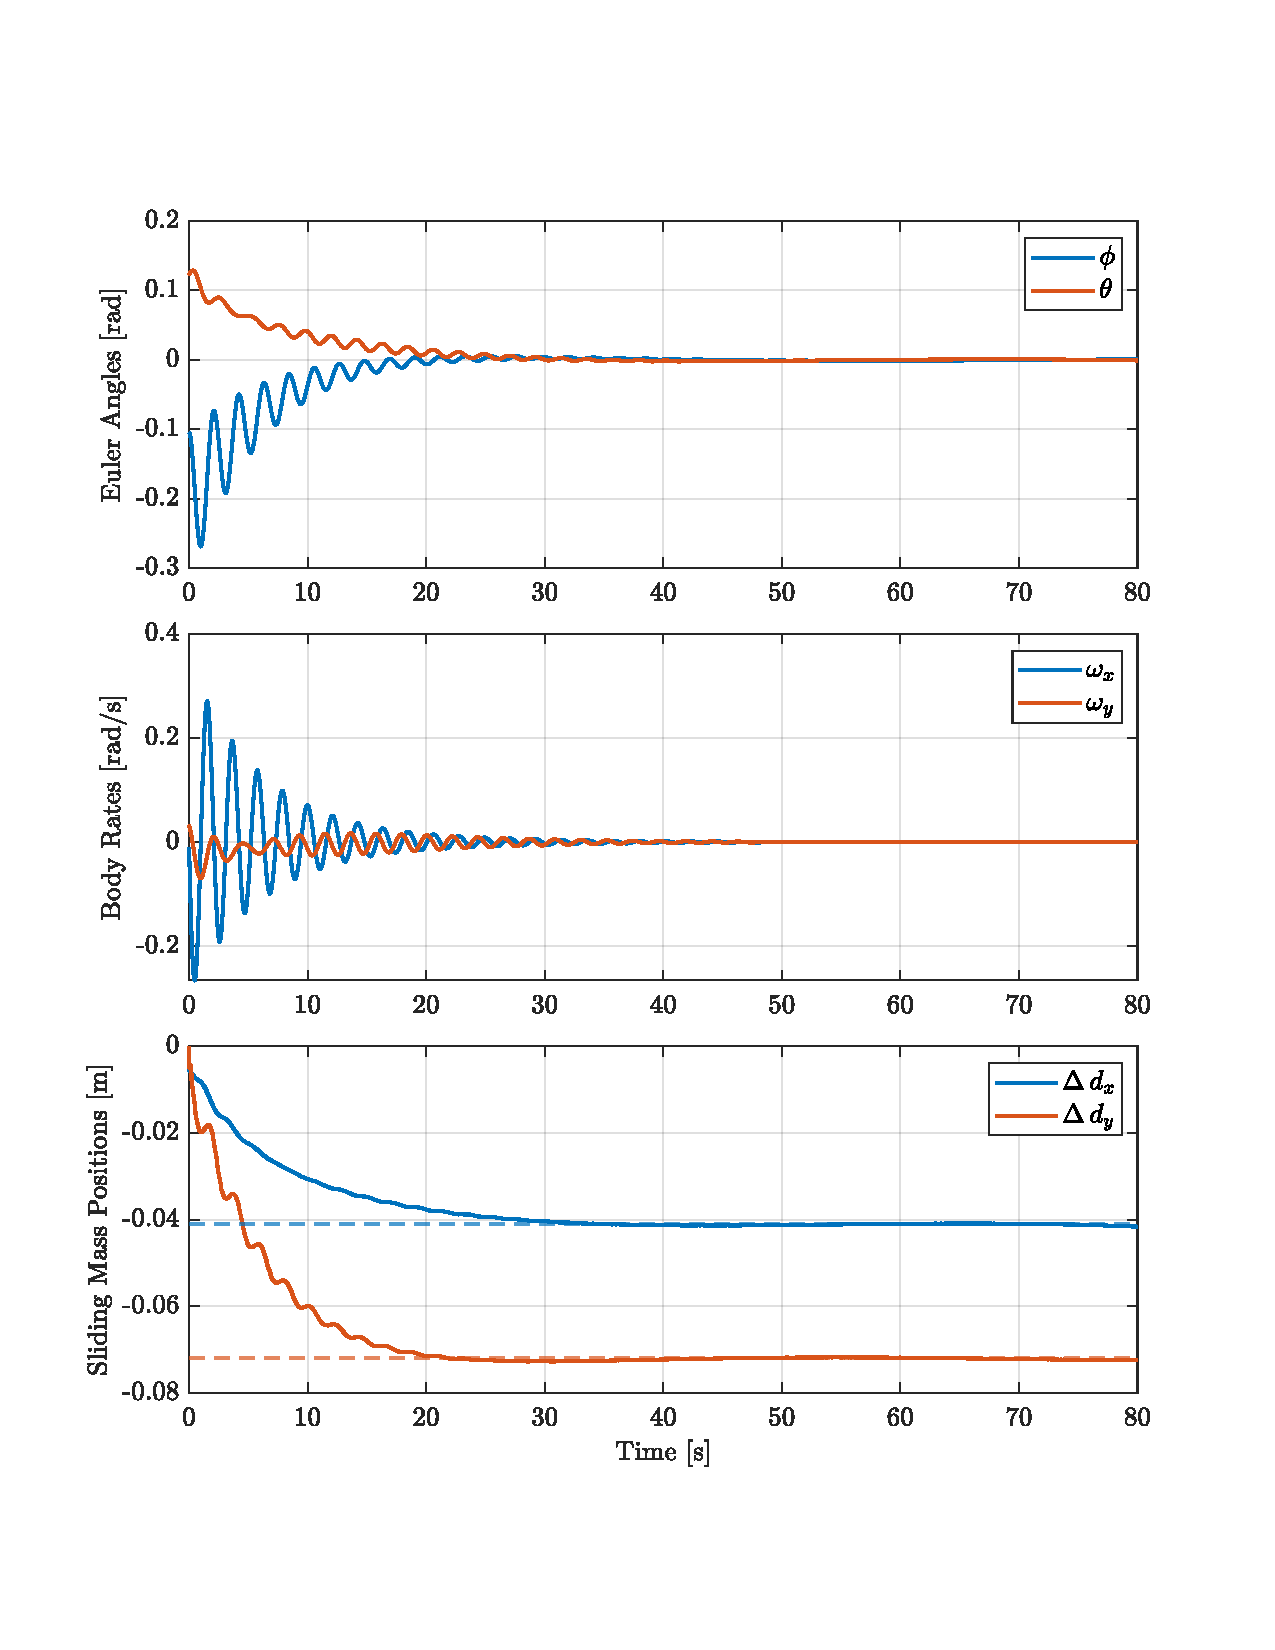
\includegraphics[width=\linewidth]{plots/PID_sim_results.pdf}
    \caption{Simulated balancing results using PID control}
\end{figure}

\begin{figure}[!ht]
    \centering
    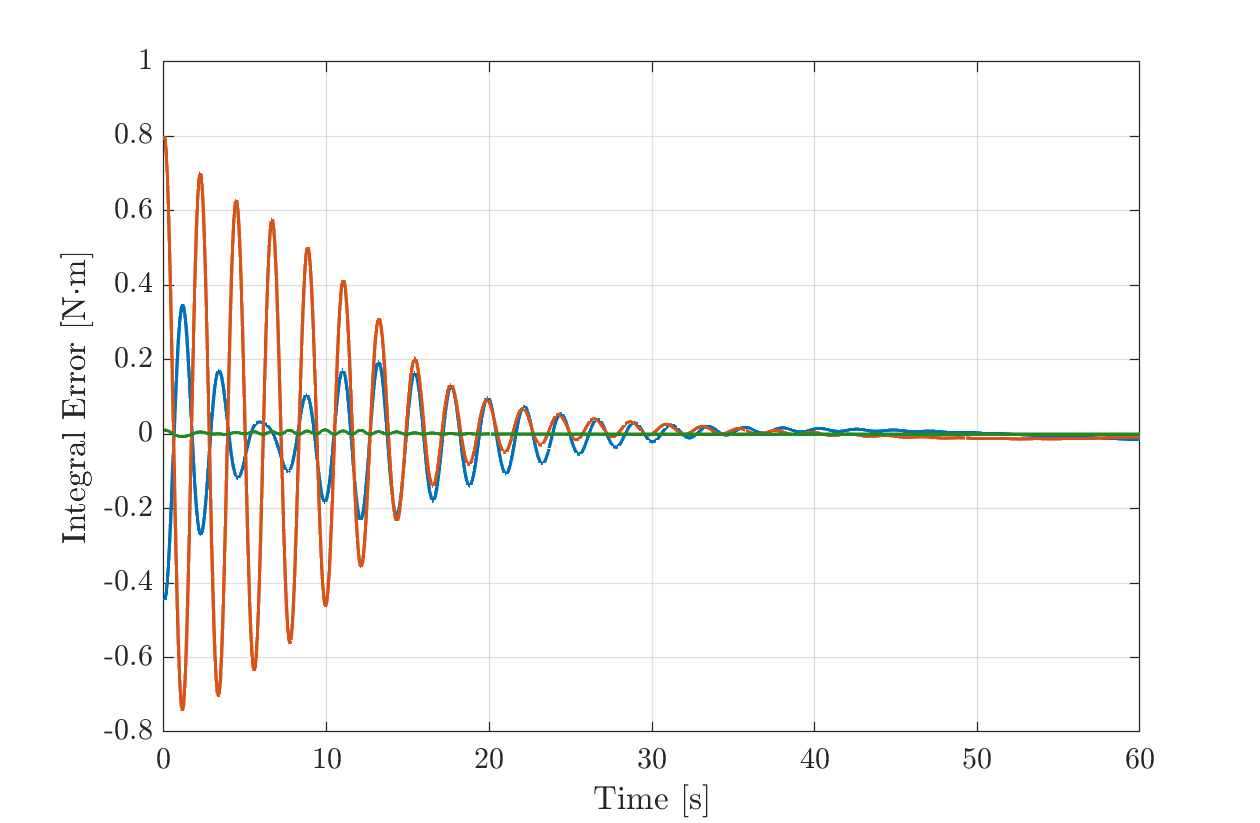
\includegraphics[width=\linewidth]{plots/PID_sim_integral_error.png}
    \caption{Projected integral error during a simulated PID run}
\end{figure}

\begin{figure}[!ht]
    \centering
    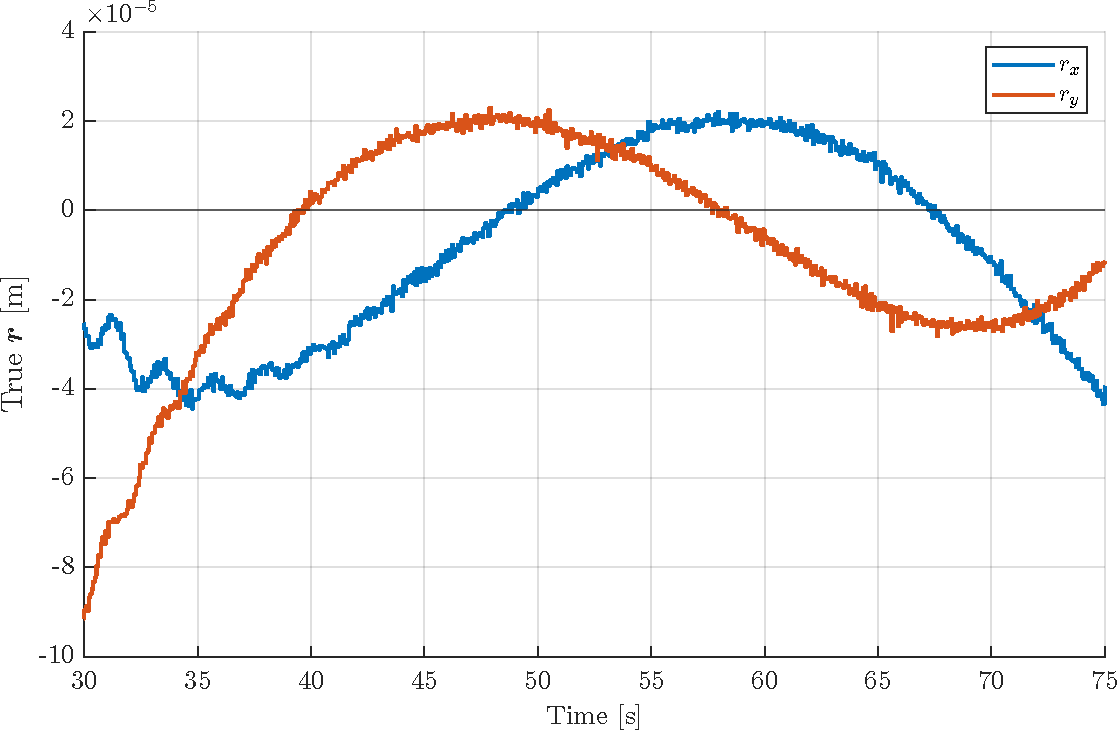
\includegraphics[width=\linewidth]{plots/PID_sim_oscillations.pdf}
    \caption{Simulated PID scillatations about $\bm{r}=0$ at steady state}
\end{figure}



\begin{figure}[!ht]
    \centering
    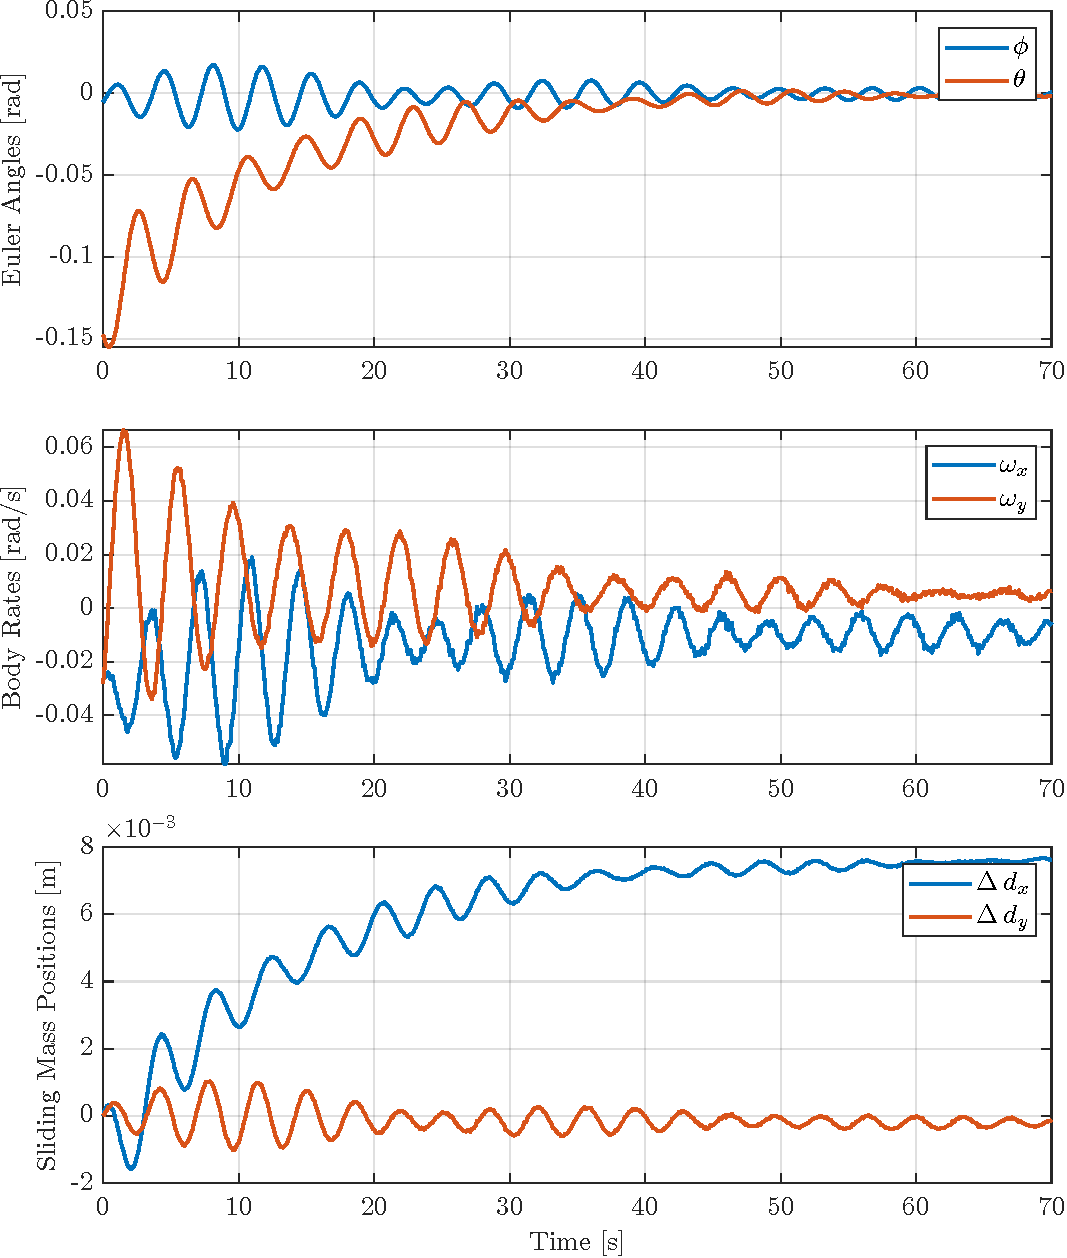
\includegraphics[width=\linewidth]{plots/PID_hardware_results.pdf}
    \caption{Experimental balancing results using PID control}
\end{figure}

\section{Underactuated Adaptive Control}

\begin{figure}[!ht]
    \centering
    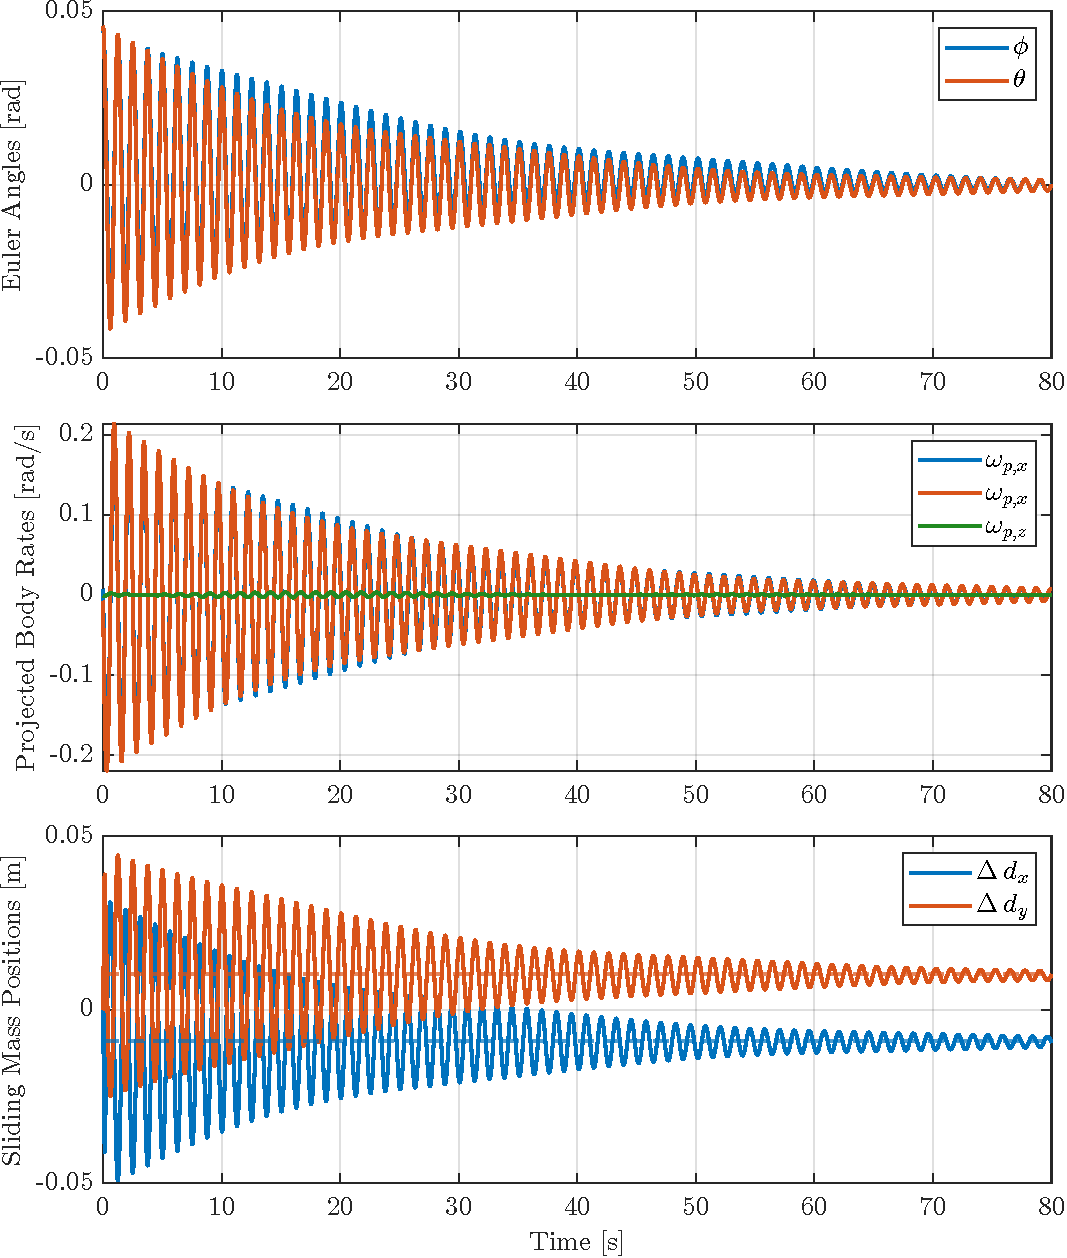
\includegraphics[width=\linewidth]{plots/adaptive_sim_success.pdf}
    \caption{Simulated underactuated adaptive control results using a simplified model}
\end{figure}

\begin{figure}[!ht]
    \centering
    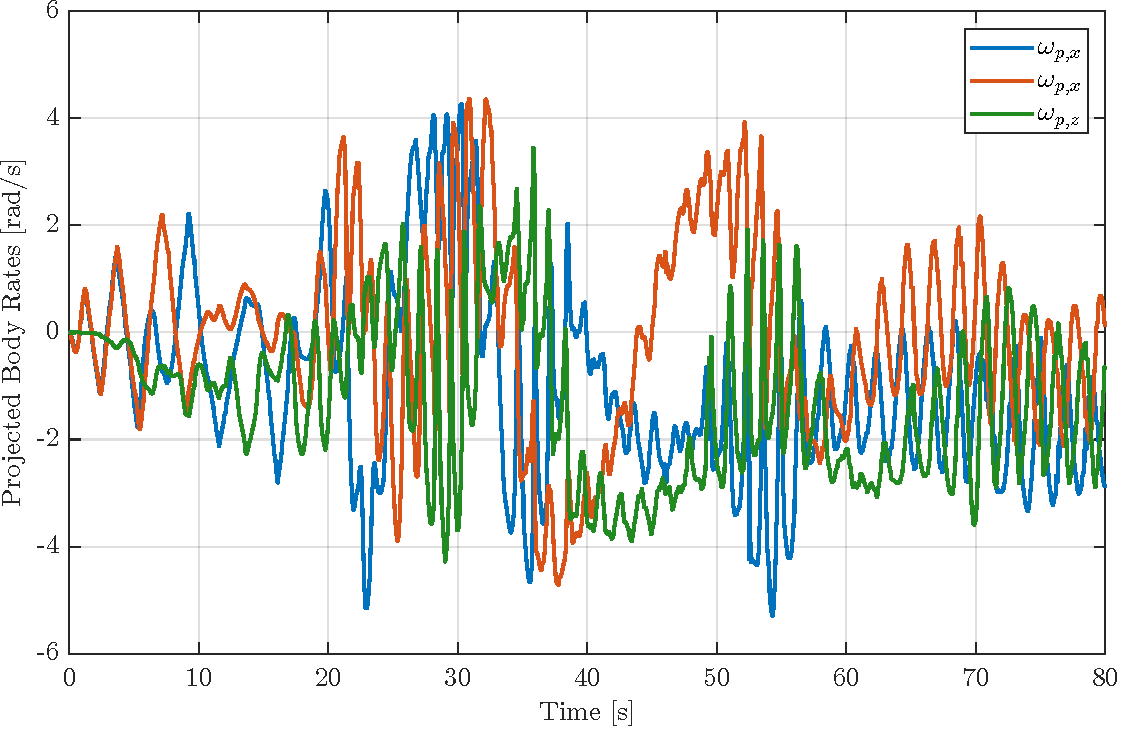
\includegraphics[width=\linewidth]{plots/adaptive_sim_failure.pdf}
    \caption{Simulated underactuated adaptive control results with sensor dyanmics and onboard filtering modeled}
\end{figure}

\begin{figure}[!ht]
    \centering
    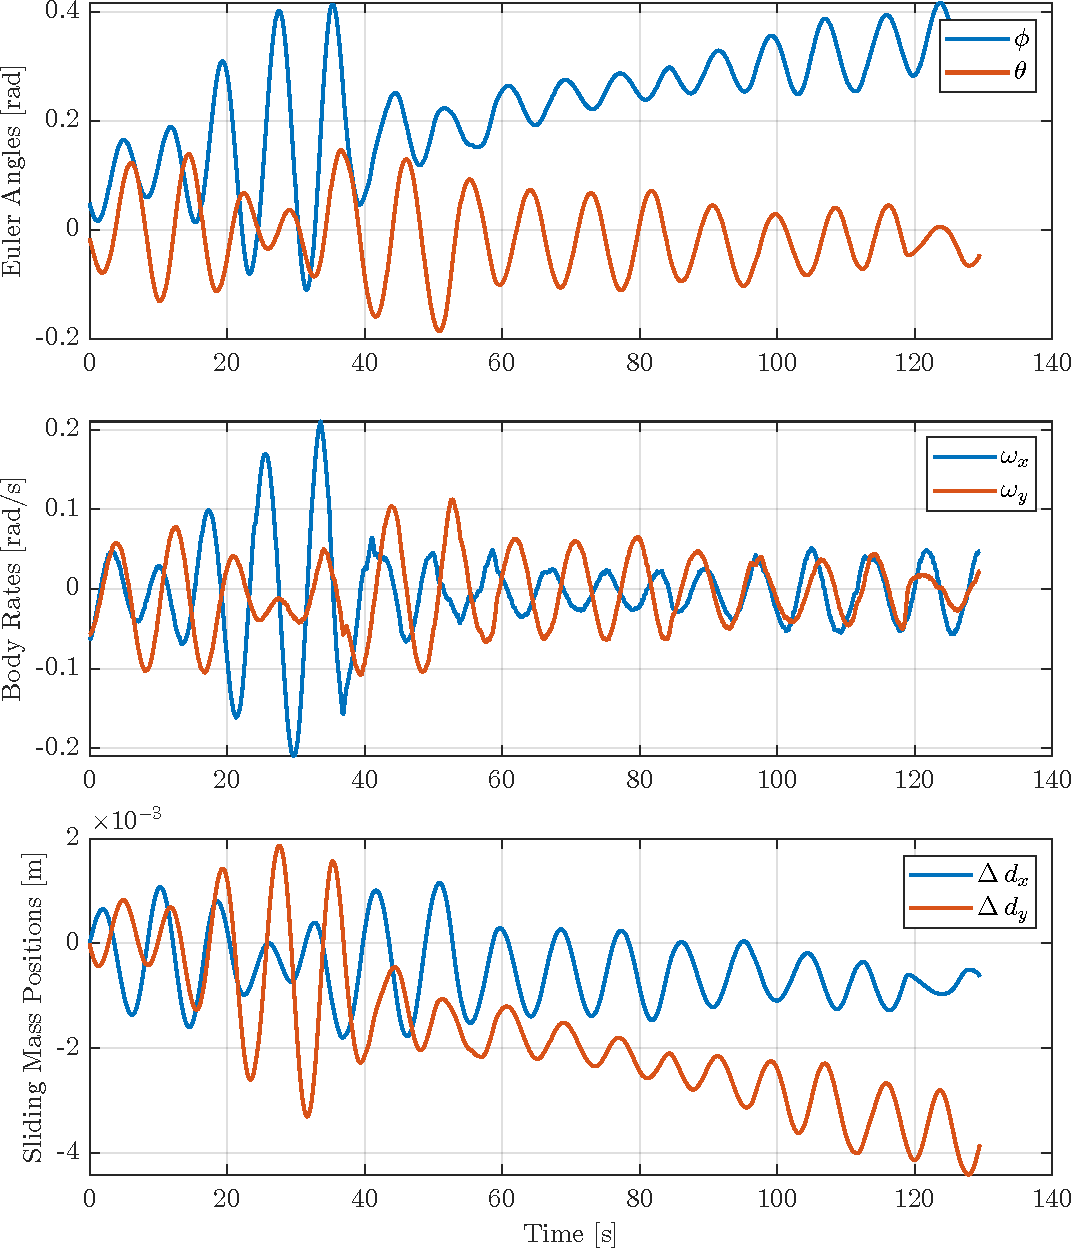
\includegraphics[width=\linewidth]{plots/adaptive_hardware_failure.pdf}
    \caption{Experimental results using underactuated adaptive control}
\end{figure}


\section{Vertical Inbalance Estimation with Kalman Filtering}

\begin{figure}[!ht]
  \centering
  \begin{subfigure}[t]{0.47\textwidth}
    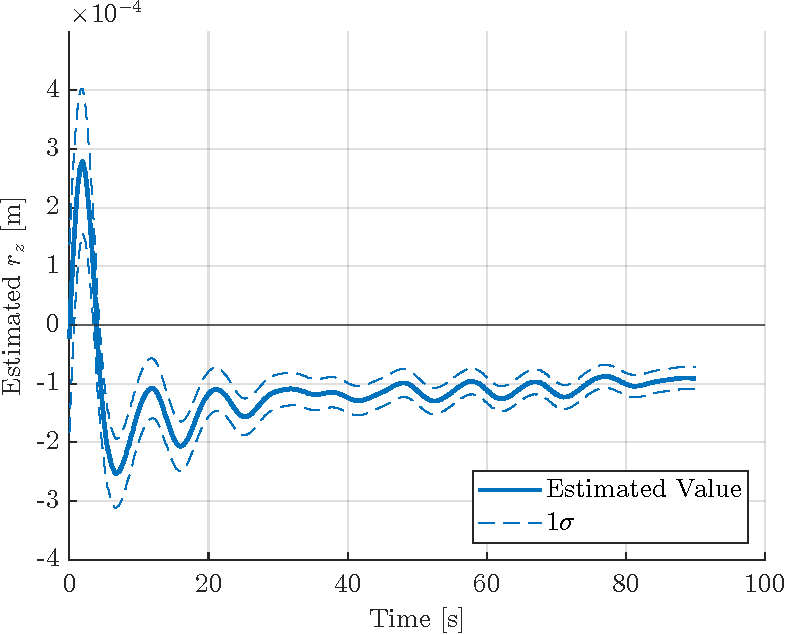
\includegraphics[width=\linewidth]{plots/UKF_hardware_success.pdf}
    \caption{Iteration successfully converging}\label{fig:a}
  \end{subfigure}\hfill
  \begin{subfigure}[t]{0.47\textwidth}
    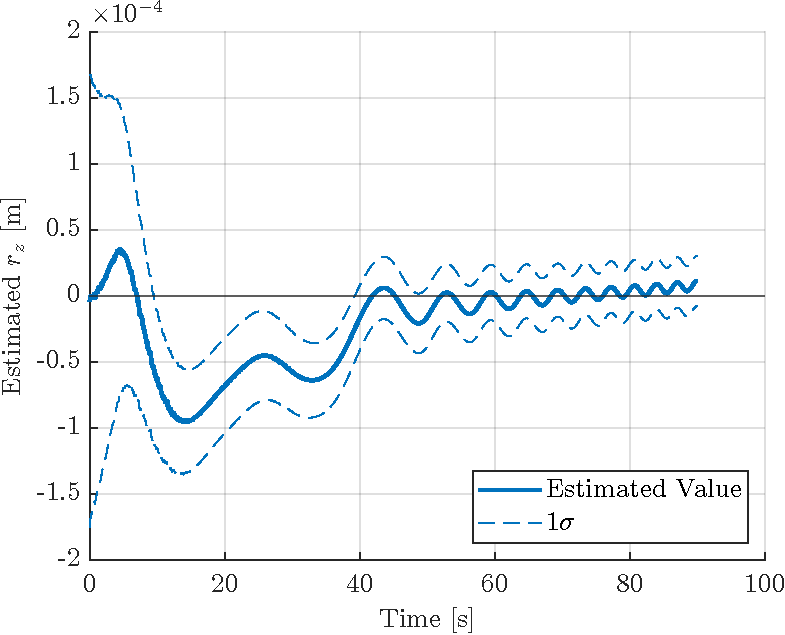
\includegraphics[width=\linewidth]{plots/UKF_hardware_failure.pdf}
    \caption{Iteration failing to converge}\label{fig:b}
  \end{subfigure}
  \caption{Experimental filter output during vertical inbalance estimation}
  \label{fig:twopanels}
\end{figure}

\begin{figure}[!ht]
  \centering
  \begin{subfigure}[t]{0.47\textwidth}
    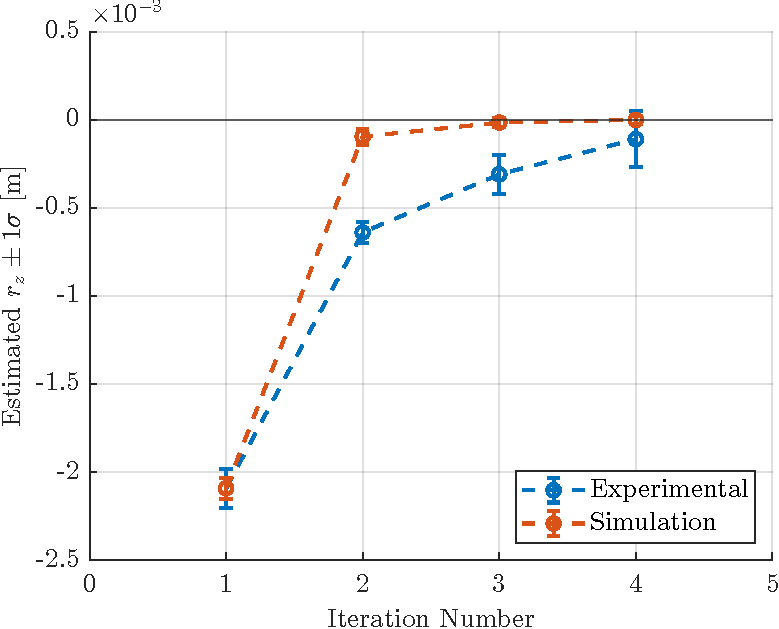
\includegraphics[width=\linewidth]{plots/UKF_comparison.pdf}
    \label{fig:a}
  \end{subfigure}\hfill
  \begin{subfigure}[t]{0.47\textwidth}
    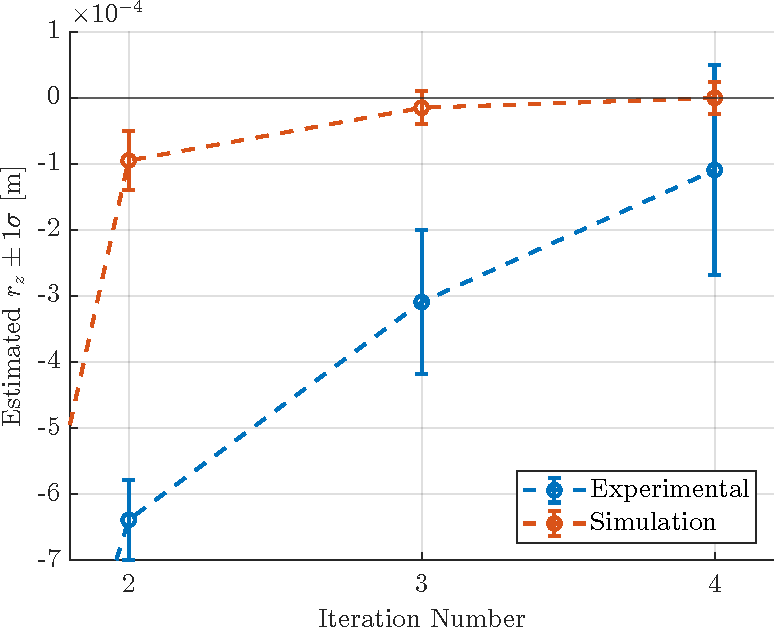
\includegraphics[width=\linewidth]{plots/UKF_comparison_zoomed.pdf}

    \label{fig:b}
  \end{subfigure}
  \caption{Filter results over multiple iterations, zoomed in on right}
  \label{fig:twopanels}
\end{figure}



\section{Passive Balancing Using Least-Squares Estimation}
% experimental results only use 1 RW
% simulation results should include 1 RW and 4 RWs to compare (unless the one RW setup turns out good)

\begin{figure}[!ht]
  \centering
  \begin{subfigure}[t]{0.47\textwidth}
    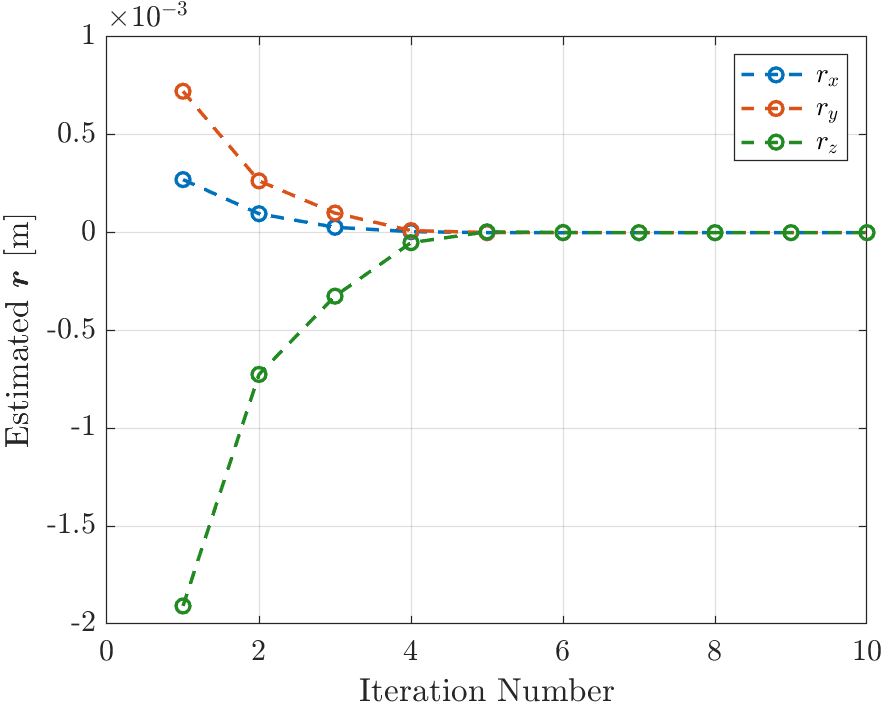
\includegraphics[width=\linewidth]{plots/LSR_sim_all_runs.png}
    \caption{All 10 iterations}\label{fig:a}
  \end{subfigure}\hfill
  \begin{subfigure}[t]{0.47\textwidth}
    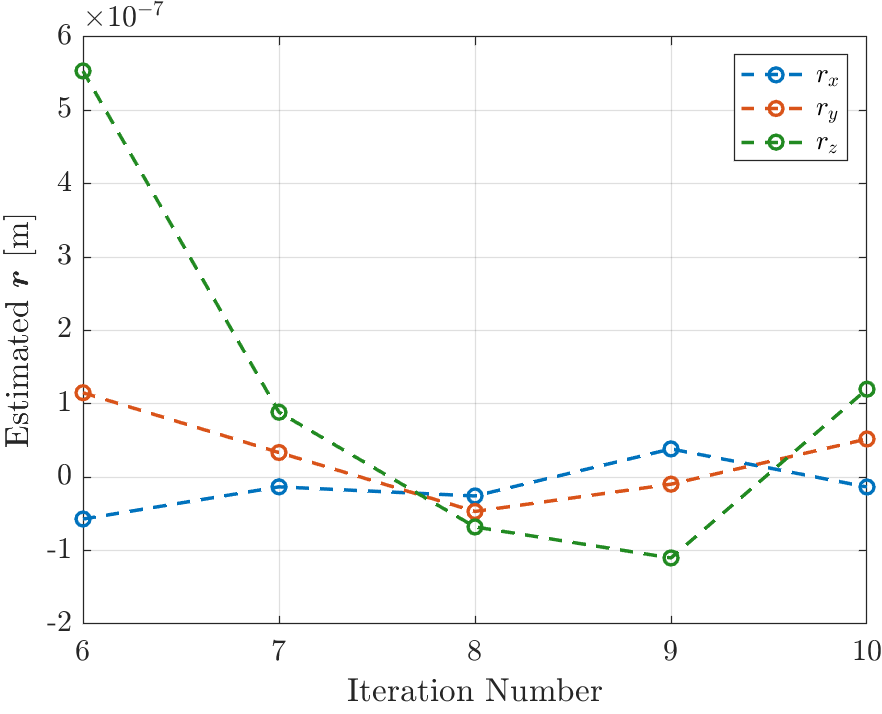
\includegraphics[width=\linewidth]{plots/LSR_sim_last_5_runs.png}
    \caption{Final 5 iterations}\label{fig:b}
  \end{subfigure}
  \caption{Simulated results of least-squares estimation method}
  \label{fig:twopanels}
\end{figure}

\begin{figure}[!ht]
    \centering
    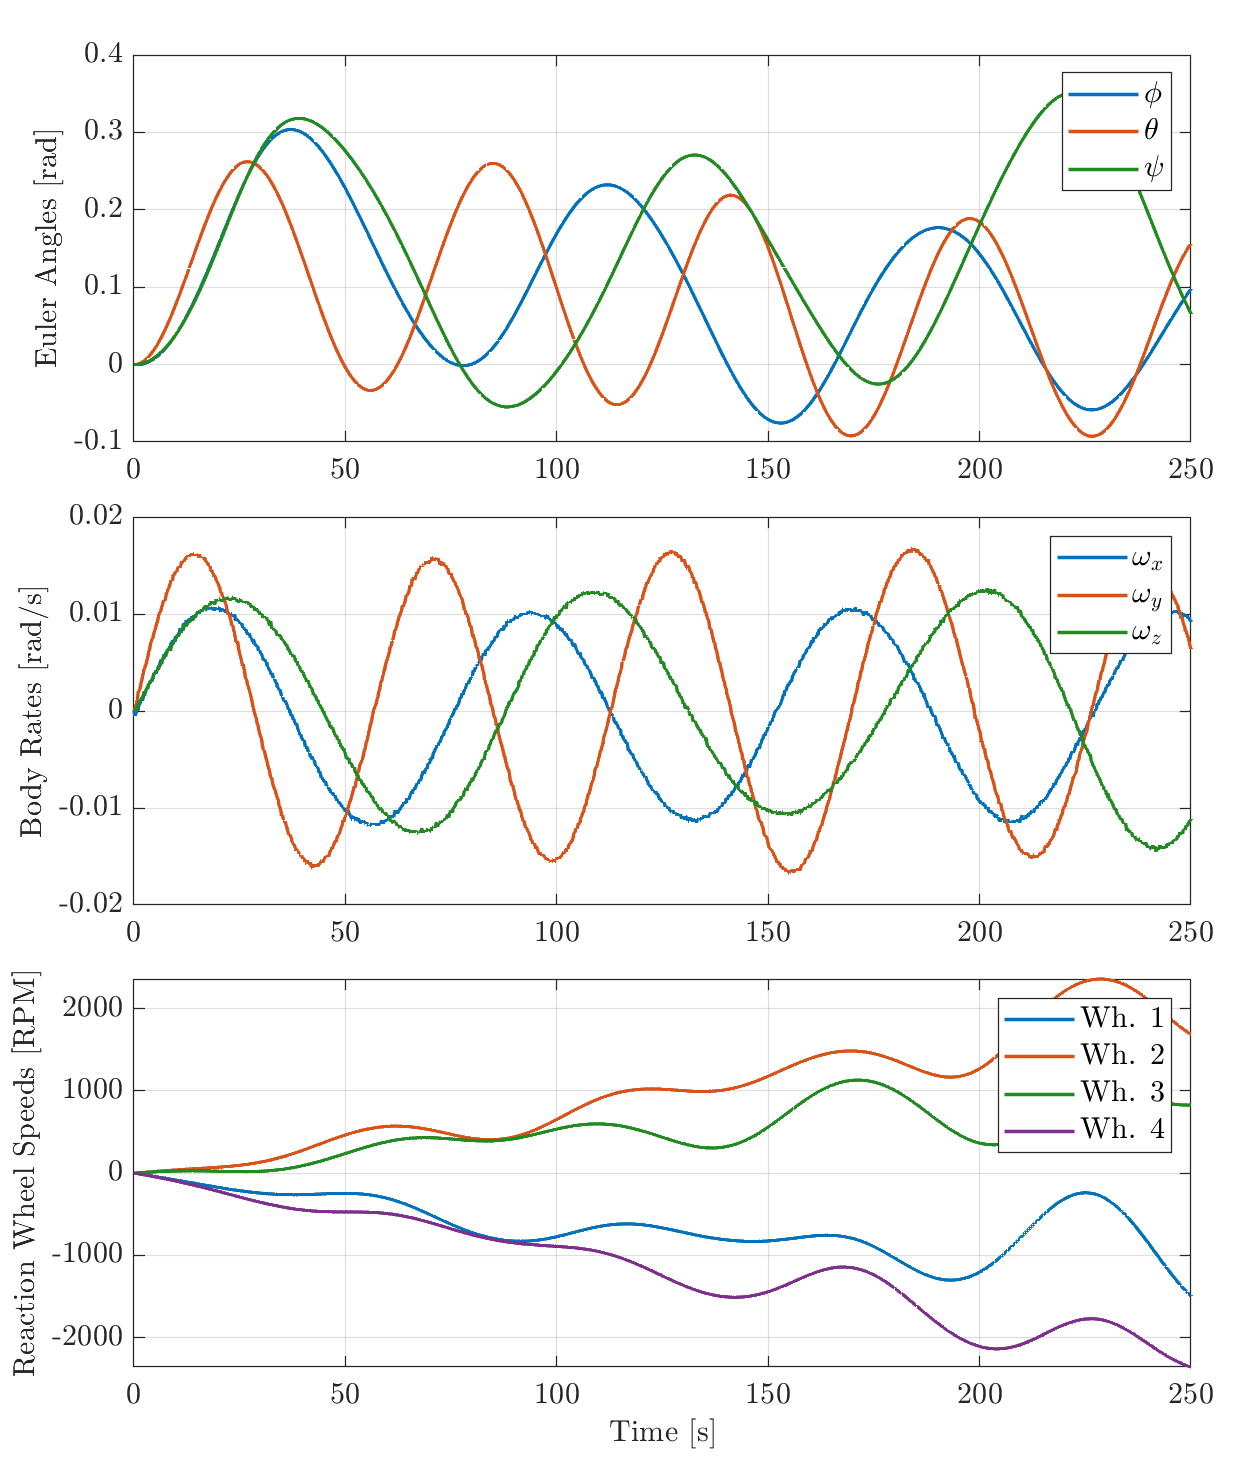
\includegraphics[width=\linewidth]{plots/LSR_sim_excitation}
    \caption{Simulated platform excitation during batch estimation}
\end{figure}

\begin{figure}[!ht]
    \centering
    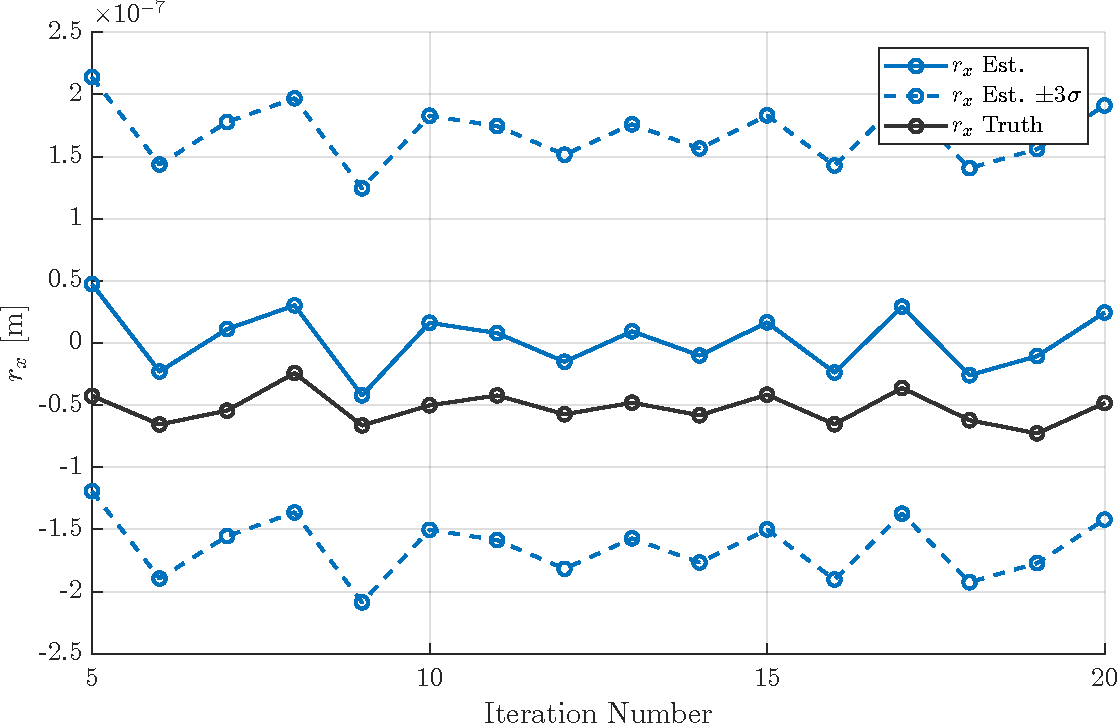
\includegraphics[width=\linewidth]{plots/LSR_sim_confidence.pdf}
    \caption{Comparison between estimated and true values}
\end{figure}

\begin{figure}[!ht]
  \centering
  \begin{subfigure}[t]{0.47\textwidth}
    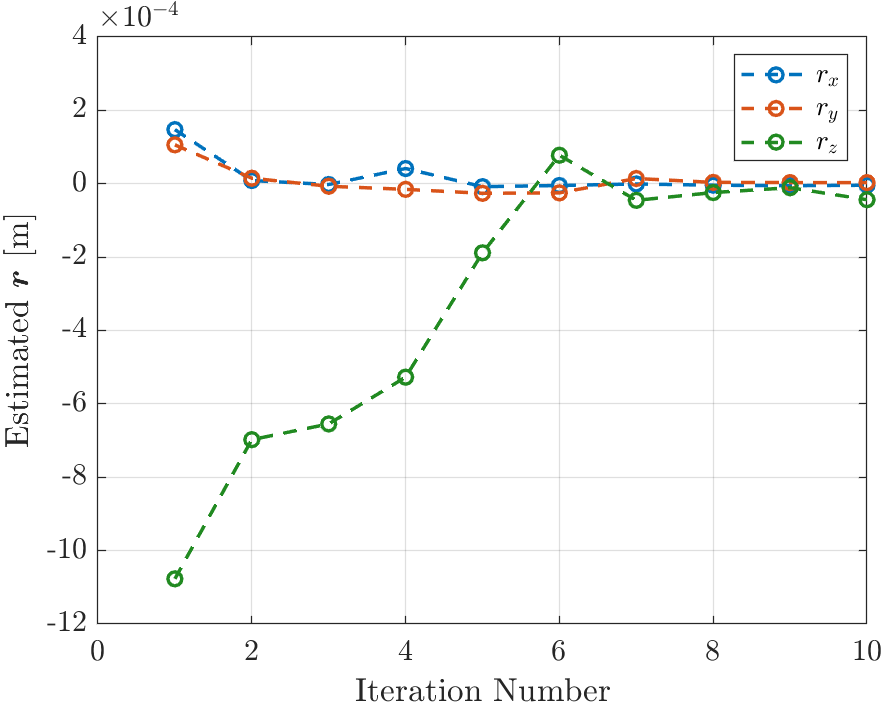
\includegraphics[width=\linewidth]{plots/LSR_hardware_all_runs.png}
    \caption{All 10 iterations}\label{fig:a}
  \end{subfigure}\hfill
  \begin{subfigure}[t]{0.47\textwidth}
    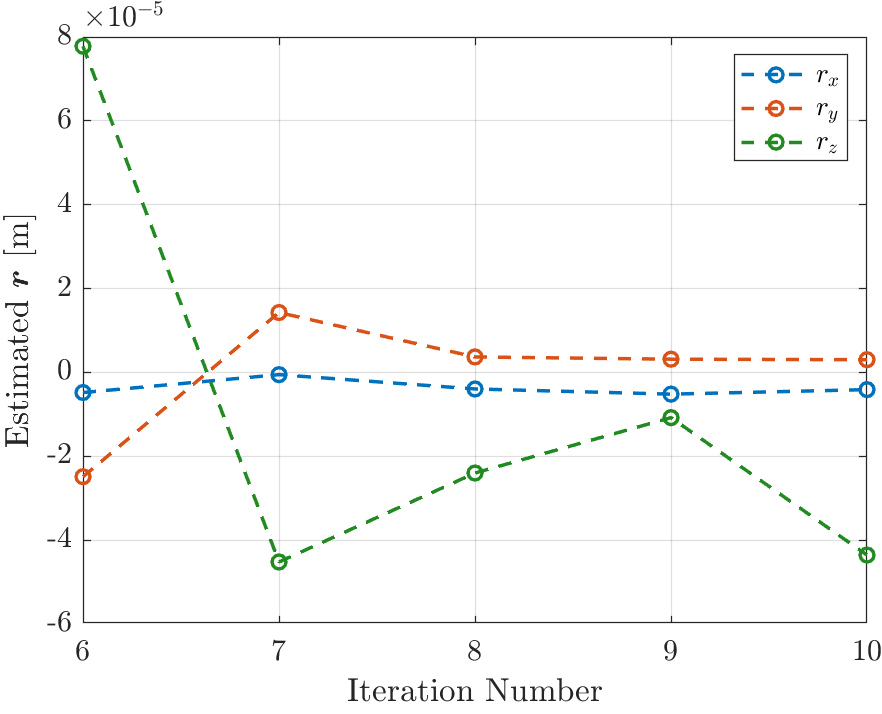
\includegraphics[width=\linewidth]{plots/LSR_hardware_last_5_runs.png}
    \caption{Final 5 iterations}\label{fig:b}
  \end{subfigure}
  \caption{Experimental results of least-squares estimation method}
  \label{fig:LSR_hardware_iterations}
\end{figure}

\begin{figure}[!ht]
    \centering
    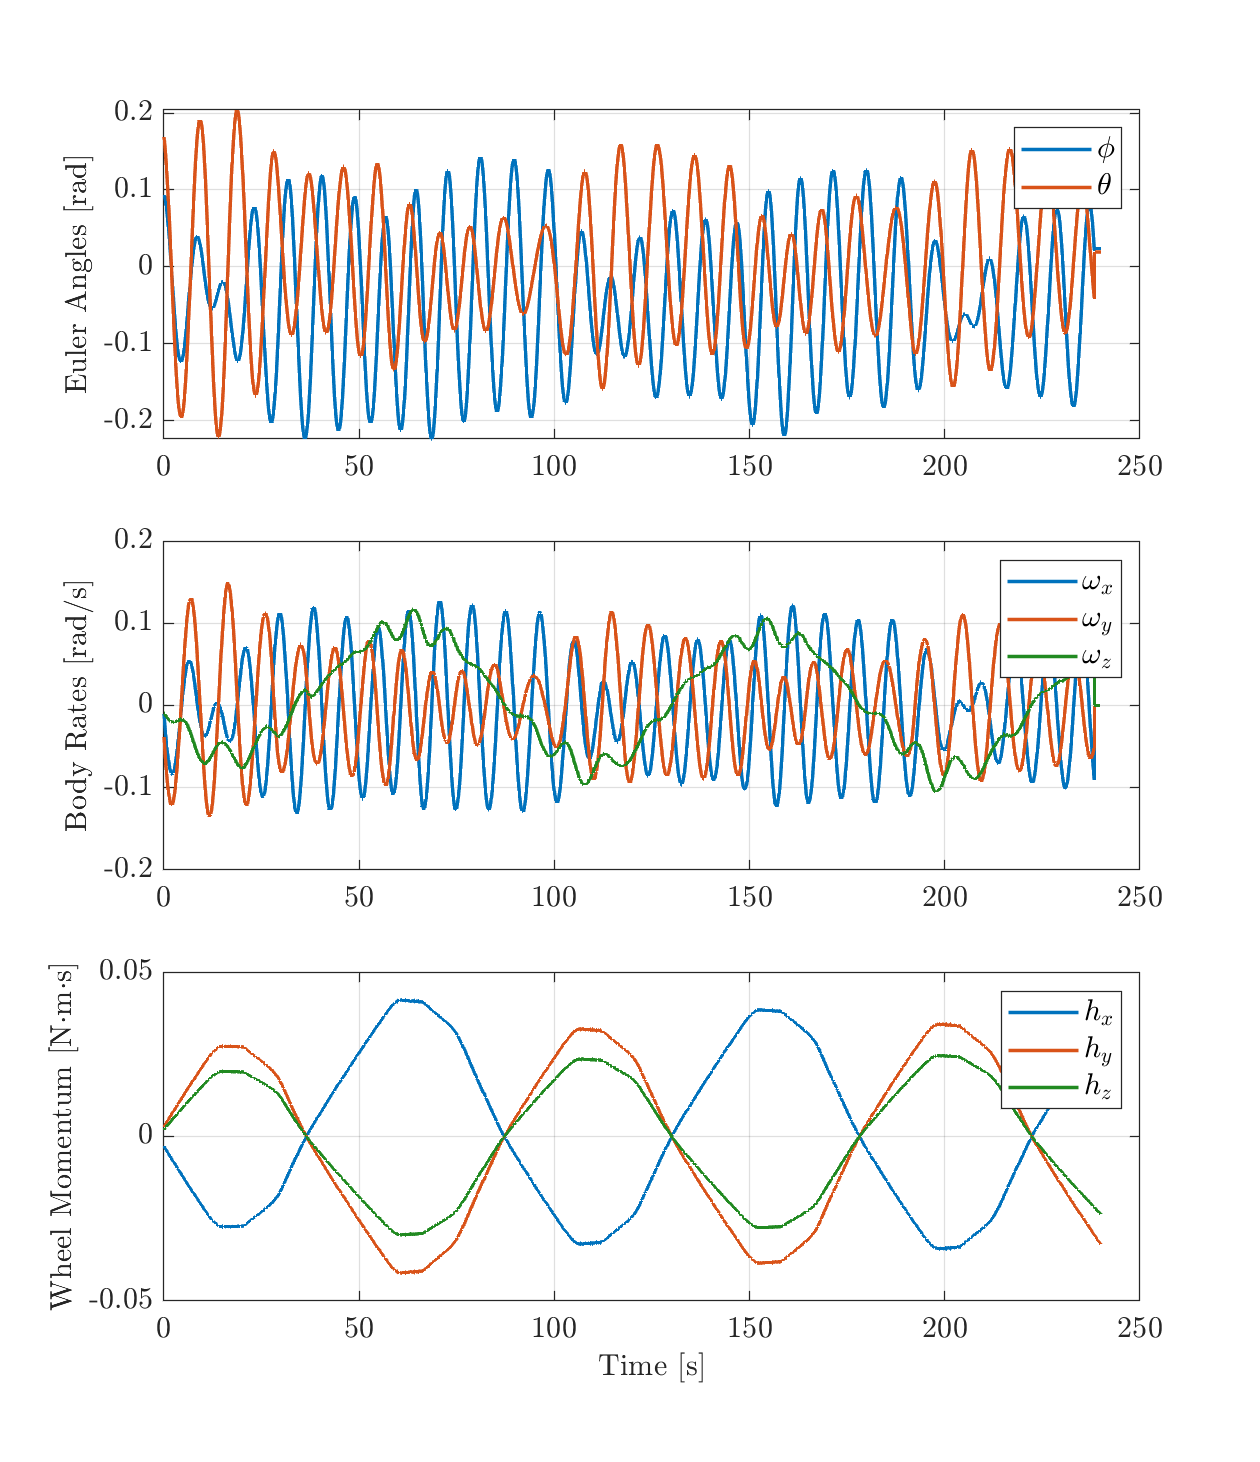
\includegraphics[width=\linewidth]{plots/LSR_hardware_excitation}
    \caption{Experimental platform excitation during batch estimation}
\end{figure}

\section{Active Balancing Using Adaptive Control}

\subsection{No Reaction Wheels}
% the experimental results for this are in a seperate repo - SADS Adaptive

\subsection{Full Reaction Wheel Setup - Simulink Only}

\begin{figure}[!ht]
    \centering
    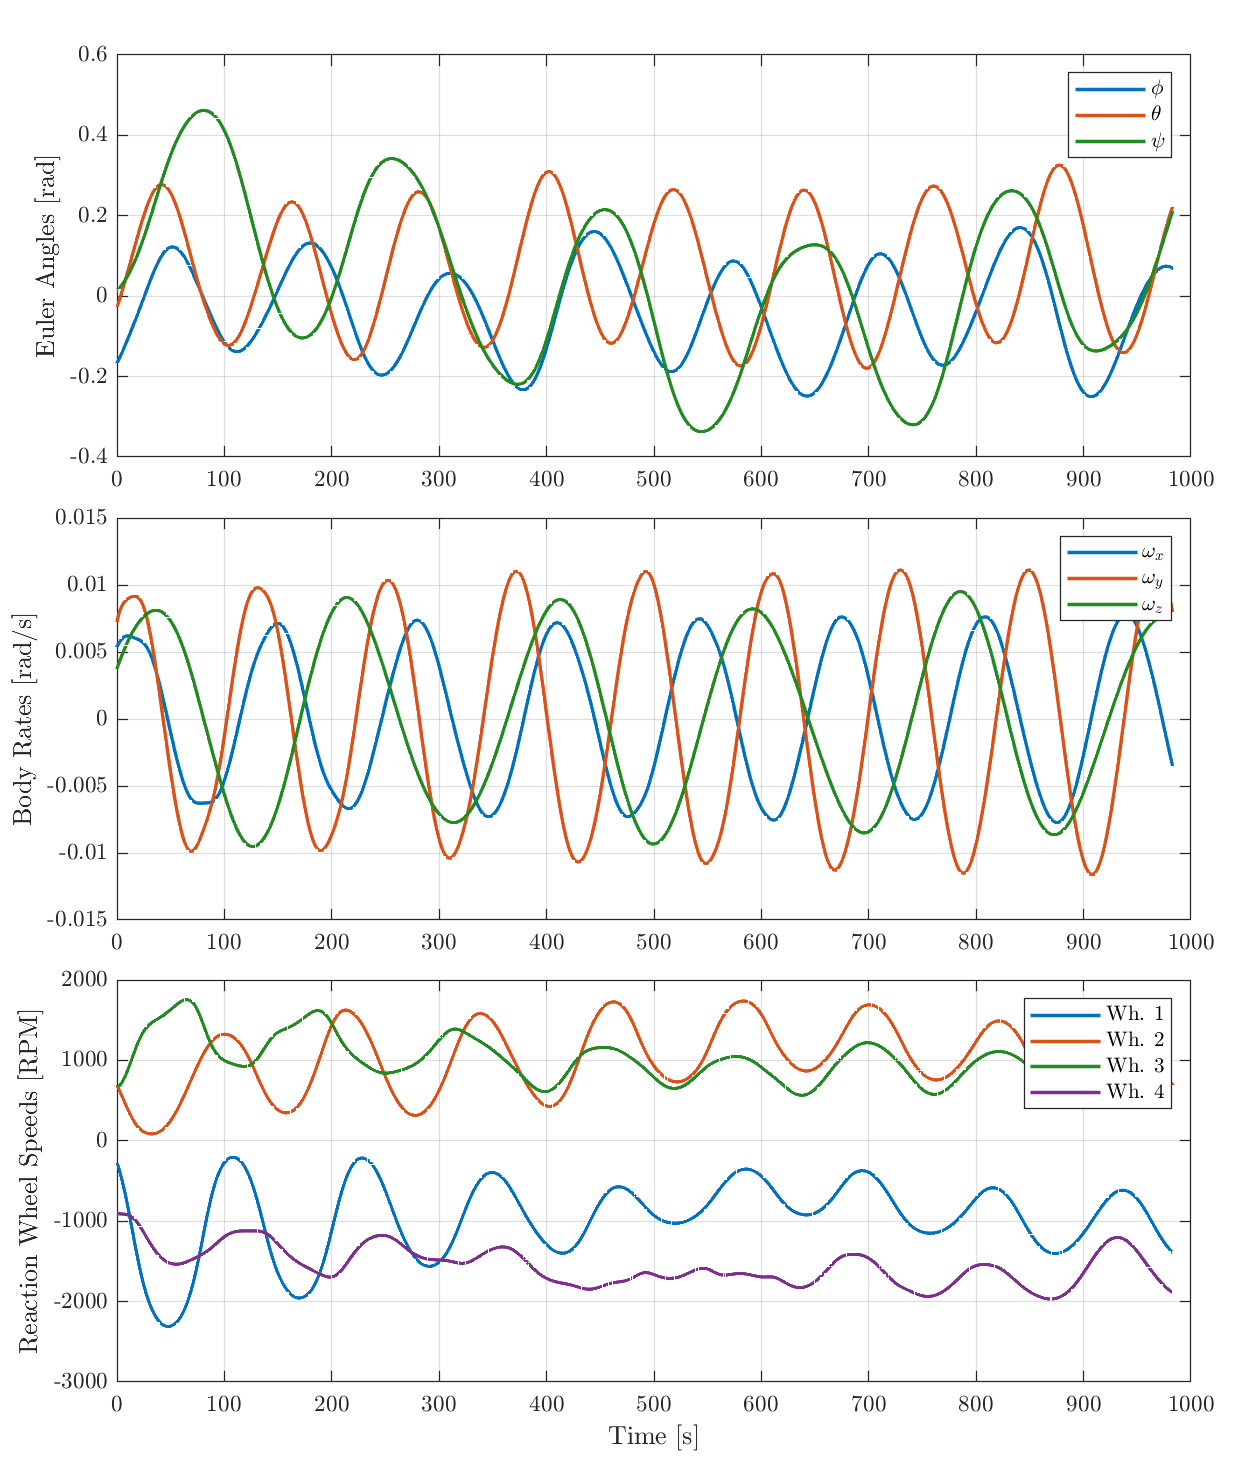
\includegraphics[width=\linewidth]{plots/three_axis_sim_excitation.png}
    \caption{Simulated platform excitation for 3-axis adaptive control}
\end{figure}

\begin{figure}[!ht]
  \centering
  \begin{subfigure}[t]{0.47\textwidth}
    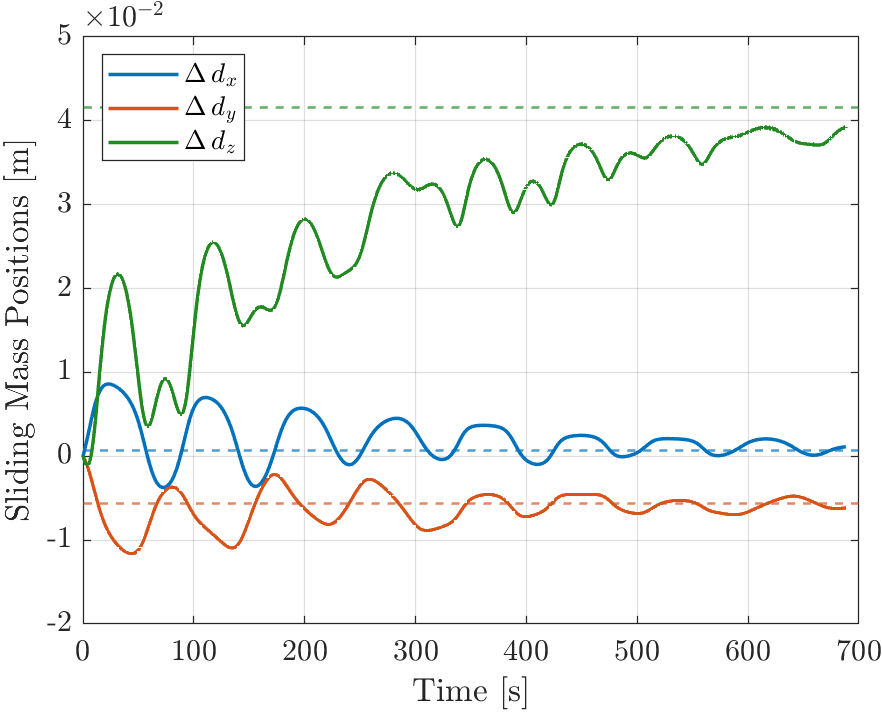
\includegraphics[width=\linewidth]{plots/three_axis_sim_positions_1.png}
    \caption{1st iteration}\label{fig:a}
  \end{subfigure}\hfill
  \begin{subfigure}[t]{0.47\textwidth}
    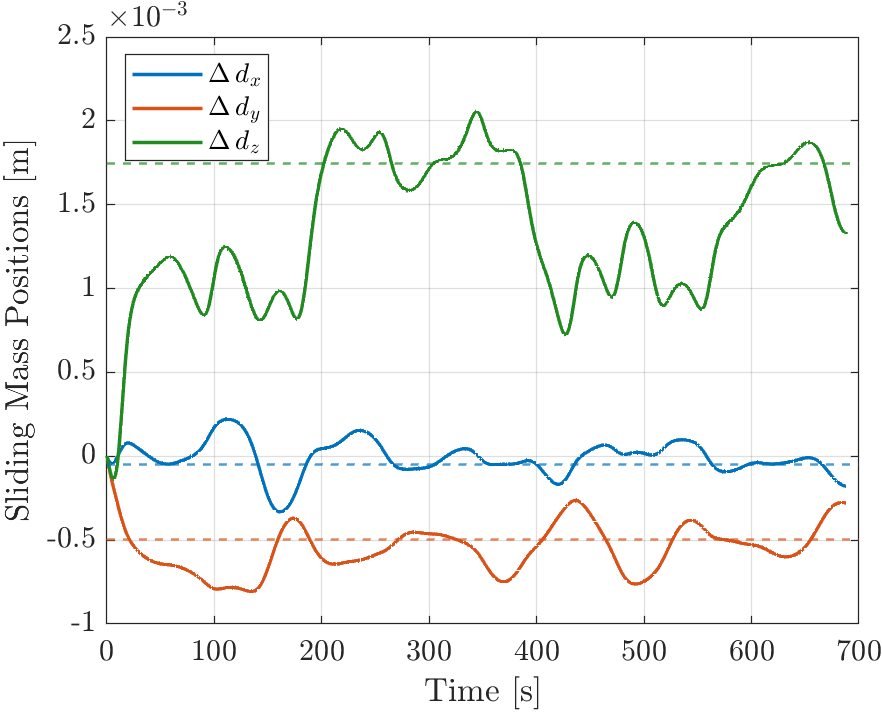
\includegraphics[width=\linewidth]{plots/three_axis_sim_positions_2.png}
    \caption{2nd iteration}\label{fig:b}
  \end{subfigure}
  \caption{Simulated sliding mass positions during 3-axis adaptive control}
  \label{fig:LSR_hardware_iterations}
\end{figure}

\begin{figure}[!ht]
    \centering
    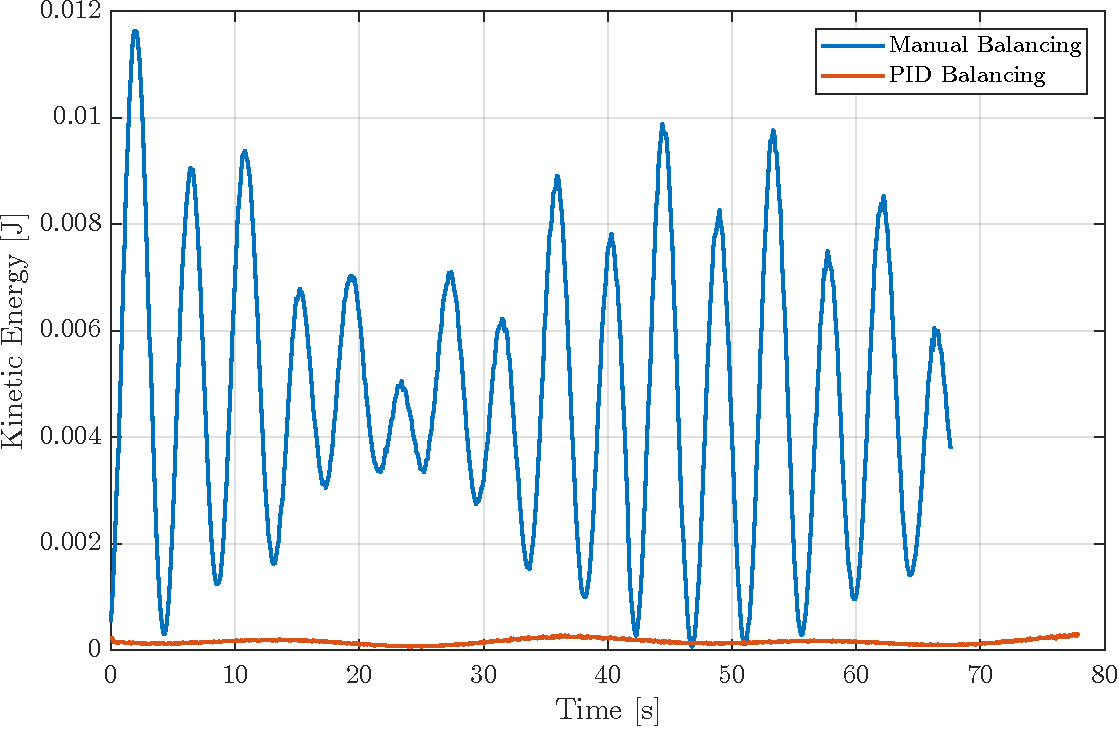
\includegraphics[width=\linewidth]{plots/hardware_verification_KE.pdf}
    \caption{Kinetic energy of the simulator before and after using two-step PID balancing}
\end{figure}



\iffalse
SIM RESULTS ------------------------------
Results PID:
horizontal: 2.5e-5
verit 6.7e-7
KE = 0.0134
torque = 0.010146

Results Batch:
horizontal: 1e-7
vert: 2.2e-7

Results UKF
r_z = 6.784e-07

Results 3-axis
horizontal: 4.8261e-06
vertical: 9.7241e-05
KE = 0.042205
torque = 0.01883
\fi

\chapter{Conclusion} \label{chap:conclusion}

    %% Bibliography/references section
    %% Difference between Biblography and References
%
% A bibliography is a collection of resources that you found of value
% related to your thesis. It includes all items that you cited in your
% thesis as well as any other valuable references.
%
% On the other hand, a references section is just the items that you cited
% in your thesis.

% For a bibliography, put all references you want in your bibliography
% into your bib-file, then use the following line:
\nocite{*}

% For a references section use the following line:
%\renewcommand{\bibname}{References}

    \printbibliography[
        heading=bibintoc,
        title={\MakeUppercase{\bibname}}
    ]

    %% Input the appendices (if any) as configured from the file
    % % If have only one appendix pass the number of appendices, 1,
% to the appendix command as an optional parameter:
%\appendix[1]
% If have multiple appendices can pass the number of appendices
% to the appendix command as an optional parameter or omit it:
\appendix

\chapter{First Appendix}
    \lipsum[1]
    \begin{table}
        \centering
        \begin{tabular}{r r r r r r r r}
             Col1 & Col2 & Col3 & Col4 & Col1 & Col2 & Col3 & Col4 \\
             \hline
             1    & 676  & 8837 & 787  & 544  & 22   & 908  & 229  \\
             2    & 732  & 78   & 5415 & 887  & 343  & 1112 & 870  \\
             3    & 545  & 778  & 7507 & 5554 & 5432 & 9867 & 9    \\
             4    & 545  & 1874 & 7560 & 102  & 562  & 223  & 792  \\
             5    & 88   & 788  & 6344 & 45   & 998  & 776  & 2    \\
             \hline
        \end{tabular}
        \caption{This is the caption for the first table.}
    \end{table}
    \lipsum[2]

\section{A Section}
    \lipsum[3]
    \begin{table}
        \centering
        \begin{tabular}{r r r r r r r r}
             Col1 & Col2 & Col3 & Col4 & Col1 & Col2 & Col3 & Col4 \\
             \hline
             1    & 676  & 8837 & 787  & 544  & 22   & 908  & 229  \\
             2    & 732  & 78   & 5415 & 887  & 343  & 1112 & 870  \\
             3    & 545  & 778  & 7507 & 5554 & 5432 & 9867 & 9    \\
             4    & 545  & 1874 & 7560 & 102  & 562  & 223  & 792  \\
             5    & 88   & 788  & 6344 & 45   & 998  & 776  & 2    \\
             \hline
        \end{tabular}
        \caption{This is the caption for another table.}
    \end{table}
    \lipsum[4-5]
    \begin{figure}
        \centering
        \includegraphics[width=3.5in]{example-image}
        \caption{This is the caption for first image.}
    \end{figure}

\subsection{A Subsection}
    \lipsum[6-8]
    \begin{figure}
        \centering
        \includegraphics{example-image-golden}
        \caption{This is the caption for another image where the description is rather long and will probably go beyond one line.}
    \end{figure}

\section{Another Section}
    \lipsum[1-2]
    \begin{table}
        \centering
        \begin{tabular}{r r r r r r r r}
             Col1 & Col2 & Col3 & Col4 & Col1 & Col2 & Col3 & Col4 \\
             \hline
             1    & 676  & 8837 & 787  & 544  & 22   & 908  & 229  \\
             2    & 732  & 78   & 5415 & 887  & 343  & 1112 & 870  \\
             3    & 545  & 778  & 7507 & 5554 & 5432 & 9867 & 9    \\
             4    & 545  & 1874 & 7560 & 102  & 562  & 223  & 792  \\
             5    & 88   & 788  & 6344 & 45   & 998  & 776  & 2    \\
             \hline
        \end{tabular}
        \caption{This is the caption for yet another table.}
    \end{table}

\subsection{Another Subsection}
    \lipsum[3-5]

\subsubsection{A Sub-Subsection}
    \lipsum[6-8]


\chapter{Second Appendix}
    \lipsum[1]
    \begin{table}
        \centering
        \begin{tabular}{r r r r r r r r}
             Col1 & Col2 & Col3 & Col4 & Col1 & Col2 & Col3 & Col4 \\
             \hline
             1    & 676  & 8837 & 787  & 544  & 22   & 908  & 229  \\
             2    & 732  & 78   & 5415 & 887  & 343  & 1112 & 870  \\
             3    & 545  & 778  & 7507 & 5554 & 5432 & 9867 & 9    \\
             4    & 545  & 1874 & 7560 & 102  & 562  & 223  & 792  \\
             5    & 88   & 788  & 6344 & 45   & 998  & 776  & 2    \\
             \hline
        \end{tabular}
        \caption{This is the caption for the first table.}
    \end{table}
    \lipsum[2]

\section{A Section}
    \lipsum[3]
    \begin{table}
        \centering
        \begin{tabular}{r r r r r r r r}
             Col1 & Col2 & Col3 & Col4 & Col1 & Col2 & Col3 & Col4 \\
             \hline
             1    & 676  & 8837 & 787  & 544  & 22   & 908  & 229  \\
             2    & 732  & 78   & 5415 & 887  & 343  & 1112 & 870  \\
             3    & 545  & 778  & 7507 & 5554 & 5432 & 9867 & 9    \\
             4    & 545  & 1874 & 7560 & 102  & 562  & 223  & 792  \\
             5    & 88   & 788  & 6344 & 45   & 998  & 776  & 2    \\
             \hline
        \end{tabular}
        \caption{This is the caption for another table.}
    \end{table}
    \lipsum[4-5]
    \begin{figure}
        \centering
        \includegraphics[width=3.5in]{example-image}
        \caption{This is the caption for first image.}
    \end{figure}

\subsection{A Subsection}
    \lipsum[6-8]
    \begin{figure}
        \centering
        \includegraphics{example-image-golden}
        \caption{This is the caption for another image where the description is rather long and will probably go beyond one line.}
    \end{figure}

\section{Another Section}
    \lipsum[1-2]
    \begin{table}
        \centering
        \begin{tabular}{r r r r r r r r}
             Col1 & Col2 & Col3 & Col4 & Col1 & Col2 & Col3 & Col4 \\
             \hline
             1    & 676  & 8837 & 787  & 544  & 22   & 908  & 229  \\
             2    & 732  & 78   & 5415 & 887  & 343  & 1112 & 870  \\
             3    & 545  & 778  & 7507 & 5554 & 5432 & 9867 & 9    \\
             4    & 545  & 1874 & 7560 & 102  & 562  & 223  & 792  \\
             5    & 88   & 788  & 6344 & 45   & 998  & 776  & 2    \\
             \hline
        \end{tabular}
        \caption{This is the caption for yet another table.}
    \end{table}

\subsection{Another Subsection}
    \lipsum[3-5]
    \begin{figure}
        \centering
        \includegraphics[width=3.5in]{example-image-a}
        \caption{This is the caption for an image.}
    \end{figure}

\subsubsection{A Sub-Subsection}
    \lipsum[6-8]


\chapter{Code Examples} \label{sec:CodeExamples}
    The following code listings are to demonstrate how code could be included in an appendix.

    \lstinputlisting[caption=fibonacci.py, label=lst:fibonaccipy]{appendices/fibonacci.py}

    \begin{lstlisting}[caption=incmatrix.py, label=lst:incmatrixpy]
import numpy as np

def incmatrix(genl1,genl2):
    m = len(genl1)
    n = len(genl2)
    M = None #to become the incidence matrix
    VT = np.zeros((n*m,1), int)  #dummy variable

    #compute the bitwise xor matrix
    M1 = bitxormatrix(genl1)
    M2 = np.triu(bitxormatrix(genl2),1)

    for i in range(m-1):
        for j in range(i+1, m):
            [r,c] = np.where(M2 == M1[i,j])
            for k in range(len(r)):
                VT[(i)*n + r[k]] = 1;
                VT[(i)*n + c[k]] = 1;
                VT[(j)*n + r[k]] = 1;
                VT[(j)*n + c[k]] = 1;

                if M is None:
                    M = np.copy(VT)
                else:
                    M = np.concatenate((M, VT), 1)

                VT = np.zeros((n*m,1), int)

    return M
    \end{lstlisting}


\end{document}
